\documentclass[a4paper, oneside, 11pt]{book}

\usepackage[english]{babel}
\usepackage[utf8x]{inputenc}
\usepackage{amsmath}
\usepackage{graphicx}
\usepackage{titlesec} 
\usepackage{color}
\usepackage{mathptmx}
\usepackage{hyperref}
\usepackage{listings}
\usepackage{eurosym}
\usepackage{fancyhdr}
\usepackage{enumitem}
\usepackage[scaled=0.9]{couriers}
\usepackage{float}% http://ctan.org/pkg/float
\usepackage{chngcntr}
\usepackage[bottom,hang]{footmisc}

%\renewcommand*{\familydefault}{\rmdefault}
%\renewcommand*\rmdefault{cmr}
%
%Serif Fonts
%	Abbreviation	Font Name
%		cmr			Computer Modern Roman (default)
%		lmr			Latin Modern Roman
%		pbk			Bookman
%		bch			Charter
%		pnc			New Century Schoolbook
%		ppl			Palatino
%		ptm			Times
%
%Sans Serif Fonts
%	Abbreviation	Font Name
%		cmss		Computer Modern Sans Serif (default)
%		lmss		Latin Modern Sans Serif
%		pag			Avant Garde
%		phv			Helvetica


\graphicspath{{./images/}} % Dossier des images

\setlength{\footnotemargin}{0.7em}

\counterwithout{figure}{chapter}
\counterwithout{table}{chapter}

% Create new "listing" float
\newfloat{listing}{tbhp}{lst}%[section]
\floatname{listing}{Listing}
\newcommand{\listoflistings}{\listof{listing}{List of Listings}}


\setlist{noitemsep}

\definecolor{gray}{RGB}{160, 160, 160}
\definecolor{linkgray}{RGB}{80, 80, 80}

\definecolor{pblue}{rgb}{0.13,0.13,1}
\definecolor{pgreen}{rgb}{0,0.5,0}
\definecolor{pred}{rgb}{0.9,0,0}
\definecolor{pgrey}{rgb}{0.46,0.45,0.48}

\lstset{language=Java,
  showspaces=false,
  showtabs=false,
  breaklines=true,
  showstringspaces=false,
  breakatwhitespace=true,
  commentstyle=\color{pgreen},
  keywordstyle=\color{pblue},
  stringstyle=\color{pred},
  basicstyle=\footnotesize\ttfamily,
  moredelim=[il][\textcolor{pgrey}]{\$\$},
  moredelim=[is][\textcolor{pgrey}]{\%\%}{\%\%}
}

\urlstyle{rm}

\hypersetup{linktocpage=true,
	bookmarksnumbered=true,
	pageanchor=true,
	hypertexnames=false,
	naturalnames=true,
	plainpages=false, 
	colorlinks,
    citecolor=black,
    filecolor=black,
    linkcolor=black,
	urlcolor=linkgray,  
	bookmarksopen=true, 
	pdfborder = {0 0 0}
}

% Profondeur de la table des matières (\subsection = 2)
\setcounter{tocdepth}{1}     % Dans la table des matieres
\setcounter{secnumdepth}{2}  % Avec un numero.

\newcommand\partcontent{}
\newcommand{\littleCite}[1]{\begin{flushright}\small\color{gray}\emph{#1}\end{flushright}}

\pagestyle{fancy} % enable fancy page style
\renewcommand{\headrulewidth}{0pt} % comment if you want the rule
\fancyhf{} % clear header and footer
\fancyhead[L]{\sl \partcontent \leftmark} 
\fancyhead[R]{\thepage} 
%\fancyfoot[R]{}


\titleformat{\part}[display]
	{\centering \normalfont\huge}
	{\partname \hspace{1pt} \thepart}
	{2ex}
	{\Huge\sc}

\titleformat{\chapter}[display]
	{\bfseries\Large}
	{\filleft {\color{gray}{\fontsize{70}{60}\selectfont \thechapter}}}
	{1pt}
	{\huge\titlerule\vspace{1pt}\filleft\sc}
	[\vspace{1pt}\titlerule]

\titleformat{\paragraph}
{\normalfont\normalsize\it}{\theparagraph}{1em}{}
\titlespacing*{\paragraph}
{0pt}{2.25ex plus 1ex minus .2ex}{1.5ex plus .2ex}

\title{Design of a mobile application for real-time \\energy consumption monitoring}
\author{Thibaud Ledent}

\begin{document}

\maketitle

% Le prologue du livre
\frontmatter

\chapter{Abstract}
The growing awareness regarding new mobile technologies and power consumption brings with it new game-changing challenges. With access to more data, companies and individuals could improve their consumption habits, leading to long-term savings. \\

This master’s thesis aims to provide a mobile application for real-time energy consumption monitoring. Although the idea of reducing energy consumption already exists alongside corporate and individual consumption, intelligent monitoring is an essential asset. Not only could it benefit the client; an energy provider could find various ways to take advantage of knowing precisely how its electrical network is used.\\

In this context, the design of the system is examined in the course of this report. The application uses data fetched by an existing system and retrieves consumption information to make the data available to the user in an intelligible form. The system is separated into two parts: a back end, a server built upon \textit{Spring Boot}; and a front end, a mobile \textit{Android} application.\\

Following this section, the project implementation is then detailed through description of the relevant features and our choices to present the data collected in an effective and user-friendly way. Particular attention is paid to the synchronization, distribution and backup of energy consumption. Charts, statistics and relevant responses to abnormal cases are provided. The communication between the application and the server is conducted through a RESTful web service.\\

Having completed the application, we subsequently focused on testing and validating the system for all the features investigated. As a result, customers can check their power consumption in many different ways, including a flexible line chart of their consumption, a set of statistics about their past day, week, month and year’s consumption, or even a comparison with an average customer profile. Finally, other perspectives of development are given, which could potentially complete the working monitoring system which is achieved in this work. 


\chapter{Acknowledgements}
I would like to express my gratitude to my supervisors. Within the company, Vincent Keunen (co-founder and CEO of S23Y) was never short of good advice, useful comments, remarks and inspiration. Antoine Smolders (co-worker of Vincent since 2013) suggested to me many of the tools used in this work, helped me through the learning process and was always available to answer any questions I had. Furthermore, I would like to thank Professor Guy Leduc from the University of Liège, who has willingly shared his precious time during the last months.


\tableofcontents 
\listoffigures   

% Corps du livre
\mainmatter
\part{Introduction}
\renewcommand\partcontent{INTRODUCTION: }
\chapter{Introduction}
\littleCite{“Let's disrupt the energy sector to reduce the cost of energy for all, \\
develop sustainable energy sources and allow human communities \\
to develop further, thanks to green and cheap energy.” \\
---	S23Y’s philosophy {\hypersetup{citecolor=gray}\cite{S23Y:online}}. }

\noindent
We live in an exciting age where mobile computing brings new game-changing challenges. The combination of networking and mobility opens the door to new applications and services of limitless potential. Physical location does not matter anymore. An idea, a product or a piece of information can reach virtually \emph{anyone}, \emph{anywhere}, \emph{anytime}. This last decade has seen the birth of thousands of new applications taking advantage of portability and bandwidth improvements. Mobile phones are now an integral part of our daily lives. They empower people to free their minds, connect more easily, and make smarter decisions. Furthermore, cloud computing creates the potential to put a supercomputer in anyone’s pocket. No other modern technology has this reach and this potential. \\

Today, all the world's information is online and everything is speeding up. Soon, objects of any kind will be provided with the ability to transfer data over a network without requiring human interaction: this is the \emph{Internet of Things} \cite{WhatIs:online}. With this ability comes an exponential growth in information: more data now cross the internet every second than were stored in the entire internet 20 years ago \cite{bigdata:article}. Many companies already aggregate these data over long periods with the purpose to take advantage of this gold mine. Indeed, when used effectively, \emph{Big Data} allows for more effective interventions, predictions and decisions.\\

These two ideas are about to revolutionize the way computers are used. Undeniably, new mobile technologies will continue to transform many business sectors simply because virtually every industry is, at some level, information-driven. The energy sector is no exception.

As far as energy is concerned, these innovative technologies could imply a significant shift. The European Union has set an ambitious goal: “to reduce the output of greenhouse gases by 20\%, to improve energy efficiency by 20\% and to increase the percentage of renewable energy by 20\%” \cite{europe:article}. If the traditional way to monitor power consumption for a regular customer is via invoice, there is nonetheless a growing public awareness regarding new technologies.\\

Measuring your home's energy consumption is the first step toward finding ways to decrease it. This project, called \textit{MyConsumption}, follows this line of thought. It consists of “designing a mobile application for real-time energy consumption monitoring” for companies and individuals. Connected to a smart object, the application retrieves consumption data and information to make them available to the user in an intelligible form. Moreover, different features provide relevant solutions to a set of use cases such as an abnormal consumption.\\

The idea of reducing energy consumption coexists with consuming. With the ability to monitor consumption, a user could easily adapt their behavior, assess which device is consuming more, and optimize the efficiency of the whole system. Plus, such monitoring opens the door to many other possibilities.\\

A monitoring system could not only benefit the client;  energy providers could also find various ways to take advantage of knowing precisely how their electrical networks are used. By having access to the exact consumption data of every single customer, operators could improve the efficiency of the production and distribution of electricity \cite{Smartgrid:online}. In this process, intelligent monitoring is an essential asset. On a large scale and with the right decisions, game-changing challenges and long-term savings could potentially be involved.\\

Alongside the importance of this problem, there are three reasons behind my choice of this subject. Firstly, it aims to increase the awareness of monitoring systems and their potential energy efficiency measures. Secondly, it tries to simplify and highlight the key steps of the system's implementation. Finally, it is part of a larger open source project with great opportunities, impact and long-term prospects.\\

After this introduction, this document begins with a description of the project, the methodology followed during this work, and a brief description of the company I worked with. Following this, the design section focuses on the relevant features, user interfaces and use cases. An overview of the architecture and the tools involved in this work is also given. Next, the implementation section of the document describes how we tackled the challenges associated with each feature. It tries to address every issue we faced. Then, a section is dedicated to the validation of the design and the tests of the system. Finally, future development prospects are suggested.

\chapter{State of the art}
An application designed to monitor energy consumption is not a new idea. The simple proof of this is the large number of actors already present in the market. In this section, we describe what already exists in the world of real-time energy consumption monitoring systems. \\

The list below is not intended to be fully exhaustive, but should nonetheless provide a good overview of different tools available.

\section{Real-time energy monitoring systems}
As quoted by the ADEME\footnote{\textit{Agence de l'Environnement et de la Maîtrise de l'Energie} (\url{http://www.ademe.fr/}).}, 89\% of the costs associated with energy in households are those related to the heating system\footnote{In Ile-De-France (Paris area).}. Therefore, most solutions involve a mobile application \emph{and} a device to control the heating system, whether it is electric or gas/oil powered. According to the main actors in the market, savings can reach 40\% of the current bill, which could have a huge impact when extrapolated over a large scale.\\

The most well-known smart thermostat comes from Google and is called \textit{Nest} \cite{01net:online}. It is composed of two parts: a thermostat and a device called “\textit{Heat Link}” located on a boiler. The \textit{Heat Link} can turn the heating system on or off. \textit{Nest} will notify the user when (s)he is saving energy. It will also adapt the temperature of the house when no one is there. Moreover, one can schedule the system and remotely control the \textit{Heat Link}. Last but not least, \textit{Nest} tries to learn from the user. By memorizing his/her habits and behaviors, it will automatically tune the configuration of the system for better overall performance.\\

Other tools are available on the market and are quite similar to \textit{Nest}. For example, \textit{Netamo} has an auto-adapt mode to analyze the insulation of the house based on its consumption. It can then tune the configuration of the system to optimize it.\\

Another one comes from Germany: \textit{Tado°}. It focuses on providing a solution that has good compatibility with many existing heating systems. It also tries to take advantage of the user localization. By using the GPS tracking function of the user’s smartphone, \textit{Tado°} can predict when (s)he will come home and make the system more responsive. \\

\textit{Honeywell} has a solution with the particularity to provide four devices connected to a central thermostat. Each device can be located in a different room near a source of heat (such as  a radiator) which allows to monitor different area. \\

Other solutions go beyond the monitoring of energy. For example, the \textit{Wiser} solution from Schneider Electric make it possible to monitor and control a dishwasher, a hot water tank, or simply several electrical appliances.

\chapter{Project description}
The first meetings with Antoine and Vincent aimed to shape \textit{MyConsumption}\footnote{\textit{MyConsumption} is the name of this project.}. The purpose of this section is to give an overview of what we set out to achieve.

\section{Problem statement}
The project goal was to develop an application for companies and individuals supplying real-time monitoring of energy consumption. An existing system, a \textit{Flukso} smart meter (see Figure \ref{fig:flukso}), is used to retrieve the data. As far as the architecture is concerned, the application has to be composed of a back end written in Java and a mobile application.

\begin{figure}[htbp]
	\centerline{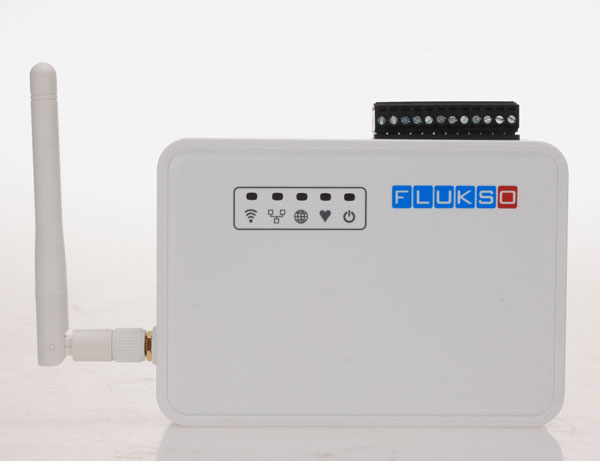
\includegraphics[width=0.4\textwidth]{flukso.png}}
	\caption{A \textit{Flukso} smart meter.}
	\label{fig:flukso}
\end{figure}

\subsection{Back end}
The server exposes REST web services to ensure synchronization, distribution and backup of energy consumption data. It also retrieves and distributes pricing information.

\subsection{Front end}
The \textit{Android} application displays data, provides solutions to different use cases and retrieves information such as energy price estimations at a given moment.

\subsection{Smart meter}
The device used in this project to monitor real-time energy consumption is called a \emph{smart meter}. It is an electronic device that records consumption of energy and communicates that information to a central system (see Figure \ref{fig:smartmeter_central}) \cite{Smartmeter:online}. In the case of electricity, it is placed close to the electricity meter of a house. A central system gives us access to the data collected.

\begin{figure}[htbp]
	\centerline{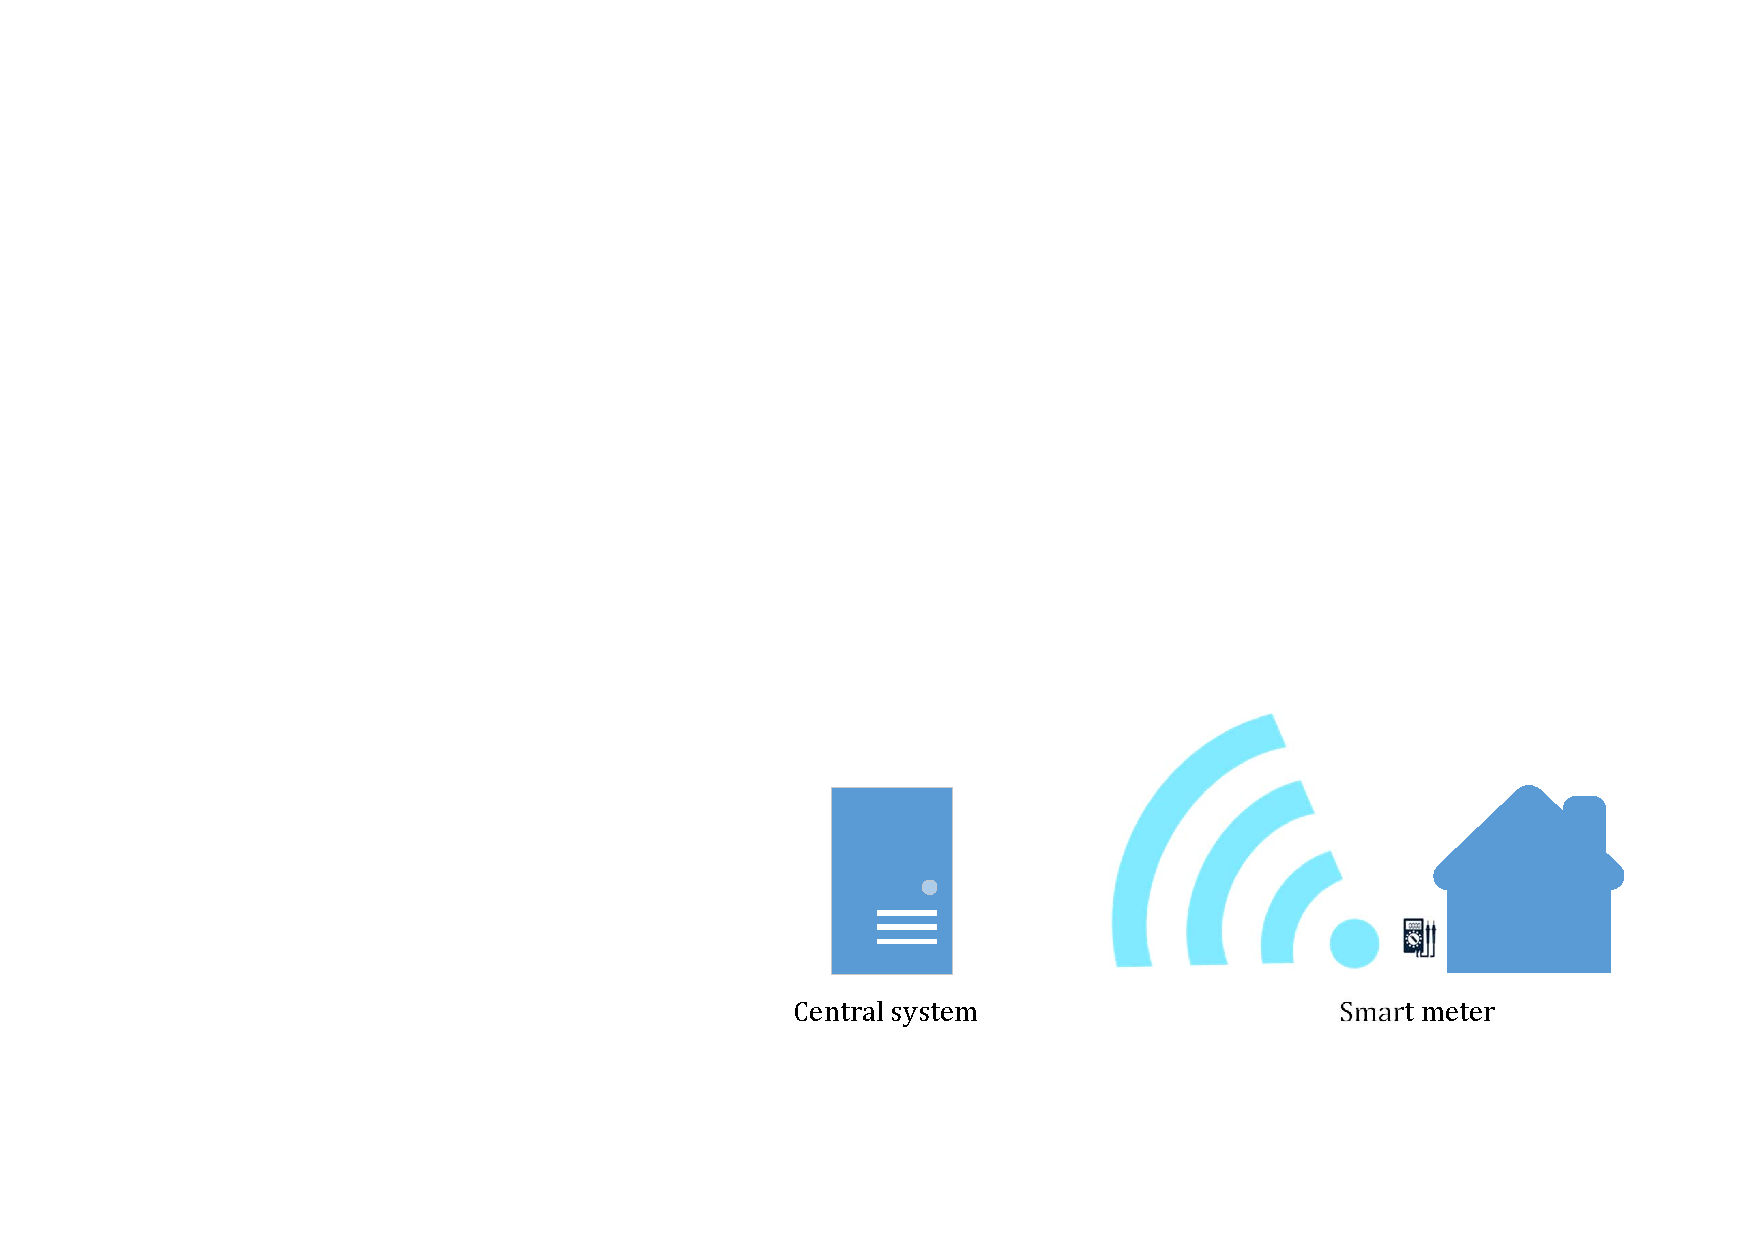
\includegraphics[width=0.6\textwidth]{smartmeter_central.pdf}}
	\caption{A smart meter with its central system.}
	\label{fig:smartmeter_central}
\end{figure}

\subsection{Open source}
As a part of a larger solution deployed by the company, the system had to be fully open source. Patrick Herbeuval, who worked on the same project last year, kindly gave us his consent to publish the code he wrote. For the first few months, we worked on a private \textit{Gitlab} repository. Then, in February, Vincent took the decision to move the code to \textit{Github} under the license Apache Version 2.0 \cite{Apache:online}. Everything is now available at \url{https://github.com/S23Y/}.\\

An open source project presented a great opportunity for me. Firstly, it means that the resultant code will not be limited to just a half a year of work as it may be useful to others someday. Indeed, contributions are encouraged by forking the repository, and contribute back using pull requests (see the \href{https://github.com/S23Y/myconsumption-android}{project’s readme on \textit{Github}}). Secondly, it allowed me to easily reuse other projects, libraries and components available on \textit{Github} (or elsewhere) thanks to the license of the project. Finally, playing with open source tools is a great way to discover and learn from the work of others.

\subsection{Positioning}
The way this project was defined and designed made it a unique solution. Nevertheless, the purpose of this work was not to make an application that controls electrical appliances. Instead, it aimed to \emph{visualize} and \emph{display} relevant information related to the \emph{monitoring} of energy consumption and, for that reason, represents only a part of the solutions described in the state of the art. As compared to those solutions, the real added value of \textit{MyConsumption} is that it is completely open source and based on recent technologies.

\section{The first version of MyConsumption}
We did not start this work from scratch. Last year, Patrick Herbeuval worked on the same subject during his master’s thesis \cite{patrick:thesis}. Here follows a description of the work he carried out.

\subsection{Back end}
The server designed by Patrick was built upon \textit{Spring}, an open source framework used to deploy web applications and to facilitate database access. The server allowed the collection of data from the smart meter API and subsequently kept them in the database. A full API was provided with the server, allowing different kind of access to the data it kept. A scheduled task ran in the background, retrieving the data every ten minutes from the manufacturer’s API.\\

One of the strengths of Patrick’s server was its modularity to add compatibility with other smart meters using a strong object-oriented approach. The following points weren’t addressed by him:
\begin{itemize}
	\item Security (i.e. authentication and secured communication with the server and its database);
	\item Push notifications to mobile devices;
	\item Processing and analysis of data (such as statistics);
	\item System deployment in practice (in a private or professional environment).
\end{itemize}

\subsection{Front end}
Patrick designed a small \textit{Android} application. As shown in Figure \ref{fig:patrick}, this client displayed a graph of the data received from the back end. It also featured a basic user login system and could handle the addition and deletion of sensors. The data fetched from the server were stored in a local database for offline visualization purposes. The following points weren’t addressed:
\begin{itemize}
	\item Receiving notifications from the server (such as an abnormal consumption alert);
	\item Analysis and evolution of data;
	\item System preferences;
	\item The security of the system and a strong authentication mechanism.
\end{itemize}

\begin{figure}[htbp]
	\centerline{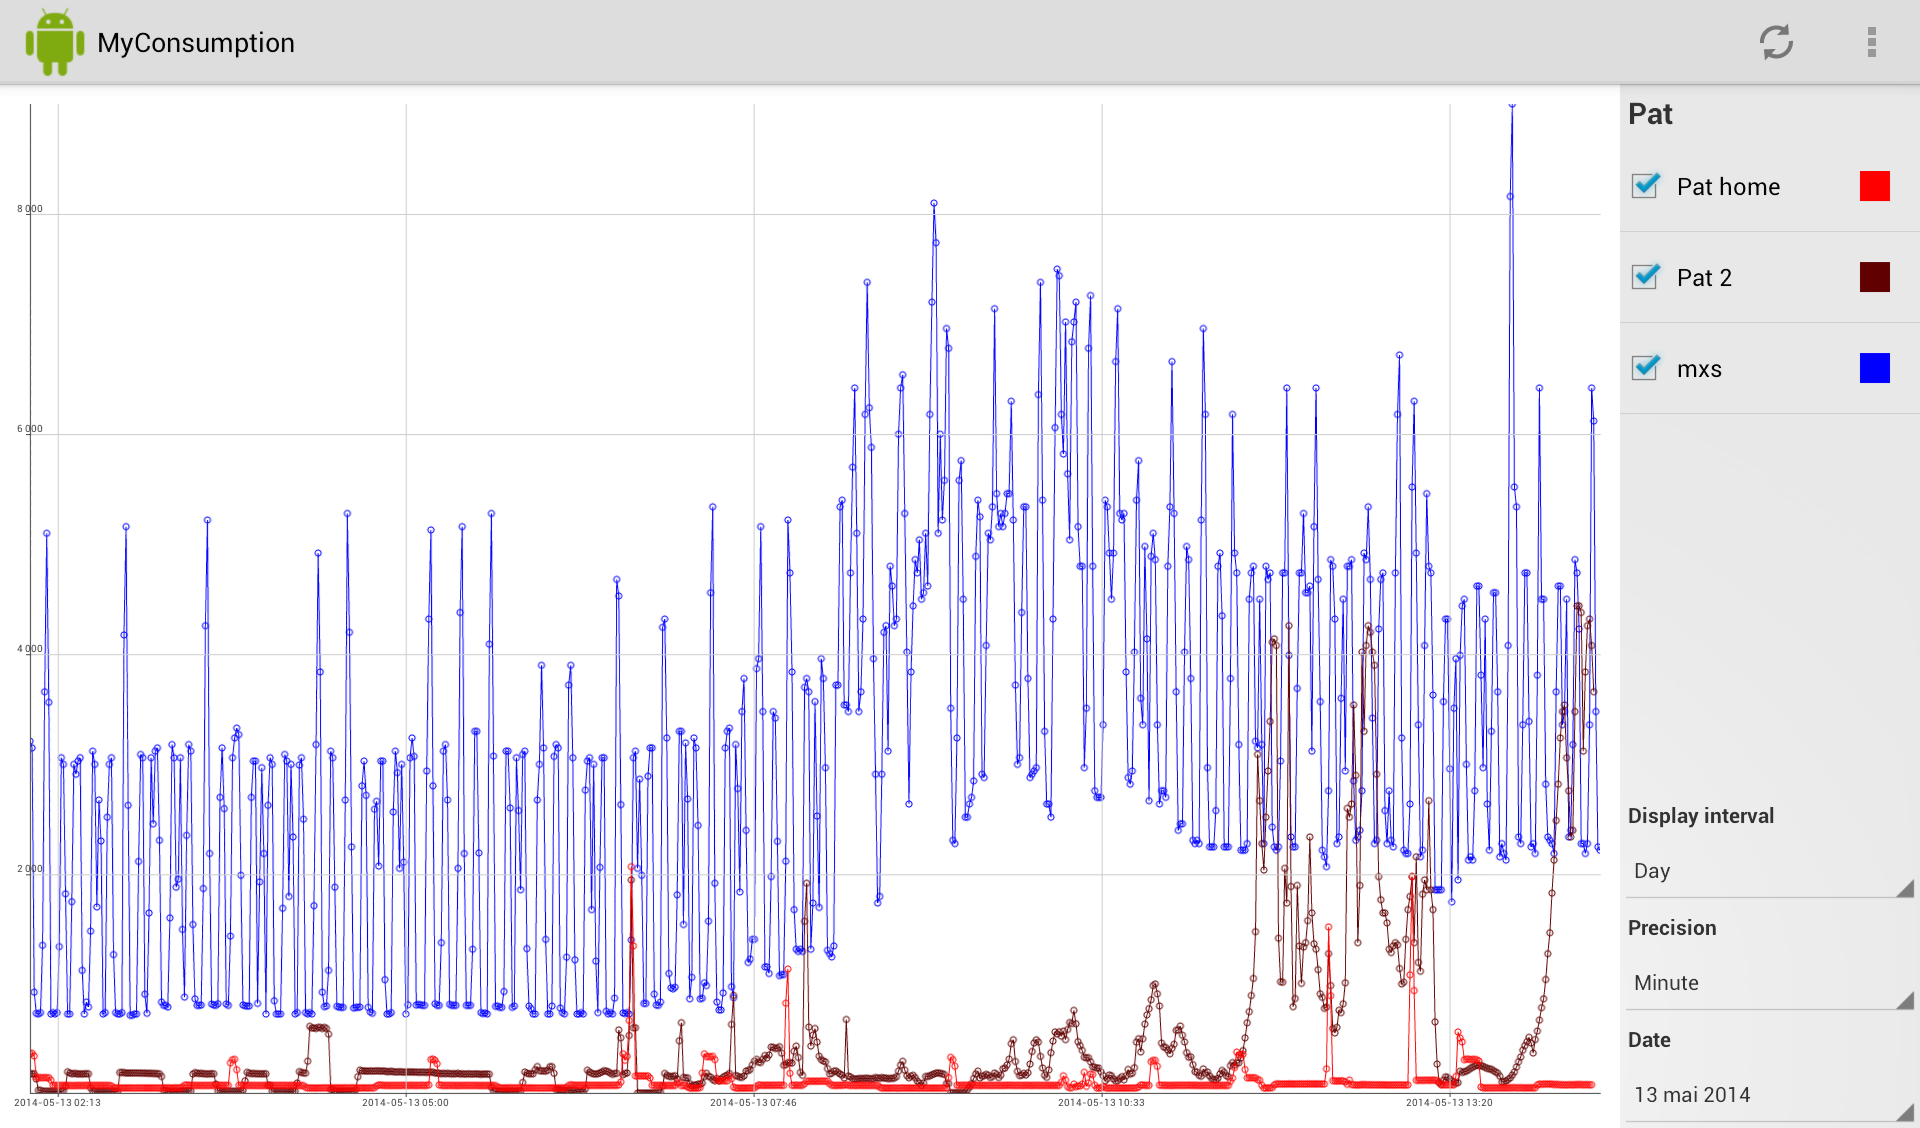
\includegraphics[width=0.85\textwidth]{patrick.png}}
	\caption{Main screen of Patrick’s application.}
	\label{fig:patrick}
\end{figure}

\section{Methodology}
With regard to the methodology, we followed an agile development approach. From August to May, a meeting was scheduled every two weeks. The first meetings with Antoine Smolders (computer scientist from the University of Liege working for A7 Software since 2013) and Vincent Keunen (CEO of A7 Software and co-founder and CEO of S23Y) allowed us to draw an overall sketch of the application and its desired requirements.  \\

After these initial meetings, we followed an iterative process. Every two weeks we discussed a feature to implement. The goal of the meeting was to arrive at a desired result that could be shown. Between the two meetings, we were able to design and implement this feature. In some ways, this process was similar to a very simplified scrum. During each meeting a report (see the Appendix) was made. It answered the following questions:
\begin{itemize}
	\item What have I done?
	\item What am I going to do?
	\item What causes difficulties?
	\item What questions have been raised?
\end{itemize}

This was also the perfect occasion to receive valuable feedback on the work carried out since the last discussion, and to prioritize the feature to implement next.

\newpage
\section{How to build and run the project}
Two dependency management systems are used in this project: \textit{Gradle} for the app and \textit{Maven} for the server. The following instructions explain how to use this work on a development machine.

\subsection{Mobile application}
\subsubsection{With Gradle and Android Studio}

The easiest way to build the app is to install \href{https://developer.android.com/sdk/index.html}{\textit{Android Studio}} v1.+ with \href{https://www.gradle.org/}{\textit{Gradle}} v2.+. You will need the \textit{Android} SDK API 21 and \texttt{my-consumption-api} available at \href{https://github.com/S23Y/myconsumption-server/}{\textit{Github} \textit{MyConsumption} Server} (run \texttt{mvn clean install} from the root directory of the server to install the API on your machine). Once installed, you can import the project into \textit{Android Studio:}
\begin{enumerate}
	\item Open File;
	\item Import Project;
	\item Select \texttt{build.gradle} under the project directory;
	\item Click OK.
\end{enumerate}

\subsubsection{Release}
Copy the \texttt{.apk} on an \textit{Android} device and install it (installation of apps from unknown sources must be allowed in your settings). Our \texttt{.apk} file is available at \url{http://bit.ly/myconsumption}.

\subsubsection{Test user}
A user which owns two sensors is available to test the application with the following credentials:
\begin{itemize}
	\item username: \texttt{thib}
	\item password: \texttt{thib}
\end{itemize}

\subsection{Server}
\subsubsection{With Maven}
The easiest way to build is to install \href{http://maven.apache.org/download.html}{\textit{Maven}} v3.+ in your development environment. 
Then, the build is pretty simple:
\begin{itemize}
	\item Run \texttt{mvn clean install} from the root directory. 
\end{itemize}

\subsubsection{Deployment}
The deployment of the server is described in the Appendix of this document.

\section{About the company}
Software Services For Energy (S23Y) is dedicated to providing innovative software services to the energy sector, worldwide \cite{S23Y:online}. They launched the \textit{StarfishRespect} open source platform to allow all energy concerned companies to innovate together and create a vibrant ecosystem. \textit{StarfishRespect} is based on the innovative software platform built for Lampiris by Manex (Belgium). 

\begin{figure}[htbp]
	\centerline{
\includegraphics[width=0.4\textwidth]{logo_s23y.png}}
	\caption{The S23Y logo.}
	\label{fig:logo_s23y}
\end{figure}

\part{Design}
\renewcommand\partcontent{DESIGN: }

\chapter{Overview}
Before defining features, use cases and user interfaces we set out to implement, this section provides a high-level view of the system and introduces the tools involved in its conception. The interactions between each part of the system are also outlined. The purpose of this section is not to go into great detail, but rather to explore how the software works in a summarized form. The following chapters will describe its implementation and provide further information.

\section{Architecture}
The Figure \ref{fig:global} illustrates how each part interacts with the others. From this diagram, we see that various actors are involved:
\begin{itemize}
	\item The \textit{Android} Application, which communicates with its local database (\textit{SQLite}), with our server and with the \textit{Google Cloud Messaging} server;
	\item Our server\footnote{The server is available at \url{http://myconsumption.s23y.com}.}, which is built upon \textit{Spring Boot}. It provides RESTful services as well as a Java API. It communicates with its local database (\textit{MongoDb}), with the smart meter API and with the \textit{Google Cloud Messaging} server;
	\item The smart meter manufacturer API, which allows access to their data;
	\item The \textit{Google Cloud Messaging} server.
\end{itemize}

\begin{figure}[htbp]
	\centerline{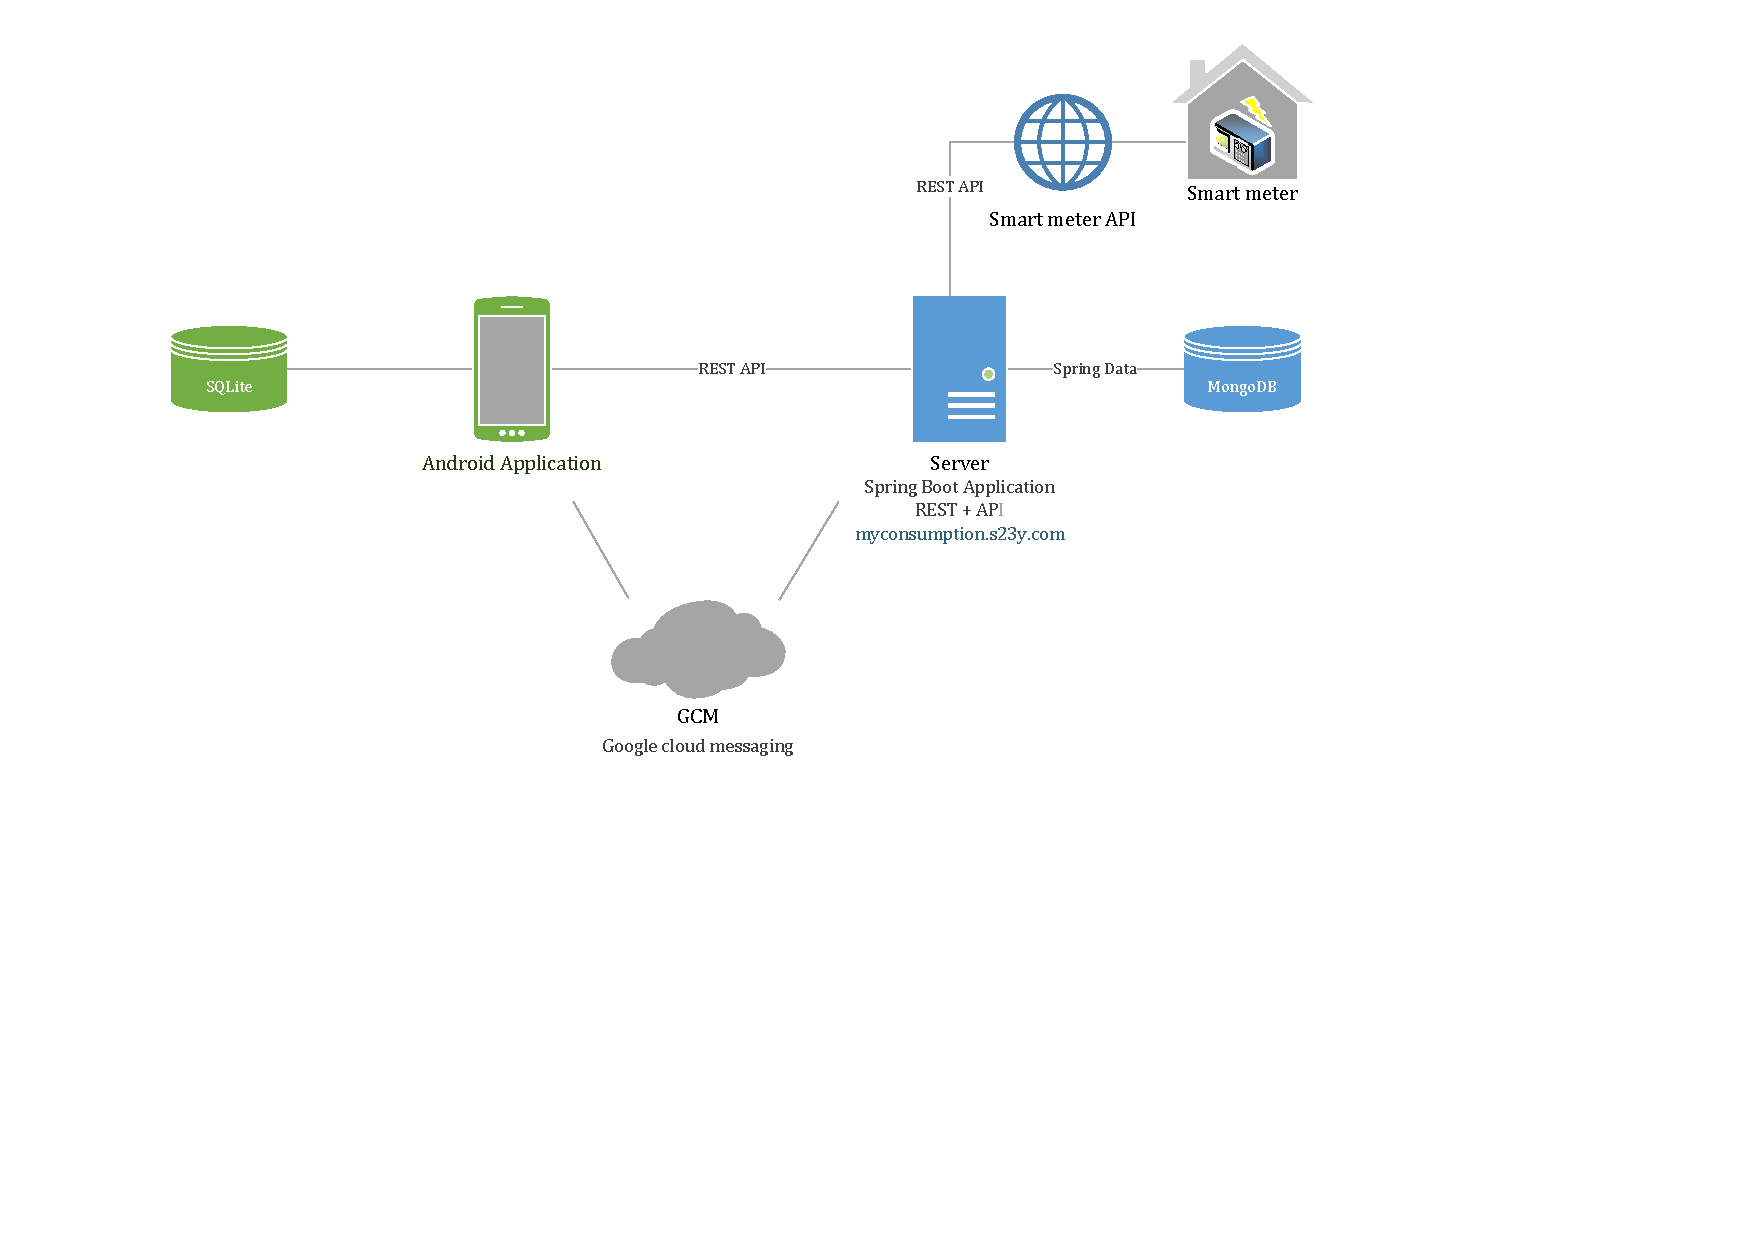
\includegraphics[width=1\textwidth]{global.pdf}}
	\caption{An overview of the system.}
	\label{fig:global}
\end{figure}

\section{Tools involved}
The main tools and concepts related to the mobile application and the server are described below. Some of them may already be well-known to readers, but since they will be used in the following chapters of this work, we thought it relevant to include every definition in the two following sections.

\subsection{Server}
\subsubsection{IntelliJ IDEA}
The Java Integrated Development Environment (IDE) used during this work was \textit{IntelliJ IDEA}. It was developed by JetBrains (formerly known as IntelliJ), and is available as an Apache 2 Licensed community edition, and in a proprietary commercial edition \cite{intellij:online}. It is a good software for enterprise, mobile and web development and it integrates well with all the latest modern technologies and frameworks described below.

\subsubsection{Spring and Spring Boot}
\textit{Spring} is an open source application framework for the Java platform. It supplies many useful features, such as Inversion of Control, Dependency Injection, abstract data access, transaction management, and more \cite{professional:book}. It was conceived in 2002 in response to industry complaints that the Java EE specification was sorely lacking and very difficult to use.\\

The server designed for \textit{MyConsumption} was first built upon \textit{Spring}, to easily deploy RESTful web services and to facilitate the database access. During the course of this work, we updated the server from \textit{Spring} to \textit{Spring Boot} to ease its configuration. \textit{Spring Boot} makes it easy to create stand-alone, production-grade \textit{Spring} based applications that you can “just run” \cite{Springboot:online}. \textit{Spring Boot} is a more recent tool, released in 2013.\\

The reasons behind the choice of \textit{Spring Boot} are the following. Firstly, it supports \textit{Spring} and the first version of the server available. Secondly, it is an open source framework well integrated with Java applications that perfectly suits the needs of the back end described above. Finally, the employees of S23Y have a deep knowledge of \textit{Spring} and were able to guide me through the learning process of its use. \\
Several modules of \textit{Spring Boot} were used in the project:
\begin{itemize}
	\item \texttt{spring-boot-starter-web}: to deploy the RESTful services;
	\item \texttt{spring-boot-starter-tomcat}: for the deployment on a \textit{Tomcat} server;
	\item \texttt{spring-boot-starter-security}: to add a layer of security;
	\item \texttt{spring-boot-data-mongo}: to provide an integration with the \textit{MongoDb} document database.
\end{itemize}

\subsubsection{Smart meter API}
Flusko, the smart meter used to collect the data, deploys an API available at \url{https://api.flukso.net/sensor}. A module of our server was dedicated to fetch data from their API and to store them in our own database.

\subsubsection{Google Cloud Messaging}
The \textit{Google Cloud Messaging} (GCM) service for \textit{Android} made it possible to send data from our server to specific users’ \textit{Android}-powered device \cite{googlecloudmsg:online}. The GCM service handles all aspects of queueing of messages and delivery to the target \textit{Android} application running on the target device. It is the standard system in \textit{Android} to implement push notifications and therefore  appeared to be the best option.

\subsubsection{MongoDb}
The choice of \textit{MongoDb} as a database of the server was made and motivated last year by Patrick during his master’s thesis.\\

\textit{MongoDb} is a NoSQL cross-platform document-oriented database. It is not structured around the traditional table-based relational model. Instead, JSON-like documents with dynamic schemas (called BSON) are used \cite{Mongo:online}. These documents have the advantage of making the integration of data in certain types of applications easier and faster. 

\paragraph{NoSQL databases}
The original call for the term “NoSQL” asked for “open source, distributed, non-relational databases” \cite{nosql:book}. But there is no formal definition of NoSQL databases. Still, they do have some common characteristics:
\begin{itemize}
	\item They do not use the relational model;
	\item They run well on clusters;
	\item Most of them are open source;
	\item They are built for the 21st century web estates;
	\item They are schemaless.
\end{itemize}

\paragraph{Why are NoSQL databases interesting?}
The first reason is because a great deal of application development effort is spent on mapping data between in-memory structures and a relational database. A NoSQL database may better fit the application’s needs, and simplify that interaction. The second reason concerns large-scale data. This project may need to support large volumes of data as it aims to keep track of the consumption of many clients. However, as companies capture more and more data, they also want to process it more quickly. With clusters and NoSQL database explicitly designed for this purpose, there is a better fit for big data scenarios. Moreover, it has the advantage to use smaller and cheaper machines.

\subsection{Mobile application}
\subsubsection{Android}
\textit{Android} is a mobile operating system based on the Linux kernel and currently developed by Google \cite{Android:online}. Its interface is designed for touchscreens with a mobile vision. At the time of writing, it is the most popular mobile OS with hundreds of millions of mobile devices in more than 190 countries around the world \cite{Androidlollipop:online}. Furthermore, it is growing fast: every day another million users start to use a new device for the first time. The first version was released six years ago, in 2008. Today, the latest release is \textit{Android} 5.1.1 Lollipop (April 21, 2015). The system is more and more integrated with various Google Services such as Maps, Google+ etc.

\subsubsection{The Android SDK and Android Studio}
One of the goals of Google, via \textit{Android}, is to create a great community of developers. In order to do so, they provide them a Software Development Kit (SDK) that includes sample projects with source code, development tools, an emulator, and libraries required to build \textit{Android} applications. \\

Another great tools for developers is \textit{Android Studio}, the official IDE for \textit{Android} application development, based on \textit{IntelliJ IDEA} \cite{Androidstudio:online}. It is the IDE used to implement this work.

\subsubsection{Support library}
Besides the SDK, developers have access to the \textit{Android Support Library}. This is a set of code libraries that provide backward-compatible versions of \textit{Android} framework APIs \cite{Support:online}. It means that applications can use the libraries' features and still be compatible with devices running \textit{Android} 1.6 (API level 4) and up. One of our goals with \textit{MyConsumption} is to support a large set of devices, which is the reason why we used the \textit{Support Library}.

\subsubsection{Google Play Services}
The goal of the \textit{Google Play Services} is to allow every application to take advantage of the latest Google-powered features. It includes the update system from the \textit{Google Play Store} and other integrations with the Google ecosystem. We used the \textit{Play Services} with the notifications system.

\subsubsection{SQLite and ORMLite}
As its name suggests, \textit{SQLite} is a light relational database management system. In contrast to many others, it is not a client-server database engine: it is self-contained and serverless \cite{SQLite:online, SQLite2:online}. \textit{SQLite} is fully integrated with \textit{Android} within the package \texttt{android.database.sqlite} which makes its adoption easy.\\

\textit{ORMLite} is a tool used alongside \textit{SQLite}. We chose this tool because it provides lightweight functionalities for persisting Java objects to SQL databases \cite{OrmLite:online}. By adding Java annotations to a class, one can store an instance directly in \textit{SQLite}.

\subsubsection{\textit{Spring} for \textit{Android}}
As the \textit{Spring} framework is used on the server side, a good solution to communicate with it is to use \textit{Spring} for \textit{Android}. This is a framework that is designed to provide components of the \textit{Spring} family of projects for use in \textit{Android} applications \cite{Springandroid:online}.


\chapter{Features, interfaces and use cases}
The design process kept us busy for some time, since it was important to think in depth about the core-features of the application before implementing them. A noteworthy point is that all the features described below were designed with the need for off-line synchronization in mind. 

\section{Features to implement}
One of the first questions that we tackled was: “what could the relevant features of this app be?”.  The following answers were discussed during the meetings. 

\subsection{Graph smoothing}
In the beginning of the project, the application was only able to display a graph of the consumption. As you can see in Figure \ref{fig:chart_high_peaks}, the screen is not really readable due to the high peaks. Allowing the user to smooth the graph with an adjustable slider was thought to be a potentially interesting feature. Based on the data, an easy correction could be calculated for each sample by means of a linear interpolation. 

\begin{figure}[htbp]
	\centerline{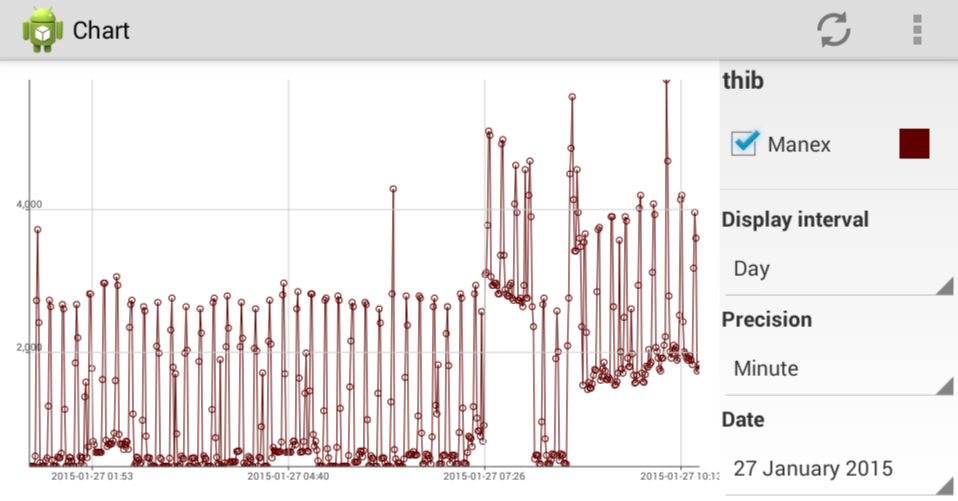
\includegraphics[width=0.6\textwidth]{chart_high_peaks.png}}
	\caption{The graph is not easy to read.}
	\label{fig:chart_high_peaks}
\end{figure}

\subsection{Provide an analysis of energy consumption based on statistics}
We thought that, given a period (day, week, month, year...), a user should be able to see an analysis of their consumption. For example, information about peak and off-peak consumption\footnote{The term peak consumption is the English equivalent of “\textit{électricité de jour}” while off-peak consumption means “\textit{électricité de nuit}”.}, average consumption, extrema etc. could be useful.

\subsection{Savings between periods}
This feature is related to the previous one. Based on the idea that we would retain information about a given period, it could be interesting to see the savings (or the losses) made between two periods. For example, one could see how and why the amount of an energy bill is significantly dropping.

\subsection{Compare one’s consumption to a given consumer profile}
Couples, average household, big families... All these different profiles have varying bills at the end of the month. It could be interesting for an individual user to see how (s)he compares with standard profiles.\\

The consumer profile should be relevant enough to be significant for the user. One idea was to take localization into account (since you do not have the same consumer profiles in every country). Another idea was to build those profiles based on public \textit{Flukso} data. 

\subsection{Evolution of consumption}
A user’s consumption could be impacted by a change of habit or behavior (for example, buying a new dishwasher). One idea was to allow the user to enter a comment on the graph at a given time. With this feature, (s)he could see the advantage associated with that new acquisition. Another feature suggested was to estimate the energy consumption and cost at the end of a period (e.g. a month) by extrapolation.

\subsection{Manual consumption reading}
To target people who do not have a smart meter, it could be useful to enter consumption data manually. However, it is not very likely to see someone using the mobile application this way in a day-to-day usage.

\subsection{Alerts and abnormal cases}
For example, if the consumption is starting to increase in an abnormal way, the system could draw the user’s attention to this fact. Any problem related to the connection between the back end and a smart meter should also be reported.

\subsection{Retrieving and distributing pricing information}
The back end needed to receive electricity price data in some way. A public API could help us to tackle this problem. Moreover, the application should use this information to display the cost associated with the energy consumption over a given period.

\section{User interfaces and mockups}
The second step in the design process was to think about user interfaces by drawing \emph{mockups}\footnote{A \emph{mockup} is a prototype of a design used for demonstration purposes.}. The application offers different screens which were discussed during the meetings. Several of them, such as the login screen, are based on a previous version of the mobile application, and will not be discussed here.

\subsection{Main screen}
The main screen of the application is the one which displays the graph. It is composed of a line chart of the user’s consumption and a panel with options to choose sensors, intervals and dates. Although it is largely based on a previous version of the application, several parts have been improved: the integration with the rest of the application; the toolbar; the display of the options on smaller screens; and the smoothing slider. The mockup is shown in Figure \ref{fig:chart_activity_mockup}. Notice the reload button in the upper right corner.

\begin{figure}[htbp]
	\centerline{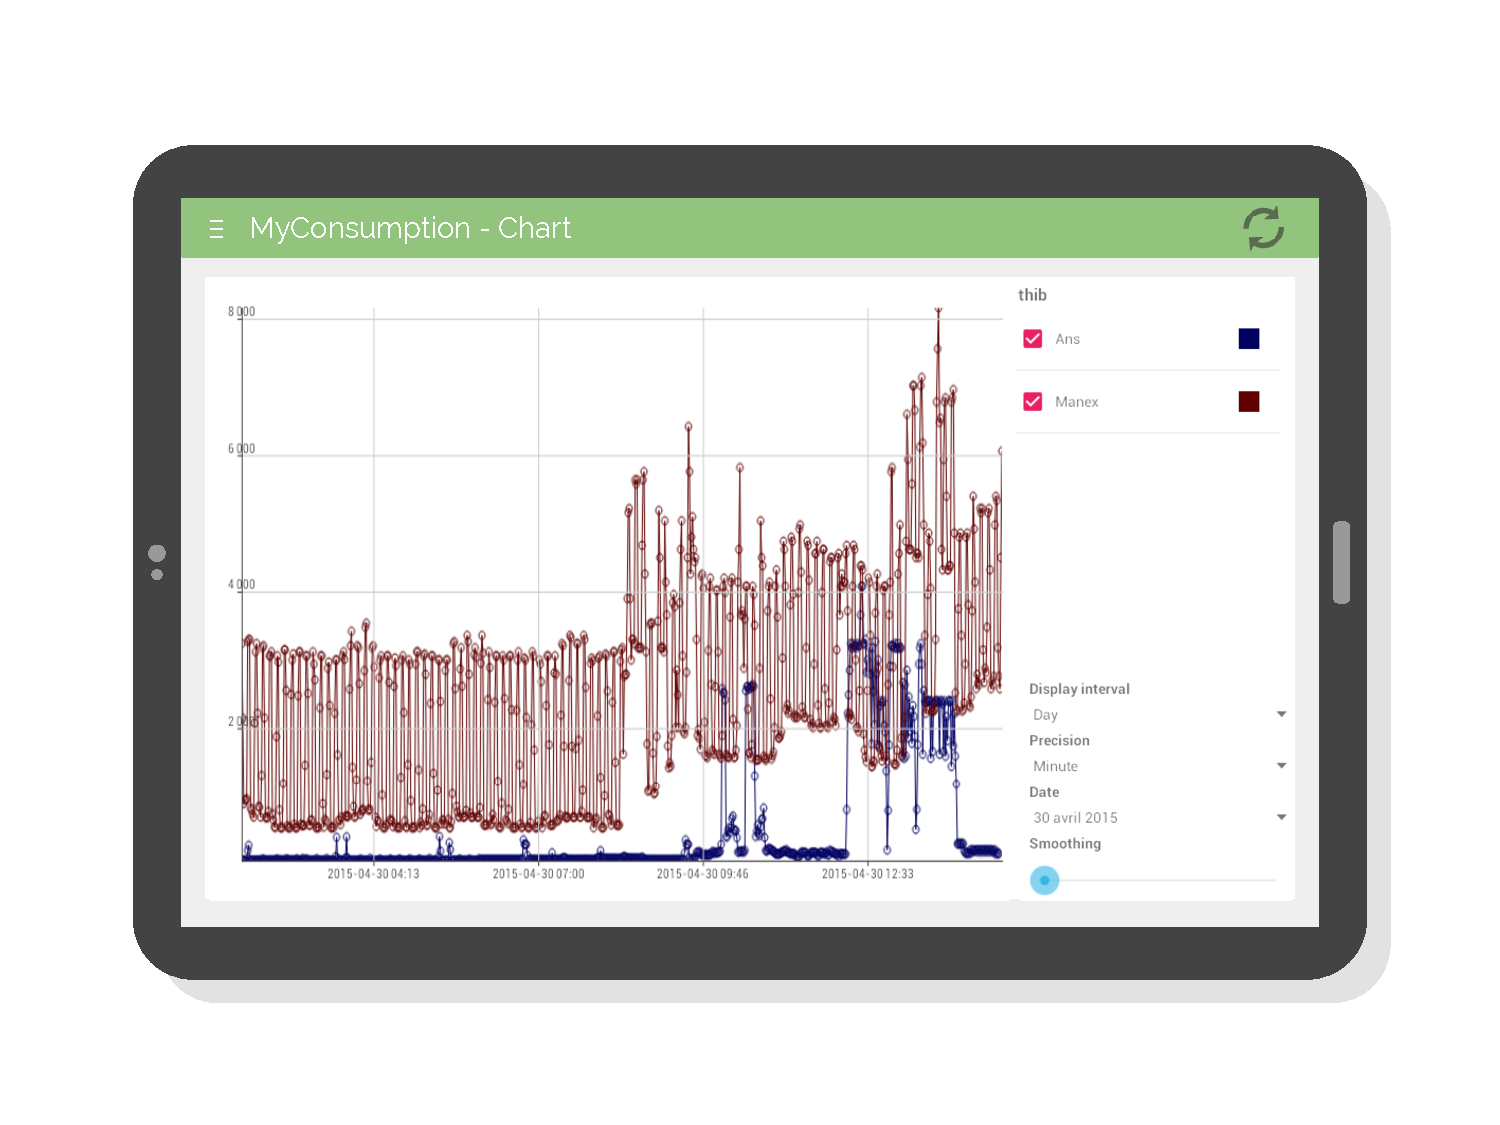
\includegraphics[width=0.85\textwidth]{chart_activity_mockup.pdf}}
	\caption{The mockup of the main screen of the application with two sensors.}
	\label{fig:chart_activity_mockup}
\end{figure}

\subsection{Statistics}
The second screen we discussed displays the statistics. The challenge here was to provide a lot of information on the same screen. Different colors and a graph were used to draw the user attention to key points. As several periods are needed, the idea was to use tabs to display them easily. To switch between sensors, a drop-down menu was added to the toolbar. The mockup is given in Figure \ref{fig:stat_activity_mockup}.\\

As far as the statistical items\footnote{Note that it is important to differentiate the units associated with the statistics. Kilowatt-hours, or kWh, is an \emph{energy} unit which describes the \emph{total amount} of electricity used or produced over a period of time. Watts, or W, is a \emph{power unit} which describes the \emph{rate} of using or producing electrical energy (or how much is being used right now).}  are concerned, we thought it was relevant to include:
\begin{itemize}
	\item The consumption over the period (kWh);
	\begin{itemize}
		\item The associated cost in \euro;
		\item The associated environmental footprint (in kg of \(CO_2\));
	\end{itemize}
	\item The difference between the consumption over this period and the last one (kWh);
	\item The average consumption (W);
	\item The maximum and minimum values (W);
	\item The consumption during high peaks (over the day (kWh)) and off-peaks (over the night (kWh)).
\end{itemize}

\begin{figure}[htbp]
	\centerline{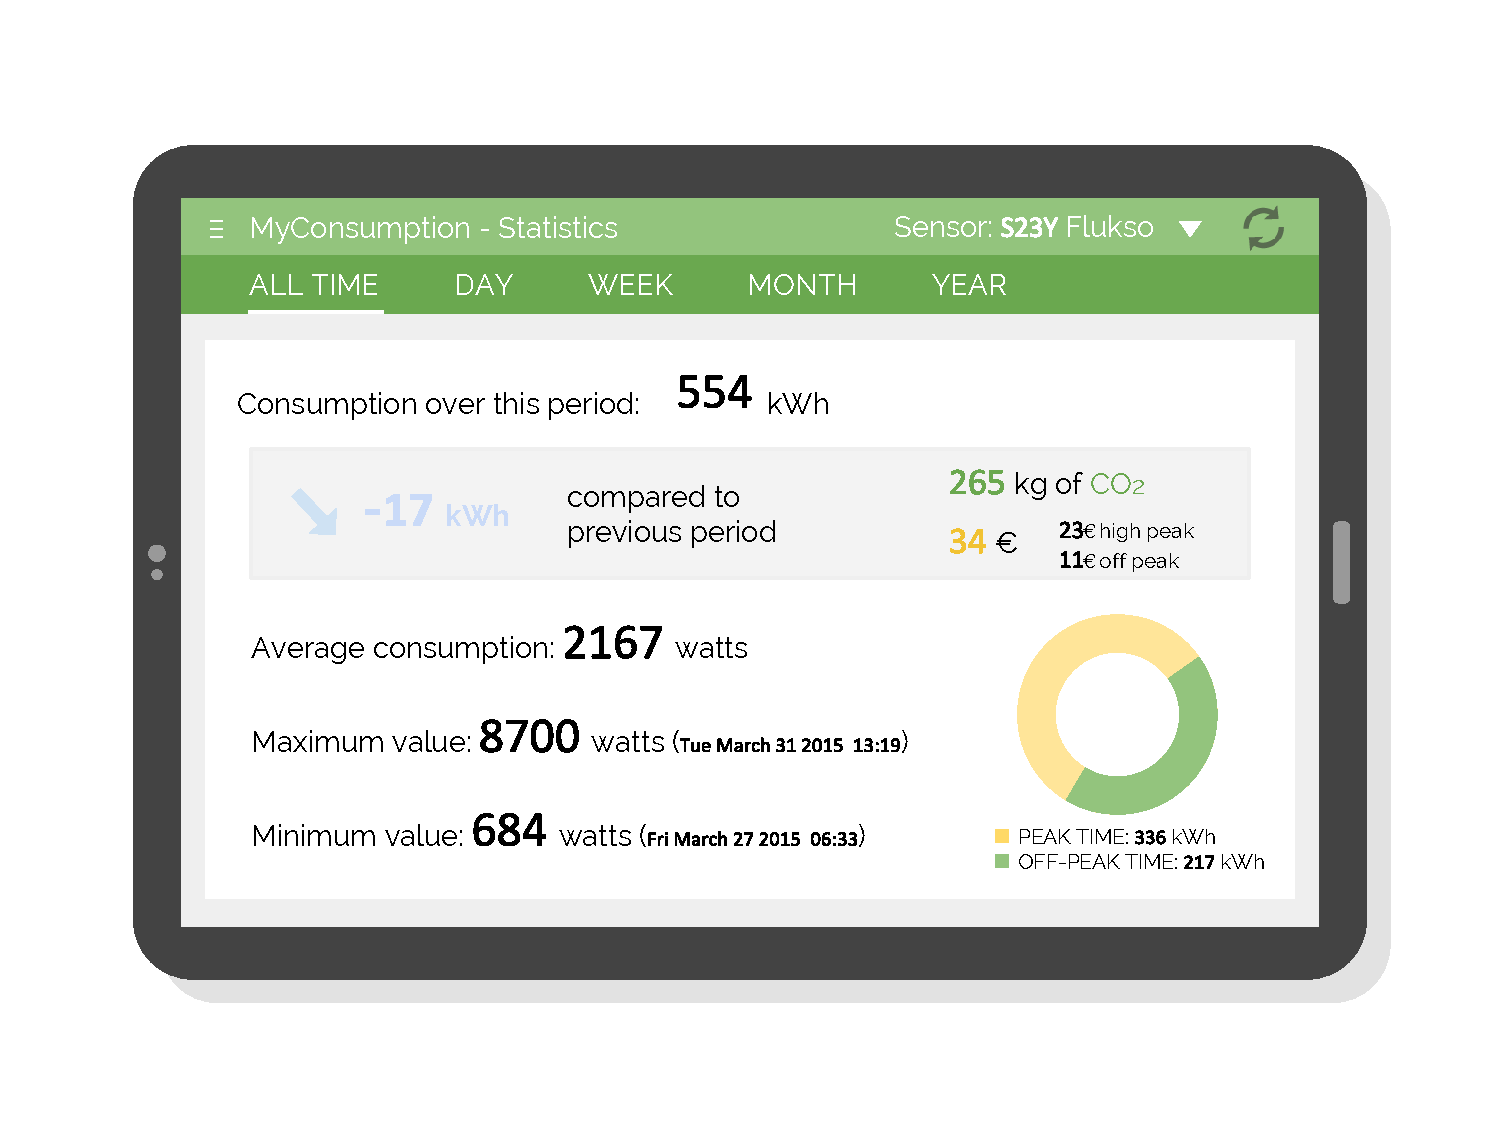
\includegraphics[width=0.85\textwidth]{stat_activity_mockup.pdf}}
	\caption{The mockup of the statistics screen.}
	\label{fig:stat_activity_mockup}
\end{figure}

\subsection{Profile comparison}
As discussed above, a relevant feature we identified was for a user to be able to compare their consumption to a standard profile. At the early discussion stage of the work, we did not know how the standard profiles would be computed. This uncertainty is the reason why the mockup proposed in Figure \ref{fig:comparison_activity_mockup} is quite simple. It is composed of:
\begin{itemize}
	\item A recall of the description of the standard profile selected and a button to modify it;
	\item A little comparison between the real consumption and the one of a standard profile;
	\item A graph that highlights the difference between the standard profile and the current consumption.
\end{itemize}

\begin{figure}[htbp]
	\centerline{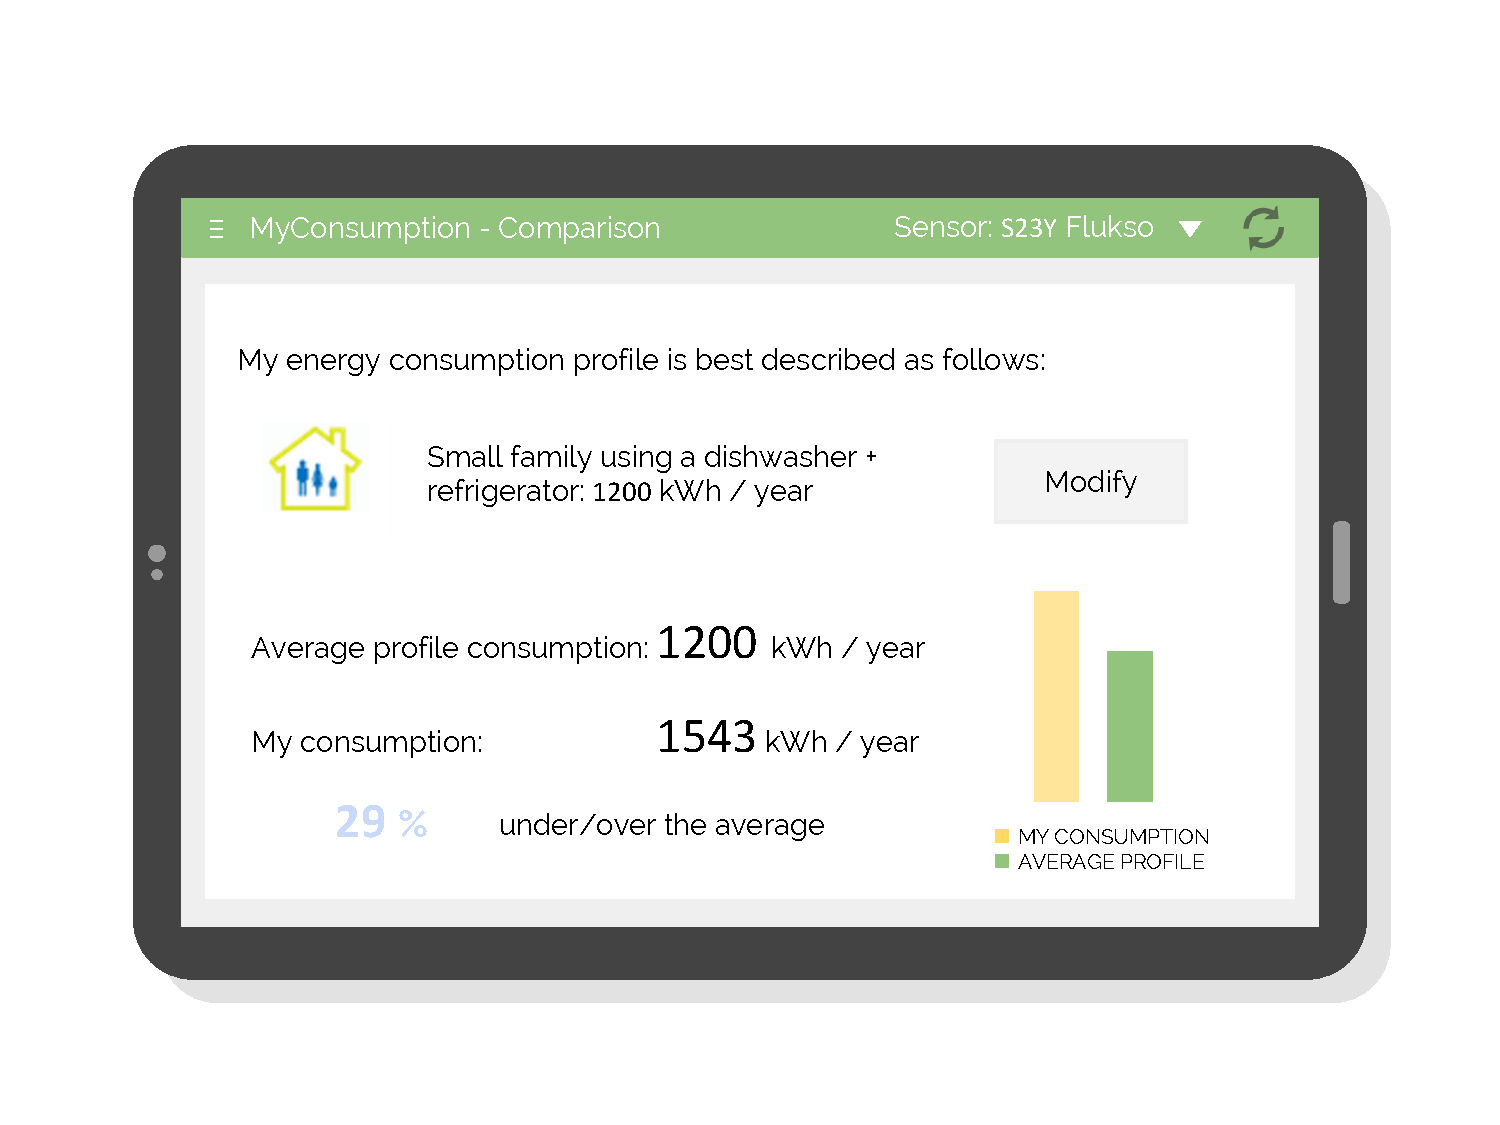
\includegraphics[width=0.85\textwidth]{comparison_activity_mockup.pdf}}
	\caption{The mockup of the comparison screen.}
	\label{fig:comparison_activity_mockup}
\end{figure}

\subsection{Settings}
Last but not least, a settings screen will allow one to specify different preferences. For example, a user could see a possibility to receive notifications from the server, select their standard consumption profile, enter their annual consumption if (s)he knows it... A description of this screen is given in Figure \ref{fig:settings_activity_mockup}.

\begin{figure}[htbp]
	\centerline{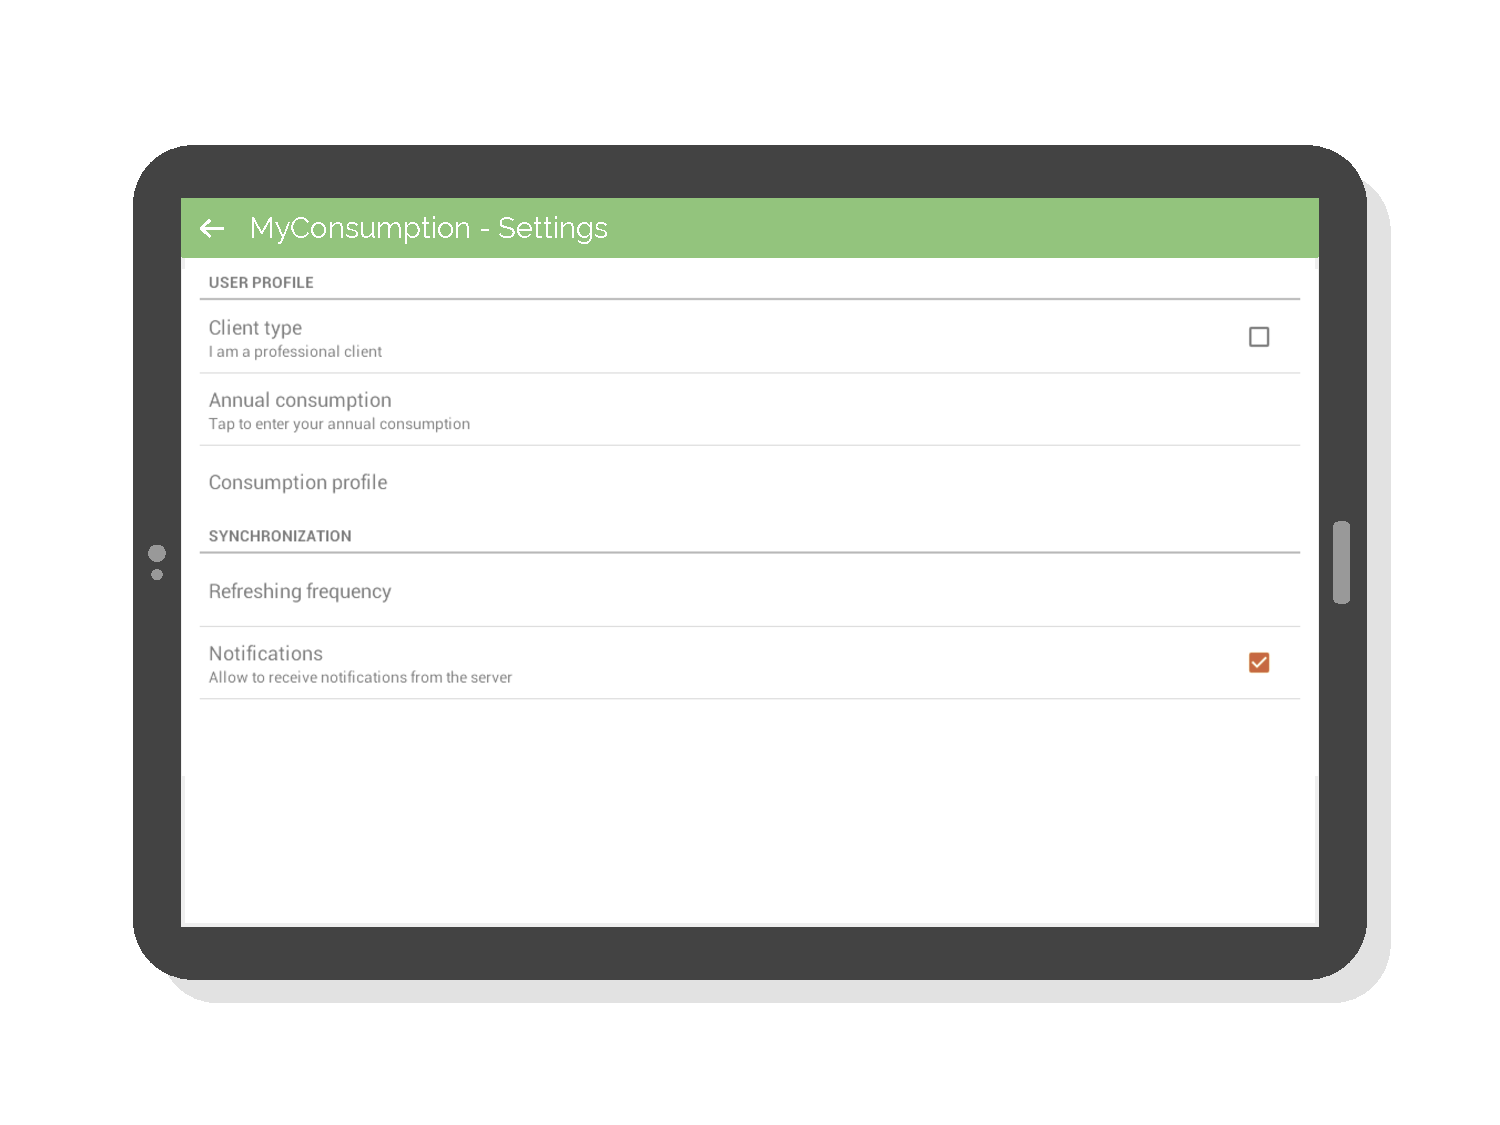
\includegraphics[width=0.85\textwidth]{settings_activity_mockup.pdf}}
	\caption{The mockup of the settings screen.}
	\label{fig:settings_activity_mockup}
\end{figure}

\newpage
\section{Defining use cases}
As a use case represents a typical interaction between a user and the system \cite{boigelot}, not all the features discussed below will be addressed in this section. The use cases defined here correspond to high-level goals and are described as if a virtual camera was filming interactions between the system and its users.\\

\subsection{Log in to the application}
\begin{table}[h!]	
	\centering
	\begin{tabular}{|p{2cm}|p{8cm}|} \hline
		Actor	 	& User \\ \hline
		Goal	 	& Accessing the application by providing a username and password. \\ \hline
		 Overview	& 

		 The User starts the application and a form requests them to  enter their credentials. If the User has no credentials, an option is available to him/her to create a new account by entering a name and a password. When those credentials are provided on the login screen, the User clicks on a button to access the app. The main screen is then displayed. If the credentials do not match any user, a message is displayed asking the User to reenter them. \\ \hline
	\end{tabular}
	\caption{Log in to the application.}
\end{table}

\newpage
\subsection{Switch between screens}

\begin{table}[h!]	
	\centering
	\begin{tabular}{|p{2cm}|p{8cm}|} \hline
		Actor	 	& User \\ \hline
		Goal	 	& Switching from the current screen to another one.
\\ \hline
		 Overview	& 
		 The User is on a screen of the application. By pushing an icon on the upper left corner of the screen or by sliding from the left of the screen to the center, a sliding panel is shown. This panel offers to the User the option to choose a new screen to display. By clicking on one of them, the current screen is replaced by this one and the sliding panel disappears.
\\ \hline
	\end{tabular}
	\caption{Switch between screens.}
\end{table}

\subsection{Smooth the graph}

\begin{table}[h!]	
	\centering
	\begin{tabular}{|p{2cm}|p{8cm}|} \hline
		Actor	 	& User \\ \hline
		Goal	 	& Smoothing the graph to make it clearer.
\\ \hline
		 Overview	& 
		 The User is on the main screen of the application which displays a graph of his/her consumption. The User uses a slider to set a smoothing value. When the value is set, the graph is updated.
\\ \hline
	\end{tabular}
	\caption{Smooth the graph.}
\end{table}

\subsection{Reload the data}

\begin{table}[h!]	
	\centering
	\begin{tabular}{|p{2cm}|p{8cm}|} \hline
		Actor	 	& User \\ \hline
		Goal	 	& Reloading the data from the server.
\\ \hline
		 Overview	& 
		 The User is on the one of the screens of the application which displays the data. The User clicks the reload button on the right upper corner of the screen. The system replaces the current data with a reloading animation. When the reload is complete, the new data appear.
\\ \hline
	\end{tabular}
	\caption{Reload the data.}
\end{table}


\chapter{Security}
For some mobile applications security might not be an issue, but in our case we are dealing with sensitive information. Indeed, if a burglar could access the energy consumption reports of a given house, (s)he could determine whether people are present in the building or not, making theft far easier. \\

The mechanism that determines whether someone has access to a system is called \emph{authorization} \cite{professional:book}. This process is closely related to \emph{authentication}, which is always the first step in \emph{authorization}: Bob may be \emph{authorized} to view some confidential files of a company, but until he is \emph{authenticated}, the system cannot be sure that this person is really Bob (and if he is not, he should not be \emph{authorized} to access the files). \\

This chapter aims to address both \emph{authorization} and \emph{authentication} issues related to \textit{MyConsumption}. Solutions are discussed for each specific security concern in the different parts of the system.

\section{The first version of MyConsumption}
The first version of the mobile application had a simple mechanism of username-password authentication: to authenticate and establish his/her identity, the user must enter their username and password when prompted. However, this password was used only on client side to authenticate. Additionally, it was sent in plain text over the internet to the server where it was likewise stored as plain text.\\

Moreover, the RESTful service had no security mechanism. Every resource was accessible to anyone and the exchanges were unencrypted. Finally, no credentials were provided with the \textit{MongoDb} server, meaning that anyone who could access the same network as the server could also access all data it contains.

\section{Different authentication mechanisms}
To add a layer of security to the system, different possibilities were offered to us. Before describing our implementation, this section describes the various options at hand. It is based on the Part 4: “Securing Your Application with Spring Security” of the book “Professional Java for Web Applications” \cite{professional:book}.

\subsection{Basic authentication}
This HTTP authentication protocol enables both authentication requests and authentication challenge responses. To access a resource protected by basic authentication, the username and password are provided and encapsulated in a request with an authorization header that contains the key-word \texttt{Basic} followed by the Base64-encoded credentials:

\begin{lstlisting}[breaklines]
	GET /support HTTP/1.1
	Host: www.s23y.org
	Authorization: Basic Sm9objpncmVlbg==
\end{lstlisting}

\subsubsection{Vulnerabilities}
Because Base64 is only an encoding algorithm, the credentials are sent in plain text and vulnerable to sniffing. Attackers can access username and password, but also protected resources. This issue can be circumvented by using HTTPS requests (which protects the credentials from snooping (man-in-the-middle) and prevents replay attacks).\\

Another vulnerability is added if the password is stored in plain text on the server side. However, modern web servers provide mechanisms for storing passwords using one-way hashes.

\subsection{Digest authentication}
Where HTTPS is either not an option or not wanted, a digest access authentication can achieve a certain level of security over HTTP using MD5 checksum algorithm with two different nonces (one nonce for the server and one for the client) and a serial request number (to prevent replay attacks). The password is kept secure as it is never sent over the network and it is stored in hashed format.\\

Nevertheless, due to recent attacks on MD5, which is now largely obsolete, digest authentication is generally not a security mechanism one should rely on anymore, outside of the security of HTTPS. And even over HTTPS, it is recommended to still use digest over basic when possible.

\subsubsection{Client certificate authentication}
This is one of the most secure authentication protocols, even if it involves no username or password. It requires HTTPS. The server communicates with the client using public/private key pairs. On the client side, the private key is securely generated and stored on the machine.\\

The disadvantage of this protocol is that it requires the user to hold a little IT knowledge and users cannot easily use a different computer to authenticate. Nevertheless, it has the huge advantage that credentials cannot easily be compromised. 

\subsubsection{Claims-based authentication}
This mechanism uses a trusted third-party application to authenticate users. For example, one can use Facebook to authenticate to another site.\\

As shown in Figure \ref{fig:claimed}, when a user attempts to access a protected resource, (s)he is redirected to the third-party application. After successful authentication, (s)he can access the resource with a claim asserting his/her identity. Many different protocols, such as OAuth and SAML, implement this type of authentication.

\begin{figure}[htbp]
	\centerline{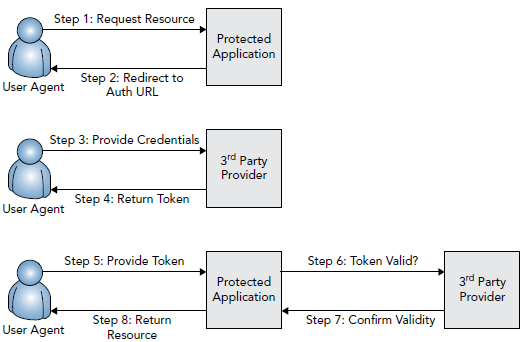
\includegraphics[width=0.7\textwidth]{claimed.png}}
	\caption{Claims based authentication \cite{professional:book}.}
	\label{fig:claimed}
\end{figure}

\subsubsection{Multi-factor authentication}
All the protocols mentioned so far only provide one authentication factor. As its name suggests, multi-factor authentication requires the user to perform several steps to identify, making its security advantages significant.\\

For example, today's websites send a text message to a known user's phone number with a special code to enter. Another example could be to present a client certificate and a username and password.

\section{Securing the RESTful web service}
There were multiple concerns to consider while securing the web service:
\begin{itemize}
	\item Man-in-the-middle attacks, which can be addressed by using strong SSL mechanisms;
	\item Stolen authentication tokens;
	\item User authentication and authorization to perform certain tasks;
	\item All kinds of HTTP protocol vulnerabilities.
\end{itemize}

\subsection{Choosing an authentication mechanism}
The digest authentication mechanism presented above was rejected because of the MD5 checksum vulnerabilities. The client certificate authentication did not appear to be convenient either, given the user knowledge it requires. Finally, multi-factor authentication appeared too complex for the goal we wanted to achieve.\\

That left two possibilities regarding the mechanisms discussed previously: basic authentication over HTTPS and claims-based authentication.

\subsubsection{OAuth2}
One of the most popular claims-based authentication protocols is OAuth. It allows a user to access a web application by authenticating him/herself with a trusted third-party application (see Figure \ref{fig:claimed}). The credentials of the user are not shared with the web application. It is an excellent protocol for securing API services from untrusted devices, and it provides a good way to authenticate mobile users thanks to tokens authentication \cite{OAuth:online}.\\

The \texttt{spring-security-oauth2} dependency is dedicated to use OAuth2. It required us to choose a trusted third party. As we are targeting \textit{Android} device, Google could have been a good choice. Nevertheless, we chose not to implement this protocol for the following reasons. Firstly, the application would have been adapted to handle a login with a Google account. Secondly, it would have required more configurations on the server side and the documentation of \textit{Spring Boot} related to OAuth was quite poor. Finally, this decision was made in the last month of the project and we opted for a simpler solution, which is described in the next section.

\subsubsection{Basic authentication over HTTPS}
Enforcing basic authentication for our web services could fit very well with the stateless  nature of REST \cite{professional:book}. Its stateless property asserts that each request from any client contains all the information necessary to serve the request. In other words, no client context needs to be stored on the server between requests \cite{REST:online}. Accordingly, the idea we had is to send the credentials with each request. However, there is one major problem: the client application must know and retain the credentials for the entire duration that the web services are in use. This, however, may be fine if the client application runs only on the user side, which is the case in \textit{MyConsumption}. Moreover, a stateless basic authentication would ease the configuration on a distributed server architecture (as there would be no need to centralize session and token IDs).\\

Finally, basic authentication is easy to set up with the \texttt{spring-security} dependency. Although many Java security frameworks are available, \textit{Spring Security} is perhaps the most popular for web applications and, being a \textit{Spring} project, integrates seamlessly with the \textit{Spring} Framework. \\

This security mechanism was selected and its implementation is described in the next part of the document. A solution to store the credentials is additionally discussed below.

\paragraph{Storing the credentials}
There was still one caveat regarding the credentials: they needed to be stored securely. An effective method of doing so is to:

\begin{enumerate}
	\item Generate a long random salt;
	\item Prepend the salt to the password and hash it with a standard cryptographic hash function (SHA256 for example);
	\item Save both the salt and the hash in the user's database record.
\end{enumerate}	
The function related to this process could be expressed as:
\[pwd=hash(hash(password) + salt)\]
where \(password\) is in plain text. Then, to validate the \(pwd\), one would have to:
\begin{enumerate}
	\item Retrieve the user's salt and hash from the database;
	\item Prepend the salt to the given password and hash it using the same hash function;
	\item Compare the hash of the given password with the hash from the database. If they match, the password is correct.
\end{enumerate}

Thanks to the salt, attackers cannot generate a rainbow table to crack the password in seconds. Still, the system must be designed such that the only way attackers can access the salts is by breaking into the database.

\subsection{Authorization}
The \texttt{User} object that comes with \textit{Spring Security} is robust as it supports features such as password expiration and accounts being locked. \textit{Spring Security} provides a system of roles that can be defined. For example, it is possible to define the roles ‘ADMIN’ and ‘USERS’. The admin could access to more resources than other user roles. Moreover, one can prevent the user from accessing resources (s)he does not own (for example, data about another sensor in our specific case) with a simple check regarding the user authenticated.



\part{Implementation}
\renewcommand\partcontent{IMPLEMENTATION: }

\chapter{Back end}
This part of the document discusses the implementation process. It is divided in two: this chapter describes the server side of the system and the other depicts the \textit{Android} client. It tries to address every feature and issue we faced with appropriate detail. However, the description below does not faithfully follow the implementation process in every aspect. For further details, it may be interesting to dive into the source code, available at \url{https://github.com/S23Y/}. \\

We wanted the mobile application to communicate with our database over the Internet. In order to meet this need, a simple solution was to exchange JSON objects through a RESTful API, which is the main function of the server. Moreover, as the application is just an interface between the data and the user, the server has to handle most of the computation needs of the project. The desired features of the server are the following ones:
\begin{itemize}
	\item Deploy RESTful web services and a Java API to exchange data with the mobile application;
	\item Retrieve and distribute pricing information;
	\item Manage different users;
	\item Compute statistics over particular sets of data;
	\item Retrieve data from the smart meter API;
	\item Backup them in a database;
	\item Notify users of abnormal consumption events.
\end{itemize}

\section{Structure of the server}
The server is divided in two parts: a Java API and a business part. The Java API is just a collection of Java objects that are common to the front end and the back end.
The business part is the core of the server. It consists of the three following folders (see Figure \ref{fig:back_end_struct}):
\begin{itemize}
	\item \texttt{java}: the sources of the application divided into several packages;
	\item \texttt{resources}: a folder which contains the properties of the server;
	\item \texttt{test}: some classes used during the tests of the system.
\end{itemize}

\begin{figure}[htbp]
	\centerline{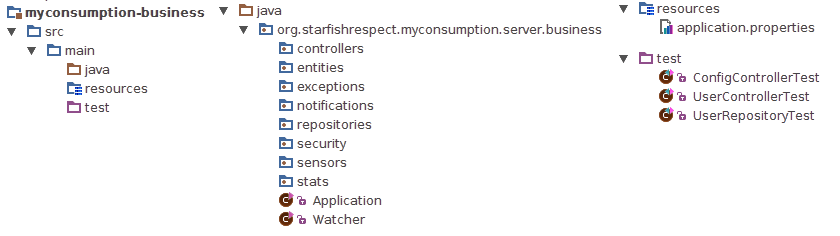
\includegraphics[width=1\textwidth]{back_end_struct.png}}
	\caption{Structure of the server.}
	\label{fig:back_end_struct}
\end{figure}

\subsection{Moving from Spring to Spring Boot}
The first server designed by Patrick was built upon \textit{Spring}. Alongside its other features, this open source framework simplifies dependency injections, allows the deployment of web applications (like RESTful web services), and facilitates database access.\\

Sadly, the configuration of the server was extremely time consuming. It took several days to achieve a working configuration on a new machine because some parts weren’t set correctly (XML configuration files weren’t as modular as they should have been, things tended to crash when refactoring the code etc.). Given this, we decided to move the server to a proper configuration. This move was even more necessary because an open source solution such as the one presented in this work has to be easy to deploy.\\

There simply couldn't have been a better choice than \textit{Spring Boot} to tackle this issue. Indeed, \textit{Spring Boot} makes it easy to create stand-alone, production-grade \textit{Spring} based applications that you can “just run” \cite{Springboot:online}. It provides a faster and accessible getting started experience for all \textit{Spring} development. This tool is relatively new, since the project was started on \textit{Github} in 2013. Using \textit{Spring Boot}, we were able to reuse the code of the previous version of the server with a simple configuration.

\subsection{Maven}
\textit{Spring Boot} comes with \textit{Maven}, a build automation tool used primarily for Java projects. It consists of a \texttt{pom.xml} file which lists all the dependencies of the project. For example, the one below imports the web module of \textit{Spring Boot}:

\begin{lstlisting}[breaklines]
	<dependency>
	    <groupId>org.springframework.boot</groupId>
	    <artifactId>spring-boot-starter-web</artifactId>
	</dependency>
\end{lstlisting}

\textit{Maven} has different \emph{lifecycles}. For example, one can easily package its project just by running: \texttt{mvn package}. Besides lifecycles, plugins can be added to \textit{Maven} in order to better tune the configuration. For example, the plugin \texttt{spring-boot} simplifies the way the server is handled.

\section{RESTful services}
The Representational State Transfer (REST) is a software architecture style, consisting of guidelines and best practices for creating scalable web services \cite{REST:online}. It is a means of expressing specific entities in a system via URL path elements. It minimizes the coupling between client and server components in a distributed application; one of the goals we wanted to achieve.

\subsection{Web server architecture}
The web module of the server is made up of three main packages:
\begin{itemize}
	\item Entities: each one is an object in its simpler form (e.g. a \texttt{User} or a \texttt{Sensor});
	\item Repositories: each one handles specific access to the database;
	\item Controllers: each one deploys a particular web service.
\end{itemize}

\begin{figure}[htbp]
	\centerline{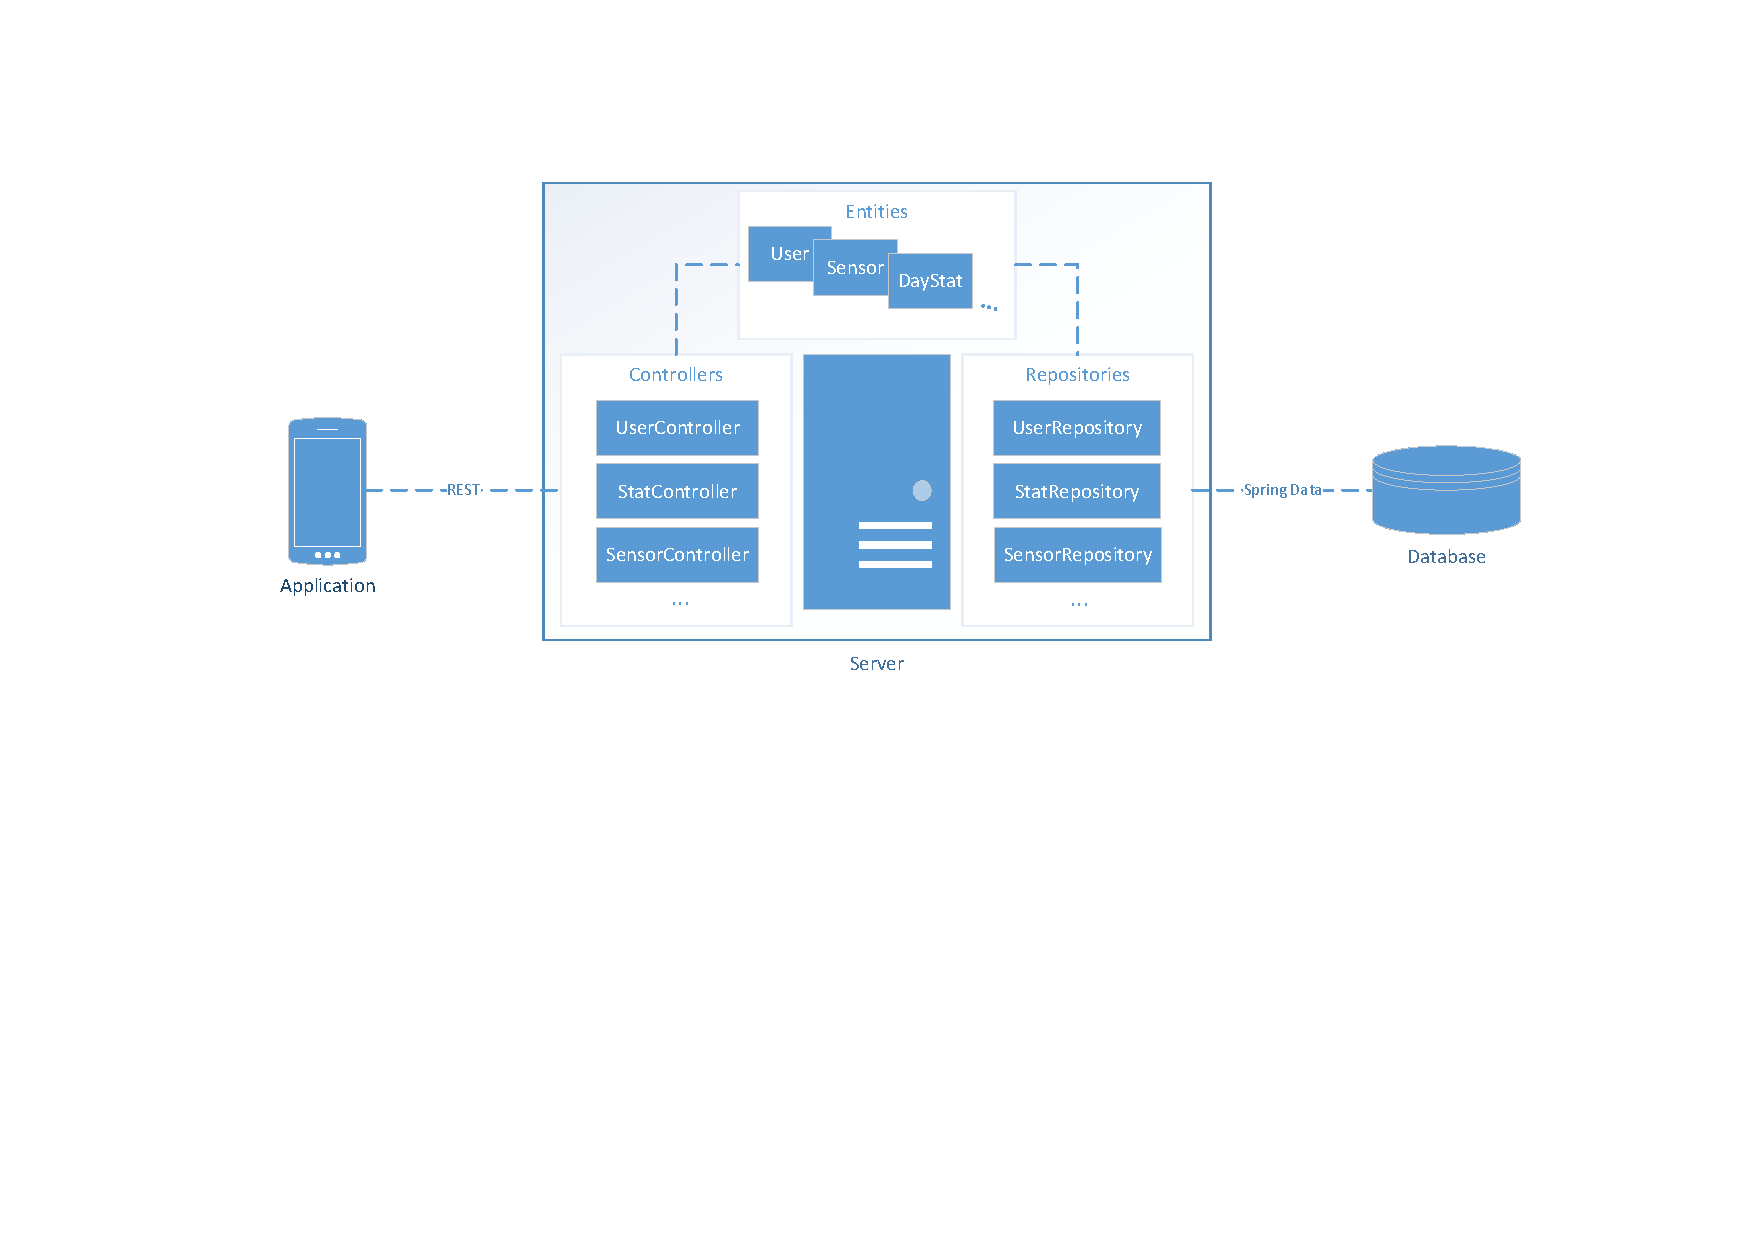
\includegraphics[width=0.9\textwidth]{rep_ent_contr.pdf}}
	\caption{How the server exposes the web services.}
	\label{fig:rep_ent_contr}
\end{figure}

As can be seen in Figure \ref{fig:rep_ent_contr}, each entity is associated with its corresponding controller and repository. For example, the \texttt{User} entity represents a typical user (composed of a name, a password, a list of sensors owned etc.). By using the \texttt{UserRepository}, one can store a given user on the server database. When the application requests information about a particular user, the \texttt{UserController} will try to access the corresponding entity in the database.

\subsection{REST API}
The RESTful API has been built bearing in mind that it should be both friendly to the developer and explorable with a browser address bar. The goal here was to follow some guidelines to make it intuitive, simple and consistent. One of the key principles of REST involves separating the API into logical resources \cite{Sahni:online}. Our resources are: 
\begin{itemize}
	\item Users;
	\item Sensors;
	\item Statistics;
	\item Notifications; 
	\item Configurations.
\end{itemize}

Each resource is represented by a controller. \textit{Spring Boot} controllers are considerably easier to implement than \textit{Spring} ones. All of the code of this section has been updated from \textit{Spring} to \textit{Spring Boot}. Below, Listing \ref{lst:rest_controller} illustrates how to implement such a controller. The latter will return an array of JSON objects representing each sensor. It is accessible at \url{http://myconsumption.s23y.com/sensors}.\\

\begin{listing}[!h]
	\centering
	\begin{tabular}{c}
		\begin{lstlisting}[language=Java]
@RestController
@RequestMapping("/sensors")
public class SensorController {
    @Autowired
    private SensorRepository mSensorRepository;

    @RequestMapping(method = RequestMethod.GET)
    public List<SensorDTO> getAllSensors() {
        return mSensorRepository.getAllSensors();
    }
}
		\end{lstlisting}
	\end{tabular}	
	\caption{Example of a REST controller.}
	\label{lst:rest_controller}
\end{listing}

In the snippet of code Listing \ref{lst:rest_controller}, a lot of annotations are used to tell \textit{Spring Boot} the role of every element. For example:
\begin{itemize}
	\item \texttt{@RestController}: tells that this class is a controller;
	\item \texttt{@RequestMapping("...")}: defines the path to access this resource;
	\item \texttt{@Autowired}: on a property, this annotation allows us to get rid of the setter methods (\textit{Spring} assigns those properties with the passed values or references).
\end{itemize}

The code above was simplified for readability (primarily, security related elements were hidden). Of note is that critical resources of the RESTful service are protected with a layer of security. The user needs to be authenticated to access a resource and (s)he cannot access content that (s)he does not own. This will be discussed in a following section about security.\\

Parameters and other types of request are also supported by \textit{Spring Boot}. The complete description of the API of the RESTful web services is available in the Appendix.

\section{Java API}
Since the application and the server access the same objects between JSON exchanges, a Java API is  provided. It gathers several classes that are common to both of them (see the UML diagram in Figure \ref{fig:dto}). The API is imported to the server and in the application using the dependency injection mechanism. For example, with \textit{Maven}, simply add:
\begin{lstlisting}[breaklines]
	<dependency>
		<groupId>org.starfishrespect.myconsumption</groupId>
		<artifactId>my-consumption-api</artifactId>
		<version>1.0.0-SNAPSHOT</version>
	</dependency>
\end{lstlisting}

\begin{figure}[htbp]
	\centerline{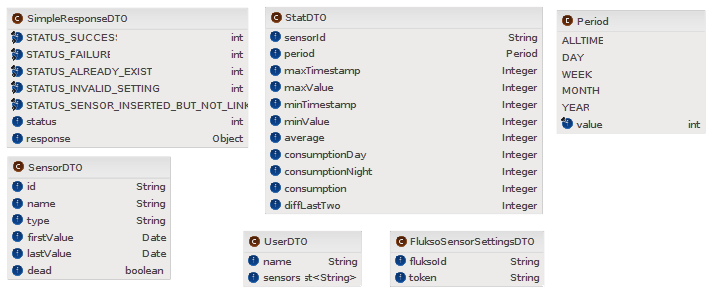
\includegraphics[width=0.95\textwidth]{dto.png}}
	\caption{UML diagram of \textit{MyConsumption} API.}
	\label{fig:dto}
\end{figure}

\section{Retrieve and distribute pricing information}
In the project description, the back end was made responsible for retrieving and distributing pricing information. To retrieve the prices, one idea was to use a public API. Sadly, we were unable to find one. Moreover, it would be quite complex to design the application at an international level because we would have to find pricing information in every country and implement an automatic retrieval on our server for each.\\

We also investigated the possibility of retrieving this information from a website such as a price simulator. Again, this approach would not have been sufficiently scalable and reliable as no generic tool could be found to access the data. \\

We ultimately decided that it was not relevant to investigate or focus further on this retrieval. A workaround was then considered. We defined two values on the server side \cite{levver:online}:
\begin{itemize}	
	\item The peak price:  0.07\euro/kWh;
	\item The off-peak price: 0.0525\euro/kWh.
\end{itemize}

Moreover, a value to convert a kWh to its \(CO_2\) equivalent (in kg) is also given. It is based on an average over the values found in a study \cite{bluesky:online} that compares different energy providers which gave us the value of 0.48 kg of \(CO_2\) per kWh.\\
			
As far as implementation is concerned, a REST service is defined by a controller to give access to the three default values (peak price, off-peak price, and \(CO_2\) conversion).

\section{Managing different users}
A simple user management system was integrated with the server. A \texttt{User} is composed of a name, a password (hashed on the application side, it is never sent in plain text over the network), a list of sensors owned by him/her and a registration ID (an ID associated to the user and the device used with the notification system\footnote{This will be discussed in a following section dedicated to notifications.}).\\

The \texttt{UserController} is responsible for creating, deleting and modifying users. Modification includes the addition or deletion of a sensor owned. Users can only access their own resources and they need to be authenticated. This is discussed in the security section of this work.

\section{The Watcher}
The \texttt{Watcher} is a task whose purpose is to retrieve data from sensors, compute statistics, and send notifications. It is triggered periodically and it consists of a \texttt{Retriever}, a \texttt{StatisticsUpdater} and a \texttt{Notifier}.

\subsection{Retriever}
\emph{Note}: this part comes from the previous version of the server. \\

The goal of the retriever is to collect data from a sensor manufacturer API and store this information in our database. As shown in Listing \ref{lst:sensorretriever}, two methods are used: \texttt{getAllData()} and \texttt{getDataSince()}.

\begin{listing}[!h]
	\centering
	\begin{tabular}{c}
		\begin{lstlisting}[language=Java]
public interface SensorRetriever {
	public abstract SensorData getAllData() throws RetrieveException;
	public abstract SensorData getDataSince(Date startTime) throws RetrieveException;
	public abstract SensorData getData(Date startTime, Date endTime) throws RetrieveException;
}
		\end{lstlisting}
	\end{tabular}
	\caption{The SensorRetriever interface.}
	\label{lst:sensorretriever}
\end{listing}

\subsubsection{A note about modularity}
At the time of writing, only one kind of sensor is supported by the server (\textit{Flukso} sensors). Nevertheless, the design of the retriever allows the simple addition of new types of sensors. Indeed, the retrieval is based on several Java interfaces and generic structures (see Figure \ref{fig:flukso_struct}). If we can match a manufacturer’s API with our interfaces and structures, then we can easily extend the compatibility of the server with this new type of sensor. Thanks to this technique, only the retriever needs to be adapted. The main parts of the server and the mobile application need no change at all.

\begin{figure}[htbp]
	\centerline{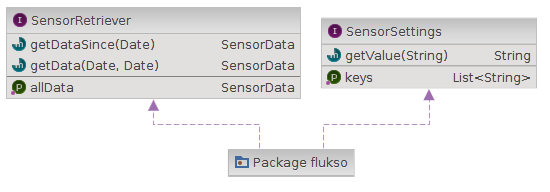
\includegraphics[width=0.7\textwidth]{flukso_struct.png}}
	\caption{The \textit{Flukso}-dependent code implements two interfaces.}
	\label{fig:flukso_struct}
\end{figure}

\subsection{Statistics updater}
The \texttt{StatisticsUpdater} is a key element of the server because many features of the application are based on it. In particular, as described in the design part of this work, we wanted the user to be able to: 

\begin{itemize}
	\item Get an analysis of their own consumption based on statistics;
	\item See their savings between periods;
	\item Compare their consumption to a given consumer profile;
	\item Be notified in case of abnormal consumption. 
\end{itemize}

To address these four features, we defined five periods: a \emph{day}; a \emph{week}; a \emph{month}; a \emph{year}; and \emph{all time}. For each period, we associated a statistical item. We defined:

\begin{itemize}
	\item The consumption over the period (kWh);
	\item The difference between the consumption over this period and the last one (kWh);
	\item The average consumption (W);
	\item The maximum and minimum values (W);
	\item The consumption during high peaks (over the day (kWh)) and off-peaks (over the night (kWh)).
\end{itemize}

This section explains how these items are computed.

\subsubsection{First approach}
The first approach described here came from a significant mistake we made. Indeed, we initially designed the \texttt{StatisticsUpdater} based on a wrong assumption about the overall system. \\

The smart meter API of \textit{Flukso} is designed to return pairs of two values. The first one is the consumption (in Watts) and the second one is the corresponding timestamp. But the tricky thing is that the difference between those timestamps is not constant. Here is what the \textit{Flukso} API returns:
\begin{itemize}
	\item A pair of values every minute for the last 24 hours;
	\item A pair of values every 15 minutes for the last 7 days;
	\item A pair of values every day for the last year;
	\item A pair of values every week for older values.
\end{itemize}

To compute statistics, it is helpful to have a good understanding of the different periods. At the beginning of this work, therein lay our weakness: we designed and implemented the computation of the statistics by mixing values associated with different periods. Of course, the results achieved did not reflect the reality.

\begin{figure}[htbp]
	\centerline{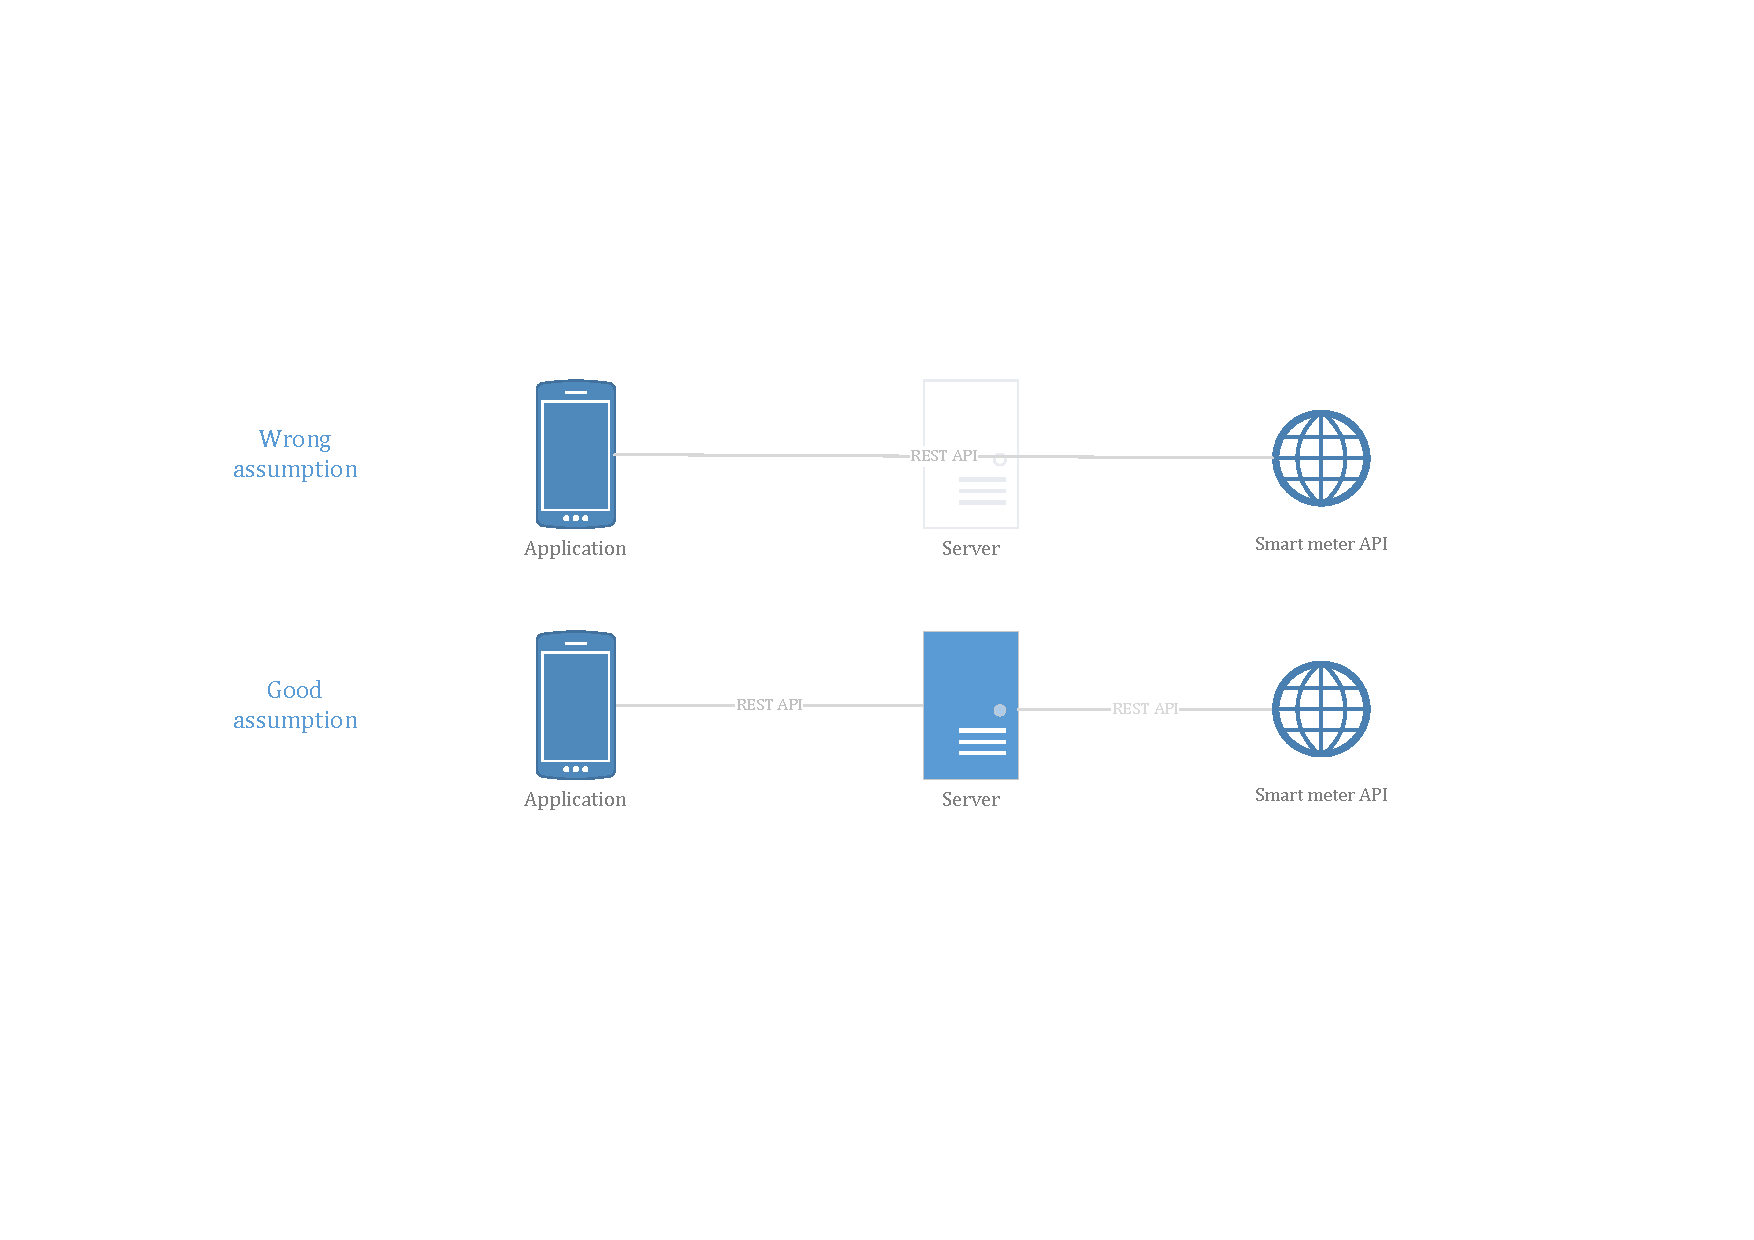
\includegraphics[width=0.9\textwidth]{assumption.pdf}}
	\caption{Misunderstanding of the role of our server.}
	\label{fig:assumption}
\end{figure}

\subsubsection{A second approach}
The crux of the matter is that we were misunderstanding the role of our server (see Figure \ref{fig:assumption}). Indeed, the first approach was designed with the \textit{Flukso} API in mind. This was incorrect because our application has nothing to do with the API of a specific smart meter provider. \\

The only values we should have taken into account were those present in the database of our server. As the server is always on, we chose to keep pairs of values with a difference in timestamp of one minute. This is a far better assumption:  values are no longer mixed and we were able design the computation of the statistics with our server API in mind. This approach also simplified the implementation.

\paragraph{Day by day}
We wanted to compute statistical items over five periods: a day; a week; a month; a year; and all time. We chose to keep a \texttt{DayStat} object in our database. It represents the smaller period (see Figure \ref{fig:daystat}). Every day, we compute a new \texttt{DayStat} with the latest pairs of values retrieved. Other periods are built by adding \texttt{DayStat} objects. For example, a week is simply composed of seven \texttt{DayStats} objects.

\begin{figure}[htbp]
	\centerline{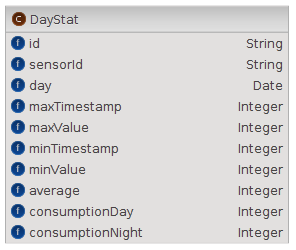
\includegraphics[width=0.35\textwidth]{daystat.png}}
	\caption{A \texttt{DayStat} object.}
	\label{fig:daystat}
\end{figure}

We have values of consumption, measured in Watts. As a power unit, this value describes how much is being used at a given timestamp. The average consumption (W) is simply the average of the values of the day. The maximum and minimum values (W) are likewise intuitive in their formulation. \\

To compute the other values, we needed to convert them in an energy unit (Wh per day). For example, to compute the consumption over the period we started by summing each pair of values. As this value corresponds to Watts taken every 60 seconds, summing these values does not mean much. We need an energy (Wh) which is the total amount of electricity used over a period of time. For a day, this means we had to divide by 60 (the numbers of values taken in one hour). The same process was applied to the consumption during high peaks (over the day (kWh)) and off-peaks (over the night (kWh)).

\paragraph{A note about modularity}
A noteworthy point is that, thanks to the Data Transfer Object (DTO) model and the Java API we provided, the implementation behind every part of the server (and thus the statistics) remains completely independent of the mobile application. We simply have to update the server and match the Java API, and the client does not need to be modified.

\section{Database}
This section describes one of the goals of the back end: ensure synchronization, distribution and backup of energy consumption data.\\

In the design section of this work, we explained the choice of \textit{MongoDb}. It should not be forgotten that this database is not structured around the traditional table-based relational model. Instead, JSON-like documents with dynamic schemas are used. These documents have the advantage of making the integration of data in certain types of applications easier and faster. \\

To communicate with the database, the \textit{Spring Data Framework} was used. It provides a set of \emph{template classes} which are used as a flexible abstraction for working with the data access framework \cite{springdata:online}. We used \textit{Spring Data MongoDb}, which focuses on storing data in \textit{MongoDb}. It inherits functionality from the \textit{Spring Data Commons Project}. With such a framework, we do not have to write any \textit{MongoDb} queries because they are written for us.\\

We defined several entities that are stored in the database. They are described in the UML diagram in Figure \ref{fig:entities}. For example, a \texttt{User} has an ID, a name, a password, a list of sensors and a register ID\footnote{The register ID is used for the \textit{Android} notification system.}. This entity is stored in \textit{MongoDb} with the help of a repository.

\begin{figure}[htbp]
	\centerline{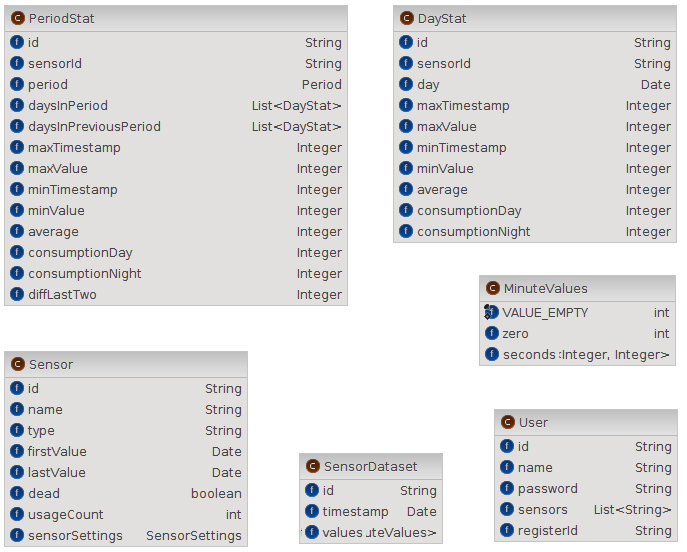
\includegraphics[width=0.9\textwidth]{entities.png}}
	\caption{Entities stored in \textit{MongoDb}.}
	\label{fig:entities}
\end{figure}

\subsection{Moving to Spring Boot}
To explain how entities are stored, it is important to describe some work carried out when we updated the server to \textit{Spring Boot}.\\

The old version of the server was running \textit{Spring} (not to be confused with \textit{Spring Boot}, which simplifies the overall configuration). With \textit{Spring}, specific \textit{MongoDb} operations were used. While this approach enables the programmer to do exactly what (s)he wants, it is prone to errors and needing more code to be written. For example, to access an entity, we would first have to check if it exists before accessing it. Moving to \textit{Spring Boot}  made things even simpler.

\subsubsection{Repository interface}
\textit{Spring Boot} works with repositories. It is an interface that, \emph{out-of-the-box}, comes with many operations, including standard CRUD operations (Create-Read-Update-Delete). The idea is to define queries by simply declaring their method signature. Each repository we created extends some kind of CRUD repository. The latter provides operations to:
\begin{enumerate}
	\item Save the given entity;
	\item Return the entity identified by the given ID;
	\item Return all entities;
	\item Return the number of entities;
	\item Delete the given entity;
	\item Return whether an entity with the given ID exists.
\end{enumerate}

For example, the \texttt{DayStatRepository} is composed of two functions: one to find a sensor by its ID, and another to find a sensor by its ID and date. Here is the code related to this repository:

\begin{listing}[!h]
	\centering
	\begin{tabular}{c}
		\begin{lstlisting}[language=Java]
public interface DayStatRepository extends MongoRepository<DayStat, String> {
    List<DayStat> findBySensorId(String sensorId);
    List<DayStat> findBySensorIdAndDay(String sensorId, Date day);
}
		\end{lstlisting}
	\end{tabular}
	\caption{The DayStatRepository interface.}
	\label{lst:sensorretriever}
\end{listing}

It is indeed fairly simple. Following this, it is only necessary to \texttt{@Autowired} a \texttt{DayStatRepository} where it is needed. After these steps, the two operations above, as well as the basic CRUD operations, are made available.

\subsubsection{CustomRepository}
In the old version of the server, three entities were available: sensor; user; and value. Many operations were already implemented, and we did not want to implement everything again from scratch. A simple solution was to use a \texttt{Custom-} \verb!Repository! interface with a custom implementation. The process to use this scheme is described below:\\

\noindent
1. Define an interface for our custom code:
\begin{lstlisting}[language=Java]
interface CustomUserRepository {
  List<User> yourCustomMethod();
}
\end{lstlisting}


\noindent
2. Add an implementation for this class and follow the naming convention to make sure we can find the class.
\begin{lstlisting}[language=Java]
class UserRepositoryImpl implements CustomerUserRepository {
  private final MongoOperations operations;

  @Autowired
  public UserRepositoryImpl(MongoOperations operations) {
    Assert.notNull(operations, "MongoOperations must not be null!");
    this.operations = operations;
  }

  public List<User> yourCustomMethod() {
    // custom implementation here
  }
}
\end{lstlisting}

\noindent
3. By setting our base repository interface to extend the custom one, the system will automatically use the custom implementation:
\begin{lstlisting}[language=Java]
interface UserRepository extends CrudRepository<User, Long>, CustomUserRepository {}
\end{lstlisting}

In this way we gave ourselves the choice to extend our initial work with the simple configuration of \textit{Spring Boot} and to reuse the existing code in the custom repository implementation (the code from the previous version of the server remains). 

\section{Notify users of abnormal consumption events}
In the design section we discussed the need for an alert system. For example, if the consumption starts to increase in an abnormal way, the mobile application should draw the user’s attention to this fact. \\

The solution we found is called \emph{push notifications}. These are handled via the \href{https://developer.android.com/google/gcm/index.html}{\textit{Google Cloud Messaging}} for \textit{Android}. This service allows data to be sent from our server to all the users' \textit{Android}-powered device. It handles all aspects of queuing of messages and delivery to the target \textit{Android} application. This section explains its implementation in \textit{MyConsumption}.

\subsection{Push notifications: the workflow}
Three actors are involved here: the mobile application; our server; and \textit{Google Cloud Messaging} (GCM). The interactions between the three are described in Figure \ref{fig:notifs}. The workflow is made up of the following steps:

\begin{enumerate}
	\item The \textit{Android} device sends a \texttt{SENDER\_ID} to GCM server for registration;
	\item After successful registration, the GCM server returns a \texttt{REGISTRATION\_ID} to the mobile device;
	\item The mobile device sends this \texttt{REGISTRATION\_ID} to our server;
	\item Our server stores the \texttt{REGISTRATION\_ID} in its database and associates it with the current user of the application;
	\item When our server needs to send a notification to a given user, it sends a request to GCM with the associated \texttt{REGISTRATION\_ID} and message;
	\item GCM sends the push notification to \textit{Android} devices.
\end{enumerate}

\begin{figure}[htbp]
	\centerline{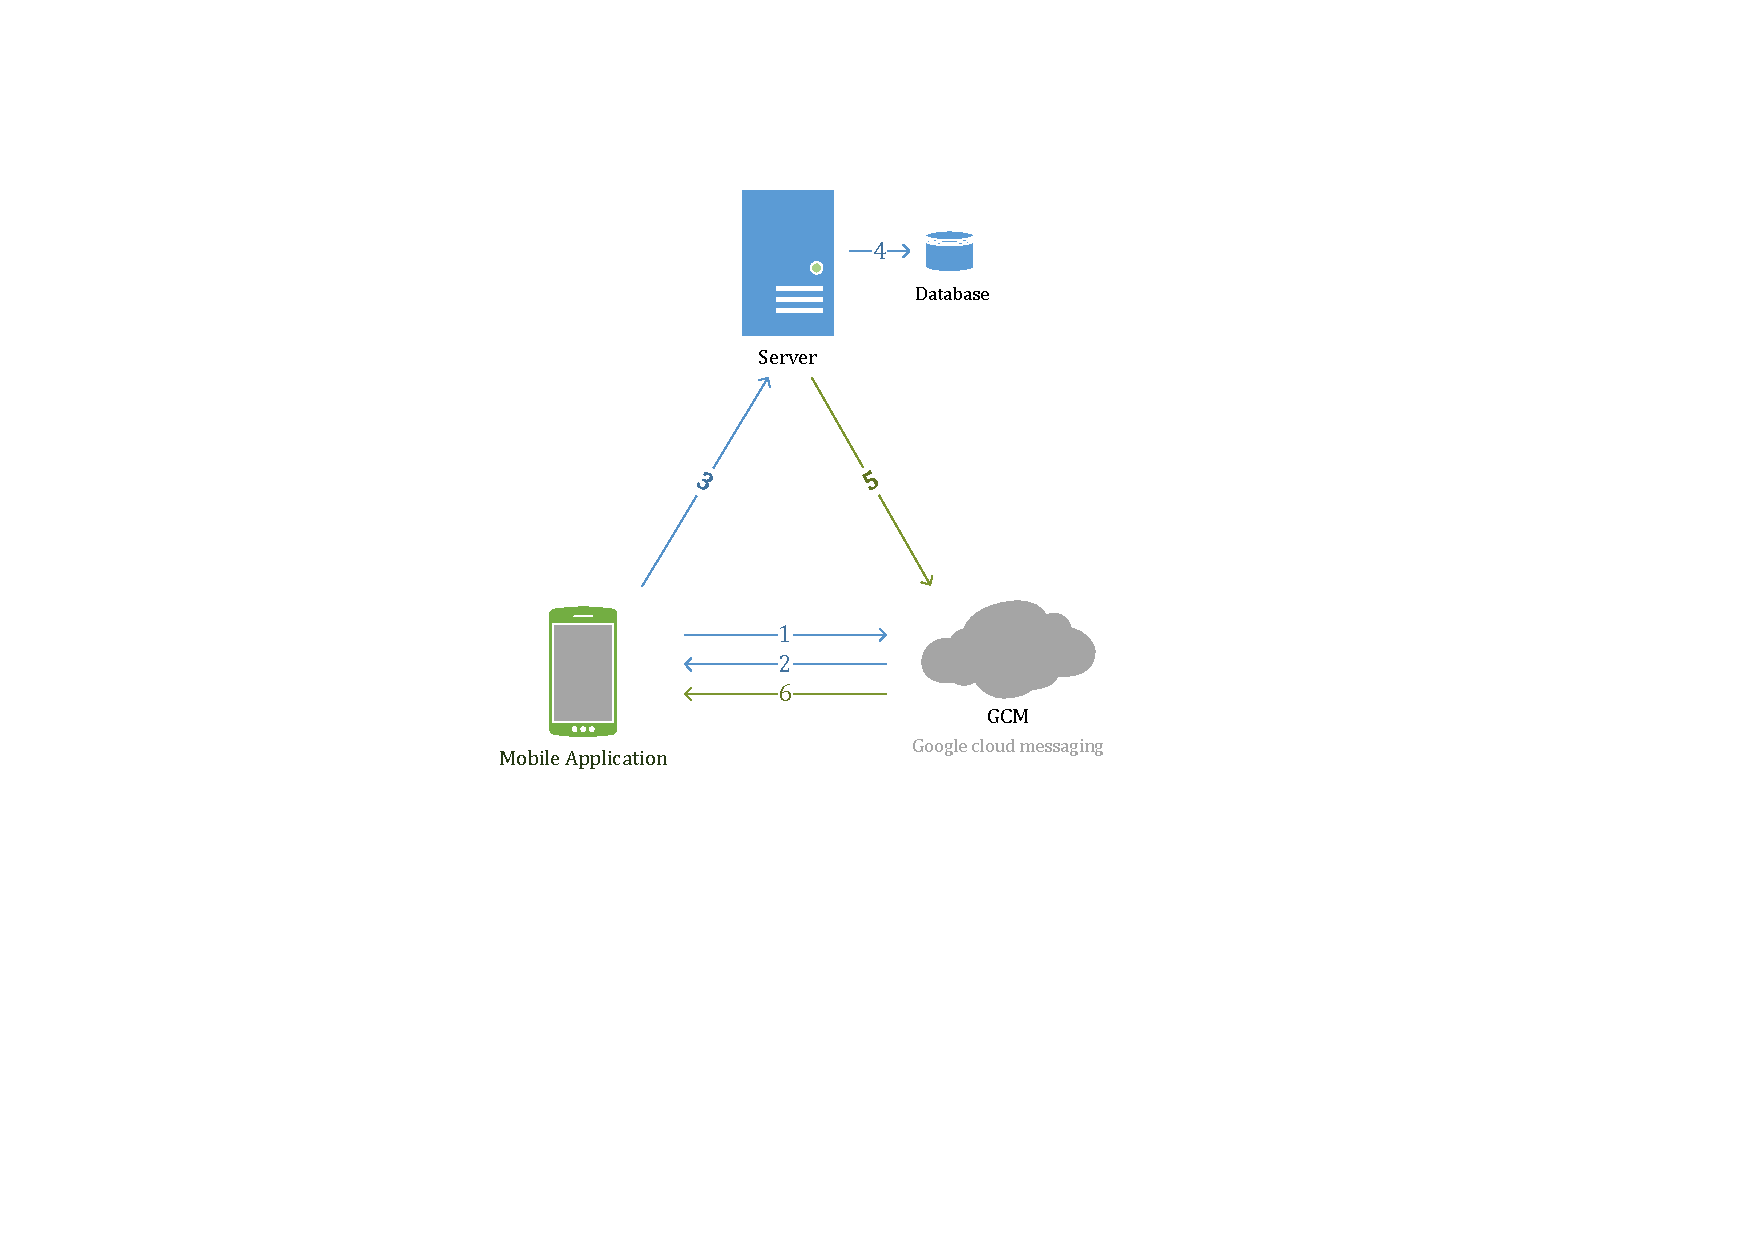
\includegraphics[width=0.6\textwidth]{notifs.pdf}}
	\caption{Notifications workflow.}
	\label{fig:notifs}
\end{figure}

\subsection{When to send a notification}
We first based the sending of notifications on a simple scheme: every day the system told the user if (s)he was consuming more or less than the previous day. This was fine for testing purposes, but in a real environment, we do not want such intrusive notifications. \\

A more appropriate approach was outlined. It involves a threshold and a comparison between the user’s daily consumption and their weekly consumption. Every day, the server checks: 

\[((dayconsumption \times 7) - weekconsumption) > threshold\]

If it is true, then a notification is triggered. The default value of the threshold is 15\%.

\subsection{Server implementation}
\subsubsection{Mobile device registration}
We implemented a controller to allow a mobile user to register for the notification system. A POST request at \texttt{http://myconsumption.s23y.com/notifs/ \{\textit{name}\}/id/\{\textit{regsterId}\}} sets the \texttt{REGISTRATION\_ID} to a given user.
\subsubsection{Send a notification}
Two classes are involved in this process, as outlined below.\\ 

The first class, \texttt{NotificationMessage}, represents a notification message (see Figure \ref{fig:notif_message}). It is composed of different parameters that are described in the GCM server reference. For example, the \texttt{collapseKey} identifies a group of messages that can be collapsed, so that only the last message gets sent when delivery can be resumed. We have used the sensor ID as a \texttt{collapseKey} to avoid pushing multiple notifications for the same sensor.\\

The second class, \texttt{NotificationSender}, builds the request to send to the GCM server. This class is adapted from a Google repository on \textit{Github}. The POST request is sent to https//android.googleapis.com/gcm/send. It is composed of an authorization header with the API Key of \textit{MyConsumption}\footnote{This public API key comes from the Google API project: \url{https://cloud.google.com/console}. It is used as the GCM \texttt{SENDER\_ID}.}. The HTTP body is also described in the GCM server reference.

\begin{figure}[htbp]
	\centerline{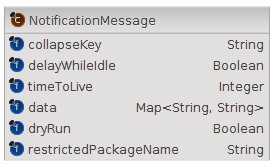
\includegraphics[width=0.4\textwidth]{notif_message.png}}
	\caption{Representation of a notification message.}
	\label{fig:notif_message}
\end{figure}

\section{Security}
In the design section of this work, different security mechanisms were detailed. At the end of the discussion, basic authentication over HTTPS was chosen because it meets the desired level of security while keeping the configuration and the implementation simple. The latter is described in this section.

\subsection{Authentication}
To add the desired level of security, we used the \texttt{spring-security} dependency. The two classes involved in the configuration are outlined below. Each one extends a default class of \textit{Spring Security} to tune its configuration.\\ 

In \texttt{AuthConfig}, we simply bind our \texttt{User} entity to the one used in \textit{Spring Security} (\texttt{UserDetails}). Thanks to this, users are now recognized by the authentication system of the server. \\

In \texttt{WebSecurityConfig}, we defined some specific policies. Indeed, when creating a new user on the application side, we are not yet able to authenticate. Accordingly, the service to create a user is accessible through anonymous authentication. Another interesting thing to note here is that this approach forces the server to have a stateless behavior, as  advised in the design section.\\

The rest of the work is done by \textit{Spring Security}. Each request requires an \texttt{Authorization: Basic} header followed by the Base64 encoded username: password pair. Moreover, we will see in the next chapter that the password is not sent as plain text over the network.

\subsection{Authorization}
Since we mapped our \texttt{User} implementation with \textit{Spring Security}, it is possible to retrieve the identity of a specific user when (s)he tries to access a resource. This is done using a particular class of \textit{Spring Security}: \texttt{Principal}. Thanks to this, it is possible to check whether the user has the right to access the desired content. In general, the simple check detailed below is enough.
\begin{listing}[!h]
	\centering
	\begin{tabular}{c}
		\begin{lstlisting}[language=java]        
if (!(principal.getName().equals(name)))
    return new SimpleResponseDTO(false, "you are not allowed to modify this user");
		\end{lstlisting}   
	\end{tabular}
	\caption{Check if a user can access a resource.}
	\label{lst:authorization}
\end{listing}		         

\subsection{Storing the credentials}
As the password is hashed on the client side, it is stored as it is received on the server database. The one way hash provide a first layer of security. However, to prevent attacks with rainbow tables, it could be better to use a randomly generated salt with the hash.

\subsubsection{Setting up HTTPS for Spring Boot}
HTTP protocol vulnerabilities, man-in-the-middle attacks, replay attacks and unencrypted exchanges can be avoided by using HTTPS. With \textit{Spring Boot}, the configuration is simple: in the \texttt{application.properties} file, SSL is supported by adding the following information about the certificate.\\

\begin{listing}[!h]
	\centering
	\begin{tabular}{c}
		\begin{lstlisting}[breaklines]
server.port = 8443
server.ssl.key-store = classpath:keystore.jks
server.ssl.key-store-password = secret
server.ssl.key-password = another-secret
		\end{lstlisting}
	\end{tabular}
	\caption{Setting up HTTPS for \textit{Spring Boot}.}
	\label{lst:https}
\end{listing}

That is all it takes to set up HTTPS. However, even if one can generate a self-signed certificate for testing purposes, a real one will be needed for a release. Sadly, the latter needs to be signed by a certified authority. This process is paying and has not been done in the scope of this work.

\chapter{Front end}
The role of the \textit{Android} application is to display data fetched from the server. While implementing the client, we tried to minimize the computational load on its side. In the future, this could help in porting the application to another platform. As far as \textit{Android} is concerned, this application runs on 90\% of the device active on the \textit{Google Play Store}\footnote{On  March 19, 2015.}.\\

This part of the work aims to describe the choices made while implementing the mobile application. First, its structure is detailed. Next, some \textit{Android} related concepts are introduced and described in the case of \textit{MyConsumption}, such as activities, fragments and services. After that, internal communication is addressed. Finally, a section is dedicated to the data management.

\section{Structure of the application}
The  package hierarchy of the front end is illustrated in Figure \ref{fig:front_end_struct}. Under the path \texttt{app/src/main}, two folders and a file are available: 

\begin{itemize}
	\item \texttt{java}: groups the java packages and classes;
	\item \texttt{res}: groups the XML resource files and folders;
	\item \texttt{AndroidManifest.xml}: a file which presents essential information which the system must have before it can run any of the application's code.
\end{itemize}

\begin{figure}[htbp]
	\centerline{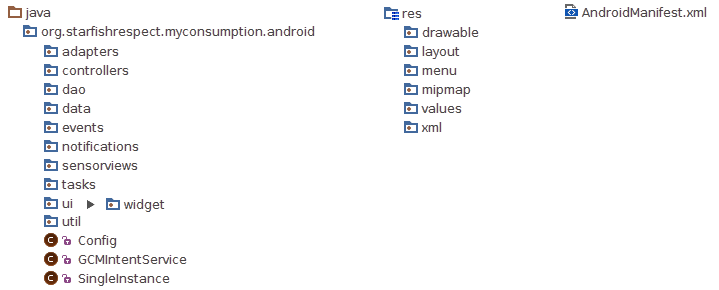
\includegraphics[width=0.95\textwidth]{front_end_struct.png}}
	\caption{Structure of the application.}
	\label{fig:front_end_struct}
\end{figure}


The Model-View-Controller (MVC) architecture is used to design \textit{Android} applications. The idea is that any object in an application must be either a model object, a view object, or a controller object \cite{bignerch:book}.
\begin{itemize}
	\item A \emph{model object} keeps the application’s and data “business logic”. These objects do not have any knowledge of the user interface; they only aim at holding and managing the data. In \textit{Android}, this category generally includes the classes we create, such as a user, a product in a store etc. Together they compose the \emph{model layer}.
	\item \emph{Views objects} are the those which know how to draw themselves on the screen. They also know how to respond to user input. Essentially, the things that can be seen on screen are views. This category mainly consists of widgets that are inflated from an XML layout. Together they form the \emph{view layer}.
	\item \emph{Controller objects} link the view and model objects. They hold the “application logic”. They are designed to respond to events triggered by view objects. They also manage the flow of data to and from model objects and the view layer. In \textit{Android}, a controller is typically a subclass of \texttt{Activity}, \texttt{Fragment} or \texttt{Services}.
\end{itemize}

\section{XML files}
\subsection{Layouts}
A layout describes the visual structure of a graphical user interface, such as the UI for an activity or an application widget. They can be declared in two ways: using an XML file or by instantiating layout elements at runtime. Nevertheless, it is recommended to declare UI in XML because it enables better separation of the application’s presentation from the code that controls its behavior. 
In \textit{MyConsumption}, four types of layouts are defined under the \texttt{res/layout} folder. They describe \texttt{Activities}, \texttt{Fragments}, \texttt{Widgets} and \texttt{items}. They are all declared using XML files.

\subsection{Styles}
We focused on making the mobile application intuitive and visually attractive. In \texttt{styles.xml}, a theme is defined: \texttt{Theme.MyConsumption.Base}. It describes the main colors, the default background, and some high level configurations to be used everywhere in the app. The theme of some widgets, such as the header bar, are also defined here.

\subsection{Resolutions and orientations}
Different resolutions are taken into account through the use of fragments (see section below). Moreover, specific dimensions are defined for three types of screen sizes in the three \texttt{dimens.xml} files:  for \texttt{w820dp}\footnote{\emph{Density-independent pixel} (dp) is a virtual pixel unit used when defining UI layout, to express layout dimensions or position in a density-independent way \cite{screen:online}.}  screens, \texttt{sw600dp} and a default configuration for the others.\\

As far as the screen orientation is concerned, different layouts are provided for the statistics screen and the comparison one. They both have a specific look in portrait and landscape mode. 

\subsection{Other XML files}
Strings, values, arrays, preferences, drawables and menus are also defined in specific XML files, as recommended by the \textit{Android} documentation.

\section{Activities and fragments}
An \emph{activity} is a single, focused thing that the user can do \cite{activity:online}. In brief, it is a window where we can place UI elements. As a user navigates through, out of, and back to the app, the Activity instances transition between different states in their lifecycle (see Figure \ref{fig:lifecycle}).\\

\begin{figure}[htbp]
	\centerline{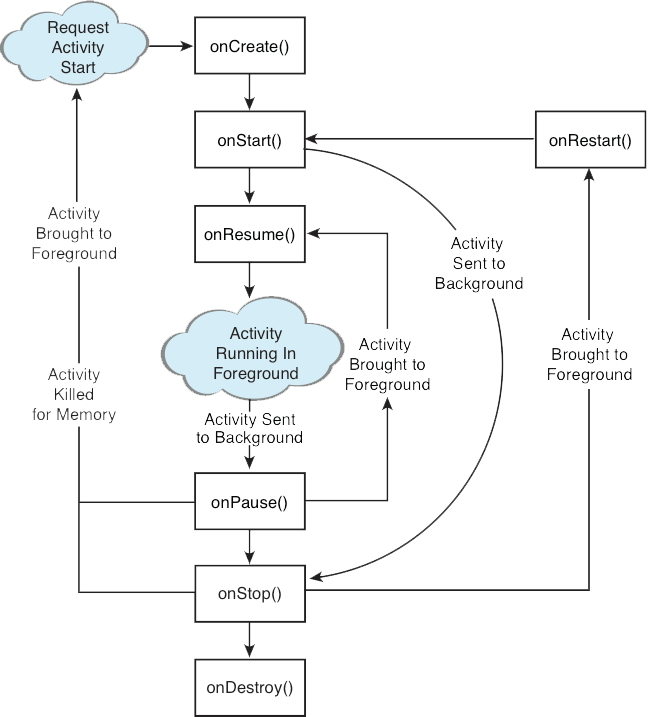
\includegraphics[width=0.65\textwidth]{lifecycle.png}}
	\caption{The lifecycle of an \textit{Android} \textit{Activity} \cite{introandroid:book}.}
	\label{fig:lifecycle}
\end{figure}

A \emph{fragment} is a piece of an application's user interface or behavior that can be placed in an activity \cite{fragment:online}. A key feature of fragments is that they can be used as an application's layout. This allows a better modularization of the code and to easy adjustment of  UI to different screens (tablets, smartphones, TVs etc.). Just as for activities, fragments have their own lifecycle.\\

The design part of this report describes user interfaces, mockups and use cases. Their implementation is described below. The files related to this section are located in the package \texttt{ui}.

\subsection{Login}
The \texttt{LoginActivity} comes from the previous version of the application. The layout has been improved to better match small screen sizes. This activity is displayed on the first launch of the application. Subsequently, user credentials are stored on the device.\\

If the user has no credentials, an option is available to create a new account by entering a name and a password. This is handled by the \texttt{CreateAccountActivity} (which comes also from the previous version of the application).

\subsubsection{A note about security}
In the previous version of the application, the user’s password was only useful on the client side to log in. In the current version, the server is secured, meaning that we need those credentials for authentication purposes. The plaintext password is hashed and stored in the application’s local database with the username. The content of the database can be accessed with root privileges, though the hash provides some degree of protection.

\subsection{Switching screens}
In the design part of this work, a use case describes how the user should switch between screens. A common way to do this on modern \textit{Android} applications is to use a Navigation Drawer (see Figure \ref{fig:nav_drawer}).  This is a panel that displays the main navigation options. It is located on the left edge of the screen and is hidden most of the time. It is revealed when the user swipes from the left edge of the screen, or when (s)he touches the app icon in the header bar.

\begin{figure}[htbp]
	\centerline{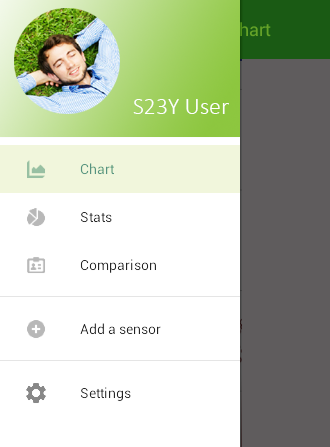
\includegraphics[width=0.32\textwidth]{nav_drawer.png}}
	\caption{The navigation drawer.}
	\label{fig:nav_drawer}
\end{figure}

\begin{figure}[htbp]
	\centerline{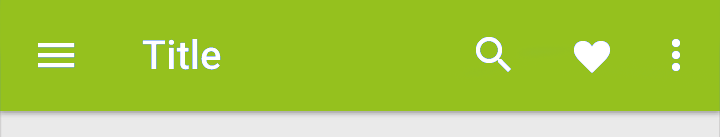
\includegraphics[width=0.4\textwidth]{headerbar.png}}
	\caption{A header bar.}
	\label{fig:headerbar}
\end{figure}

\subsection{BaseActivity}
At the beginning of the project, we had trouble properly managing the activities with the navigation drawer and the header bar (see Figure \ref{fig:headerbar}). Different parts of the code were duplicated and interdependent. At a certain point, it became clear that it was simply not scalable.\\

The design presented below was inspired by one of the most popular \textit{Android} repositories on \textit{Github}: the \href{https://github.com/google/iosched}{Google I/O 2014 \textit{Android} App}. This application has been a great source of inspiration and a reference while building \textit{MyConsumption}. Indeed, it is full of features, built by Google engineers and widely reviewed. As a result, \textit{MyConsumption} has grown in modularity.\\

In short, as illustrated in Figure \ref{fig:base_activity}, every important screen of the application extends the \texttt{BaseActivity}. The latter is an abstract class whose purpose is to regroup the elements that are reused in every Activity. Two important widgets are defined and handled in \texttt{BaseActivity}: the header bar and the navigation drawer. Moreover, common features of the app (such as the reloading option) are also implemented there. Adding a new activity to the navigation drawer is straightforward. Here are the steps in \texttt{BaseActivity}:
\begin{itemize}
	\item Add the title of the new activity to the \texttt{NAVDRAWER\_TITLE\_RES\_ID} array;
	\item Add a corresponding icon to the \texttt{NAVDRAWER\_ICON\_RES\_ID} array;
	\item In the method \texttt{populateNavDrawer}(), add the new item to the list;
	\item Add a case in \texttt{goToNavDrawerItem}() to launch the new activity.
\end{itemize}

\begin{figure}[htbp]
	\centerline{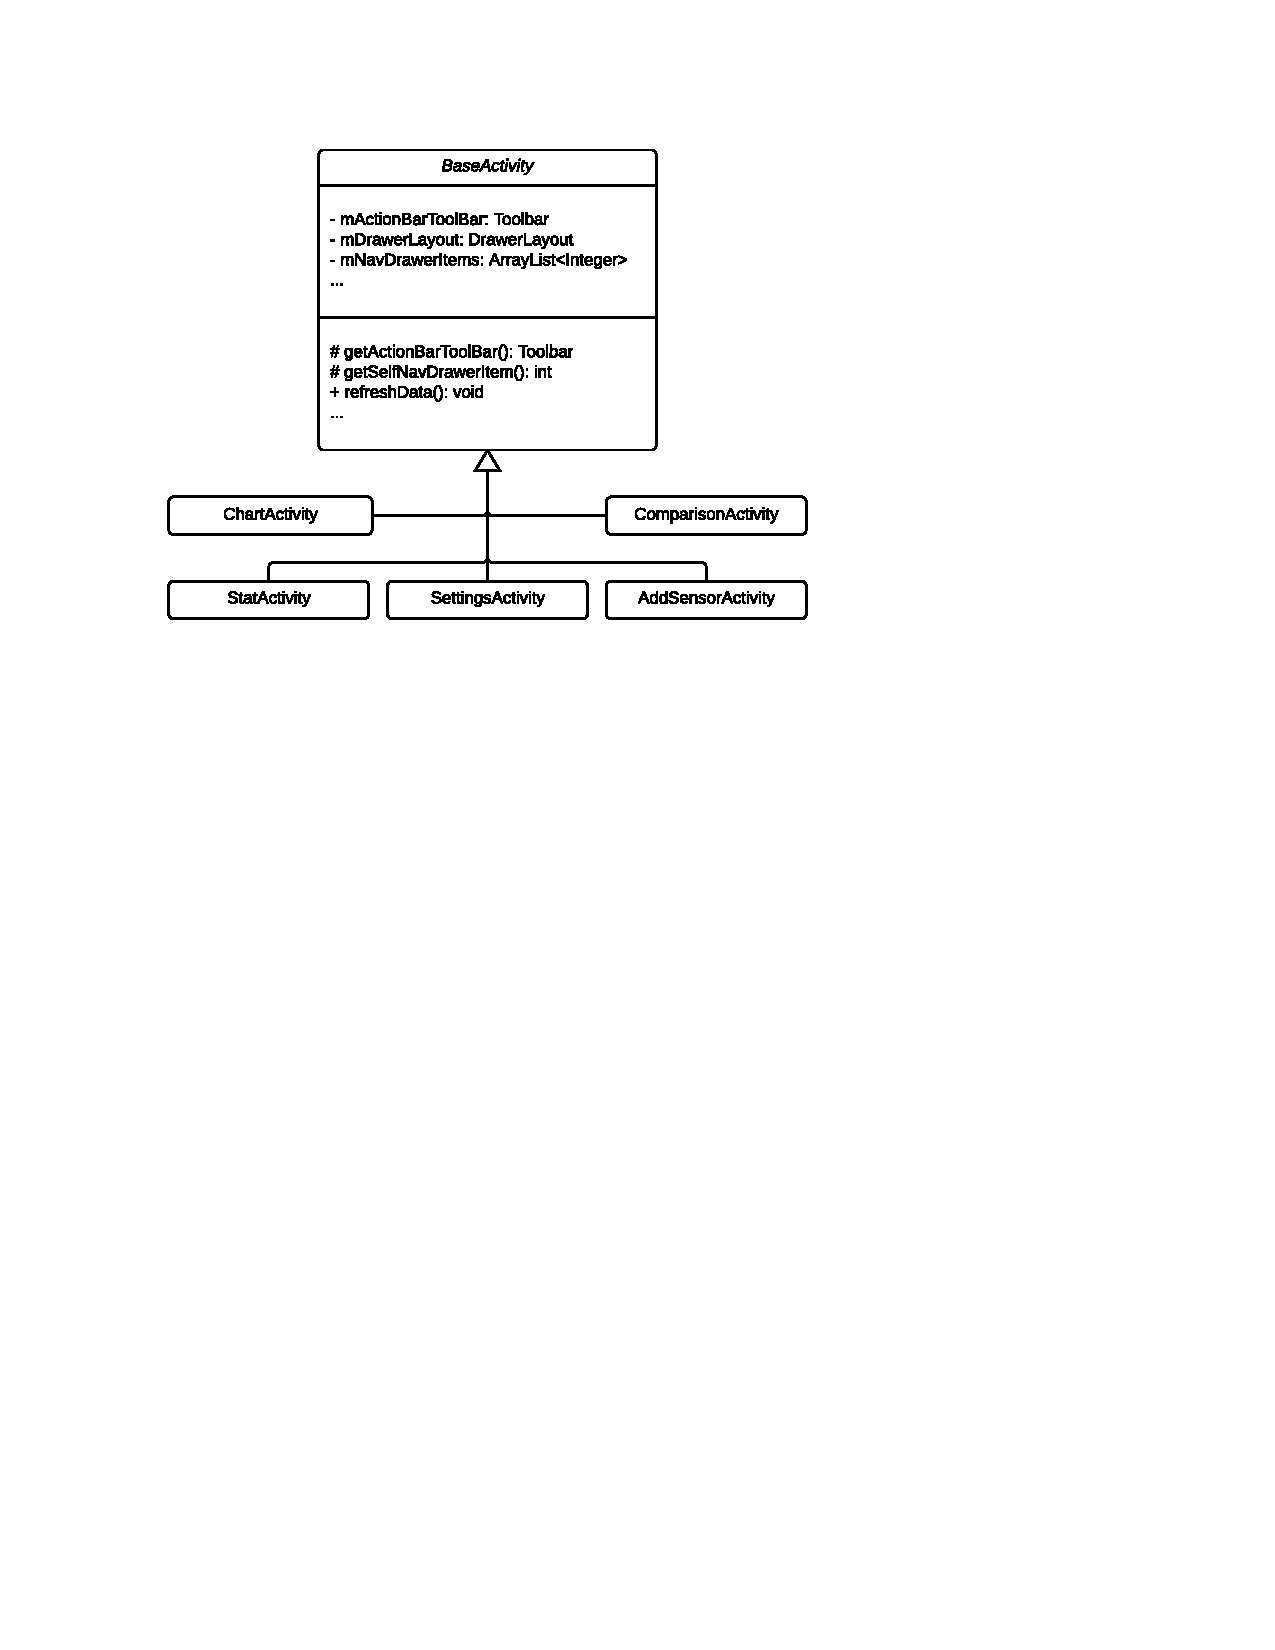
\includegraphics[width=0.6\textwidth]{base_activity.pdf}}
	\caption{The activities that extend \texttt{BaseActivity}.}
	\label{fig:base_activity}
\end{figure}

As a result, the code of a new activity is quite short. The Listing \ref{lst:helloworld_activity} shows the \texttt{HelloWorldActivity} class, which is a template that can be reused when creating a new activity. It is short and, thanks to \texttt{BaseActivity}, it supports \emph{out-of-the-box} the navigation drawer and the header bar with menu items.
\begin{listing}[!h]
	\centering
	\begin{tabular}{c}
		\begin{lstlisting}[language=java]
public class HelloWorldActivity extends BaseActivity {
	@Override
	protected void onCreate(Bundle savedInstanceState) {
		super.onCreate(savedInstanceState);
		setContentView(R.layout.activity_main );
		Toolbar toolbar = getActionBarToolbar();
		toolbar.setTitle("My Consumption - HelloWorld");
		overridePendingTransition (0, 0);
	}

	@Override
	protected int getSelfNavDrawerItem() {
		// set this to have a nav drawer associated with this activity
		return NAVDRAWER_ITEM_HELLO_WORLD;
	}
}
		\end{lstlisting}
	\end{tabular}
	\caption{The \texttt{HelloWorldActivity} which extends \texttt{BaseActivity}.}
	\label{lst:helloworld_activity}
\end{listing}

\subsection{Main screen: ChartActivity}
The \texttt{ChartActivity} is the first screen one can see when opening the application. This Activity was already present in the previous version of the application but it has been integrated with \texttt{BaseActivity} to match the overall design and behavior of \textit{MyConsumption}. \\

The two fragments \texttt{ChartChoiceFragment} and \texttt{CharViewFragment} composes this screen. The first fragment displays the option on the right while the second one contains the chart itself. The chart is built with \textit{Achartengine}, a library under the license Apache 2.0. It handles zooming, scrolling, and selecting data by clicking on them.

\subsection{Graph smoothing}
In the offices of S23Y, the electrical devices are configured such that high peaks appear in the electricity consumption chart (see Figure \ref{fig:chart_high_peaks_removed}). For the user, it is not always relevant to see those peaks. He/she might want to see only the general trend of their consumption on the graph. To  achieve this purpose, a new option was given to the user to allow him/her to smooth the graph. As illustrated in Figure \ref{fig:seekbar}, we used a seek bar which makes it possible to select a value from a range by moving the slider thumb \cite{seek:online}.

\begin{figure}[htbp]
	\centerline{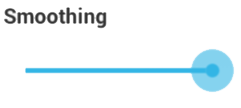
\includegraphics[width=0.28\textwidth]{seekbar.png}}
	\caption{ The seek bar.}
	\label{fig:seekbar}
\end{figure}

The smoothing algorithm behind the inteface is a simple moving average. It creates a series of averages of different subsets of the full data set \cite{movingavverage:online}. The reason for this choice is that the number of points displayed on the screen is relatively low (about 500). Consequently, an algorithm with a complexity of \(O(n)\) is enough for something computed on the client side. Additionally, the formula is quite simple:
\[\bar{x}_n = \bar{x}_{n-1} + \frac{ x_n - x_{n-N} }{N}\]

The result is illustrated in Figure \ref{fig:chart_high_peaks_removed}.

\begin{figure}[htbp]
	\centerline{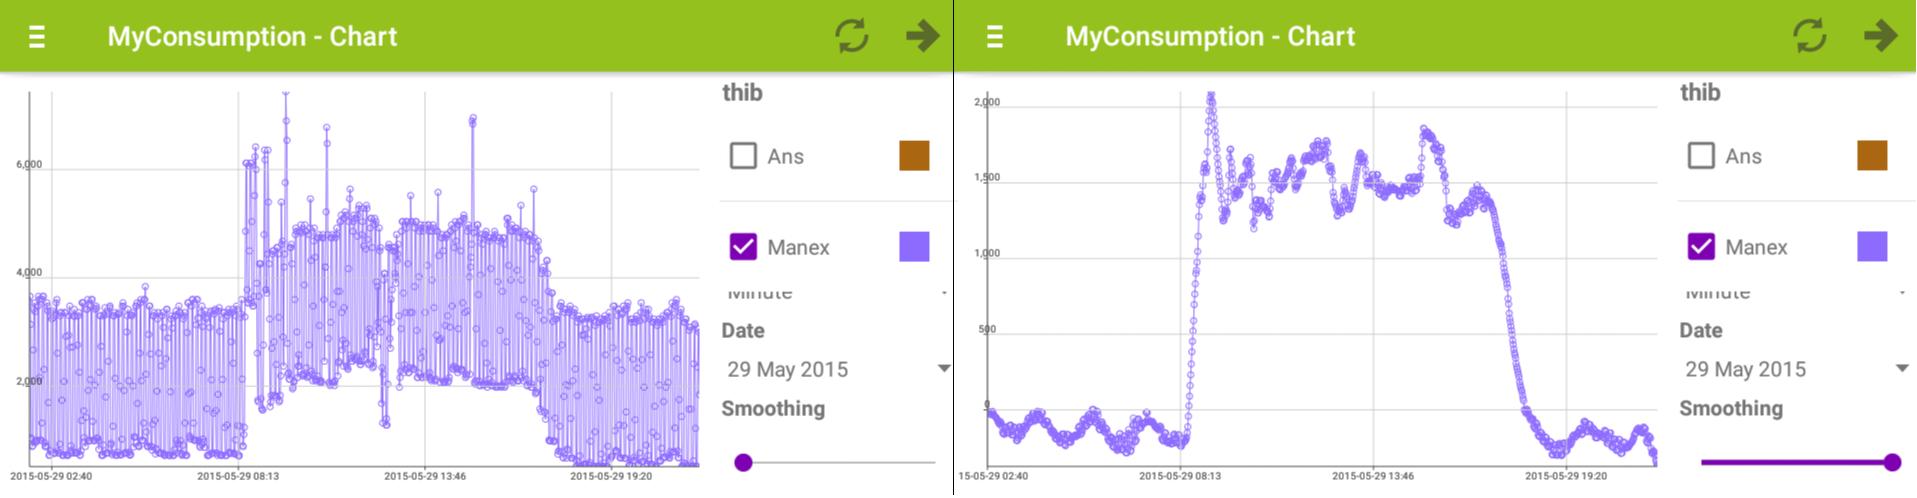
\includegraphics[width=1\textwidth]{chart_high_peaks_removed.png}}
	\caption{Smoothing option (be aware that the y-axis range has changed).}
	\label{fig:chart_high_peaks_removed}
\end{figure}

\subsection{Statistics}
This screen gathers different features described in the design part of this work. The main goal of the \texttt{StatActivity} is to provide an analysis of consumption based on statistics, but it also includes the savings between periods as well as the need to retrieve pricing information from our server.\\

Statistics are computed on the server side; \texttt{StatActivity} is only in charge of displaying them. In order to do so, sliding tabs are used. We chose to include a library for this purpose: \href{https://github.com/astuetz/PagerSlidingTabStrip}{\textit{PagerSlidingTabStrip}} (see Figure \ref{fig:pager}).

\begin{figure}[htbp]
	\centerline{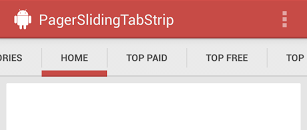
\includegraphics[width=0.4\textwidth]{pager.png}}
	\caption{The pager sliding tab strip.}
	\label{fig:pager}
\end{figure}

In \texttt{StatActivity}, an adapter is used to handle the tabs. Each item of this adapter instantiates a \texttt{SlidingStatFragment} which represents the content of each tab. A factory method is used here to create each instance of the fragment. It is the public static method: \texttt{SlidingStatFragment.newInstance(...)}.\\

The \texttt{SlidingStatFragment} is composed of \texttt{LinearLayouts} to build the UI. The pie chart is created by using a \texttt{PieData} object from the \href{https://github.com/PhilJay/MPAndroidChart}{\textit{MPAndroidChart}} library. The choice of this library was motivated by: the popularity of the library on \textit{Github}; its simplicity; and the large panel of features it offers (which might be useful for future developments).

\subsection{Profile comparison}
The \texttt{ComparisonActivity} allows the user to compare their consumption to a given consumer profile. The profile is defined in the preferences of the application and will be discussed later.\\

The UI of this activity is essentially based on \texttt{LinearLayouts} and a \texttt{BarChart} object from the \textit{MPAndroidChart} library. From an implementation perspective, this Activity is quite similar to \texttt{StatActivity}.

\subsection{Preferences}
The settings of the application are built upon the \href{https://developer.android.com/guide/topics/ui/settings.html}{\textit{Android}'s Preference APIs}. Every setting for the app is represented by a specific subclass of the \texttt{Preference} class of this API. A screenshot of this Activity is given in Figure \ref{fig:settings_land}. \\

As far as \textit{MyConsumption} is concerned, we chose to group the preferences in two categories: user profile and synchronization. Inside the app, the preferences are easily accessible through a class called \texttt{PrefUtils}.

\begin{figure}[htbp]
	\centerline{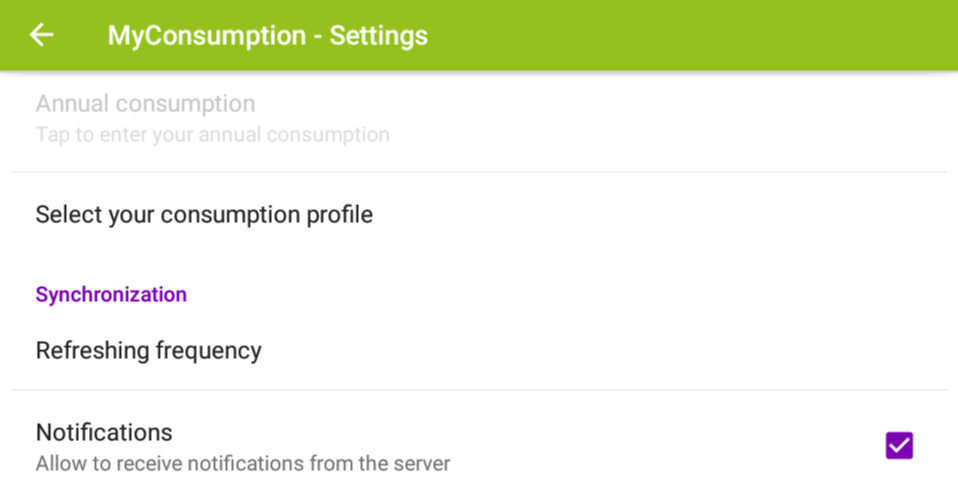
\includegraphics[width=0.65\textwidth]{settings_land.png}}
	\caption{The settings of the application.}
	\label{fig:settings_land}
\end{figure}

\subsubsection{User profile}
As described in the “Profile comparison” section, each user can choose a consumer profile between the three following ones:
\begin{itemize}
	\item Studio / apartment with refrigerator: 600 kWh / year;
	\item Small family using a dishwasher + refrigerator: 1200 kWh / year;
	\item Average family with electric appliances + electric water heater: 3,500 kWh.
\end{itemize}
Those profiles were defined based on the CWAPE\footnote{CWAPE: \textit{Commision Wallonne pour l’Énergie} (\url{http://www.cwape.be/}).} simulator and a paper of the CREG\footnote{CREG: \textit{Commision de régulation de l’électricité et du gaz} (\url{http://www.creg.info/}).} \cite{CWAPE:online, creg:article}.

\subsubsection{Synchronization}
A background task refreshes periodically the data from the server. Its refreshing frequency can be set in the preferences to 5, 10, 15 or 20 minutes. Moreover, the user can choose whether he wants to receive notifications.

\section{Internal communication}
Many elements communicate between each other in an \textit{Android} application. For example, network operations are always performed in a separate thread from the UI\footnote{It is done this way to prevent  a poor user experience due to unpredictable delays in network connections.}. Thus, such an asynchronous task has to communicate the result of its execution with the main thread. This is not the only example: a fragment may want to deliver a particular message to its parent activity; views have to report that they have been modified (e.g. a button clicked); a background task is conducted; etc. This is illustrated in Figure \ref{fig:status_quo}.

\begin{figure}[htbp]
	\centerline{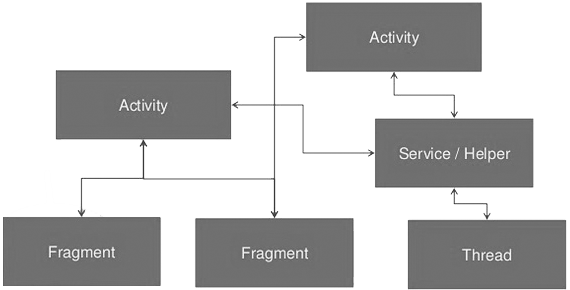
\includegraphics[width=0.6\textwidth]{status_quo.png}}
	\caption{The complexity of internal communications in Android \cite{Eventbusslide:online}.}
	\label{fig:status_quo}
\end{figure}

Of course, there is a way to handle those events in \textit{Android}: by using callbacks.  First, we have to define the callback interface:
\begin{lstlisting}[language=java]
interface MyCallback {
    void callbackCall();
}
\end{lstlisting}
Then, in a worker (e.g. an asynchronous task), we define this callback as a member of the class and we trigger the event at the right place and time:
\begin{lstlisting}[language=java]
class Worker {
   MyCallback callback;

   void onEvent() {
      callback.callbackCall();
   }
}
\end{lstlisting}
Finally, we handle the callback call by implementing the interface:
\begin{lstlisting}[language=java]
class Callback implements MyCallback {
   void callbackCall() {
      // callback code goes here
   }
}
\end{lstlisting}

The process presented above is fine for simple operations. However, as soon as we move away from one of the few well-defined scenarios where \textit{Android} can indeed update its views when background tasks result, things become more complex. As advised in the \textit{Android} documentation, we used child classes of \texttt{AsyncTask} for all background works. These are launched in a different thread of the UI. \\

Nonetheless, the common following scenario is hard to manage. As soon as the activity view is displayed, we start an asynchronous task to load data from the server. At the end of its execution, a natural approach would be to tell the \texttt{AsyncTask} the modification to make on the view. This, however, is not the right way of doing things. Indeed, if the user rotated the device, the view would be destroyed and replaced by a new one. Thus, the \texttt{AsyncTask} would then have a reference pointing to a view which is no longer displayed.

\subsection{An initial approach}
The first solution employed to solve this problem was to use a Singleton which kept pointers to fragments and activities. By assigning tags when creating activities and fragments, we were able to get the references back to them in the Singleton even if they were destroyed by the \textit{Android} system at a given time. Nevertheless, this homemade workaround had some drawbacks: it was hard to maintain and prone to errors.

\subsection{A better solution: the event bus}
The solution we subsequently found comes from a project found on \textit{Github}: the \href{https://github.com/greenrobot/EventBus}{\textit{EventBus}}. This is a publish/subscribe event bus optimized for \textit{Android}, which simplifies the communication between components. It acts like the \emph{Observer} pattern (see Figure \ref{fig:eventbus} and \ref{fig:publish_subscribe}). It is quite simple and it solves the problem of null references.

\begin{figure}[htbp]
	\centerline{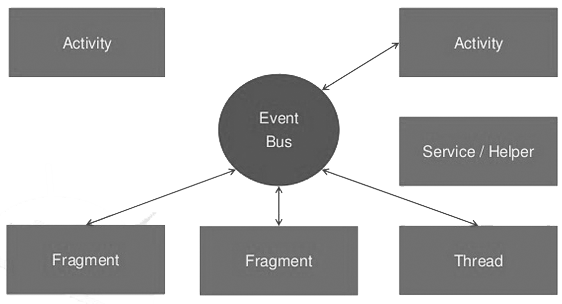
\includegraphics[width=0.6\textwidth]{eventbus.png}}
	\caption{Event bus communication \cite{Eventbusslide:online}.}
	\label{fig:eventbus}
\end{figure}

Firstly, an event must be defined. Luckily, they are simple Java objects which we can design as we please (see Listing \ref{lst:eventbus_sample}).\\

\begin{listing}[!h]
	\centering
	\begin{tabular}{c}
		\begin{lstlisting}[language=java]
public class MessageEvent {
    public final String message;

    public MessageEvent(String message) {
       this.message = message;
    }
}
		\end{lstlisting}
	\end{tabular}
	\caption{An event message for the \textit{EventBus}  \cite{Eventbusslide:online}.}
	\label{lst:eventbus_sample}
\end{listing}

Following this, subscribers (activities, fragments or other components) implement event handling \texttt{onEvent} methods that will be called when an event is received. They also need to register and unregister themselves to the bus (see Figure \ref{fig:publish_subscribe} and Listing \ref{lst:eventbus_reg_unr}).

\begin{figure}[htbp]
	\centerline{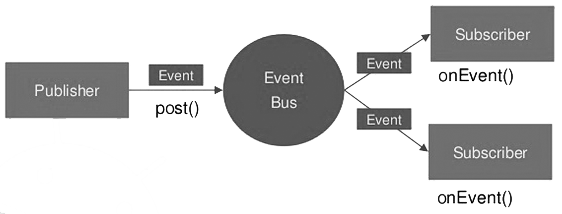
\includegraphics[width=0.6\textwidth]{publish_subscribe.png}}
	\caption{Publish / subscribe with the event bus.}
	\label{fig:publish_subscribe}
\end{figure}

\begin{listing}[!h]
	\centering
	\begin{tabular}{c}
		\begin{lstlisting}[language=java]    
@Override
public void onStart() {
    super.onStart();
    EventBus.getDefault().register(this);
}

@Override
public void onStop() {
    EventBus.getDefault().unregister(this);
    super.onStop();
}

// This method will be called when a MessageEvent is posted
public void onEvent(MessageEvent event){
    doSomethingWith(event);
}
		\end{lstlisting}    
 	\end{tabular}
	\caption{Register and unregister from the \textit{EventBus}.}
	\label{lst:eventbus_reg_unr}
\end{listing}

Last but not least, a simple line is used to post an event from any part of the code. All subscribers matching the event type will receive it:
\begin{lstlisting}[language=java]
EventBus.getDefault().post(new MessageEvent("Hello everyone!"));
\end{lstlisting}

\section{Data management}

\subsection{Reload the data}
On the right hand side of the header bar, a button gives the option to reload the data. This is handled in the \texttt{BaseActivity} class. The content of the activity disappears while the task is processed, and a loading animation layout is shown.\\

The reload from our server is composed of two steps. First, the user information and the associated sensors are updated. Then, the values and the statistics corresponding to each sensor owned by the user are updated. As far as the values are concerned, only the new ones are downloaded.

\subsubsection{Communication with the server}
Each operation between the server and the client uses our Java API. To communicate with the server, the \texttt{RestTemplate} class of \textit{Spring Web} is used. It easily handles HTTP requests (GET, POST, DELETE...) to the RESTful services. The conversion between JSON and Java objects is handled by \textit{Jackson}, a tool used for mapping the two. Each request is conducted in a separate thread with the help of an AsyncTask.\\

Regarding security, a static method from \texttt{CryptoUtils} creates the basic authentication headers for each request. They are added to the \texttt{RestTemplate} before sending the request.

\subsection{Off-line synchronization}
To ensure off-line usage, the data fetched from the server are synchronized in a \textit{SQLite} database on the mobile device. The structure of this database is quite simple because very little information needs to be stored. \textit{ORMLite} is used to store data that can be represented as objects (e.g. a sensor). Two controllers are used to store the data associated to a user and to the statistics. A particular object, \texttt{SensorValueDao}\footnote{The Data Access Object (DAO) pattern is used to separate low-level data accessing API or operations from high-level business services \cite{DAO:online}.}  is used to store the list of key-value pairs associated with a sensor. \\

A class called \texttt{DatabaseHelper} was built on top of \textit{ORMLite} to handle the creation, upgrade and deletion of tables. It has also getters for the different types of values. 

\section{Configuration, SingleInstance and util classes}
The file \texttt{Config.java} groups important global settings of the application. For example, the \texttt{SENDER\_ID} used with the notification system, the public server address, the port and protocol used to communicate with the server, etc.\\

The class \texttt{SingleInstance} groups objects with exactly one instance by using the Singleton pattern. For example, the \texttt{DatabaseHelper} is available from \texttt{SingleInstance} as it is accessed in different parts of the mobile application.\\

Moreover, for practical reasons, generic static methods that are not related to a particular object were placed in a package called \texttt{util}. Amongst those classes, one is particularly interesting and is described below.

\subsubsection{LogUtils}
This class is a wrapper around the log system of \textit{Android} to provide a “debug mode” within the application. \texttt{LogUtils} provides multiple log levels that are correctly prefixed with “\texttt{myconsumption\_}” (similar to all Google applications). The different levels are: debug; verbose; info; warning; and error. The debug mode is set in the \texttt{Config} class with a boolean variable (when set to false, verbose and debug logs are not shown). We used this system in every new part of the application with the appropriate level. An illustration of this is given in Figure \ref{fig:logs}.

\begin{figure}[htbp]
	\centerline{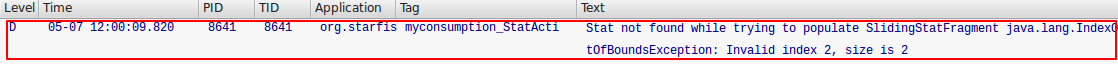
\includegraphics[width=1\textwidth]{logs.png}}
	\caption{How the logs are displayed in the \textit{Android Device Monitor}.}
	\label{fig:logs}
\end{figure}

\section{Notifications}
The notification system has been fully detailed in a section about the server implementation. As far as the mobile application is concerned, one of the first things done by the \texttt{BaseActivity} class is to check if the \textit{Google Play Services} are available on the device. If so, they are used to contact the \textit{Google Cloud Messaging} server. A specific class was created for this purpose: \texttt{GCMRegister.java}. It is based on the \textit{Android} Documentation: \href{https://developer.android.com/google/gcm/client.html}{Implementing GCM Client on \textit{Android}}. \\

When the application is launched for the first time, the \texttt{GCMRegister} sends the \texttt{SENDER\_ID} specific to \textit{MyConsumption} to the GCM server for registration. After successful registration, the GCM server returns a \texttt{REGISTRATION\_ID} to the mobile device. This ID is sent to our server and will be used to send a notification message to this specific device.\\

Finally, two classes are involved in the process of receiving a notification. The first is the \texttt{GCMBroadcastReceiver} which extends \texttt{WakefulBroadcast-} \verb!Receiver!. It is a special type of broadcast receiver that creates and manages a partial wake lock for the application. It has only one function (\texttt{onReceive()}) called when a notification is triggered and which loads the second class involved in this process: \texttt{GCMIntentService}.  The latter is in charge of creating the notification on the device.\\

As this is implemented as a service defined in the \texttt{AndroidManifest} file of the application, notifications are shown even if \textit{MyConsumption} is not running (see Figure \ref{fig:notif_device}).
 
\begin{figure}[htbp]
	\centerline{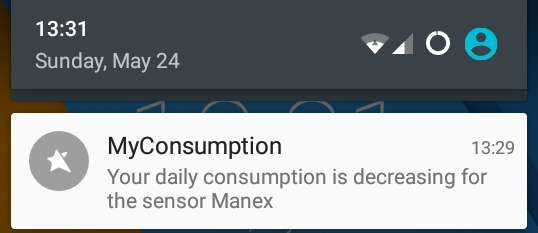
\includegraphics[width=0.5\textwidth]{notif_device.png}}
	\caption{A notification is showing up.}
	\label{fig:notif_device}
\end{figure}



\part{Tests and deployment}
\renewcommand\partcontent{TESTS AND DEPLOYMENT: }

\chapter{Tests}
This last part aims at discussing the different tests of the system as well as its deployment in a realistic practical environment. We start this discussion by assessing the design and the quality of the work done. After that, the different tests performed are described. Finally, the deployment of the system is detailed.

\section{Design validation}
The methodology followed to develop this software allowed us to be modular. Indeed, at regular intervals, we were able to review the work to tune and adjust its behavior accordingly. It helped us to keep our design valid along the way.\\

The features described in the design part of the document were all validated during one of the meetings with Antoine and Vincent. The graph smoothing, the statistics, the comparison, etc. were much discussed in a constructive spirit. They were only considered achieved after a positive feedback. The same applies to the user interfaces. Some details proposed in the description  of the design requirements could not be implemented but workarounds\footnote{These workarounds were discussed in the implementation part of the work.} were found during the meetings. For both the features and the user interfaces, the results are conclusive.\\
As far as the use cases are concerned, their testing involves creating test cases based on the use cases. Thus, the quality of the work done was assessed by following their usage description on the real application in order to test the validity of their functional requirements. \\ 

Regarding the modularity of the system, we focused on several concerns. Firstly, the two build automation tools\footnote{Maven for the server and Gradle for the mobile application.} used allow to easily deploy the code by other developers. Secondly, the design of the smart meter data retriever allows to easily add new types of sensors by using a strong Object-Oriented approach. Thirdly, thanks to the Java API it provides, the server is completely independent of the mobile application; an update does not affect the clients. Finally, in the \textit{Android} application, the way activities extend the \texttt{BaseActivity} is also modular regarding the common features shared by these activities.

\section{Software testing}
Of course, during development, the first thing we do is to run our own programmer's “acceptance test”: we code, compile, and run \cite{junit:book}. This a daily process: when running the software, we test it. It may just be clicking a button to see if it triggers the expected action. Sometimes, the test is more significant. For example, adding, viewing, editing and deleting a record. But those tests are done, over and over again.\\

This approach is not the most reliable. It is a boring “random” repetitive work, often not consistent and which does not give precise results and information at the end. However, with the rise of \emph{Agile} and \emph{Test Driven Developments} movements, programmers are encouraged to write automated tests \cite{cleancode:book}. The following sections give an introduction to more specific tests with their application in this work.

\subsection{F.I.R.S.T.}
The book “Clean Code A Handbook of Agile Software Craftsmanship” \cite{cleancode:book} advises us to follow five rules (from  the above acronym) to write good tests.
\begin{itemize}
	\item \textit{Fast:} tests should be fast and run quickly (so that they can be run frequently and bugs are found early enough to be fixed easily);
	\item \textit{Independent:} tests should not depend on each other and one test should not set up the conditions for the next test (which means that one can run the tests in any order);
	\item \textit{Repeatable:} tests should be repeatable in any environment (in production, on one’s laptop...);
	\item \textit{Self-Validating:} tests should have a boolean output (either they pass or fail); 
	\item \textit{Timely:} tests need to be written in a timely fashion (before the production code that makes them pass).
\end{itemize}

\subsection{Unit tests}
A unit test examines the behavior of a distinct unit of work. Within a Java application, the “distinct unit of work” is often a single method \cite{junit:book}. It should have a very narrow and well defined scope. For those reasons, unit tests fit particularly well the F.I.R.S.T. principles described above. When such a test fails, it tells the programmer what piece of code needs to be fixed.\\

In this work, on the server side,  we  made simple unit tests with \textit{JUnit} (an effective open source unit testing framework for Java). For this purpose, the \texttt{spring-} \verb!boot-starter-test! dependency was used. Three actions of the server were tested:
\begin{itemize}
	\item Access a non-protected RESTful resource;
	\item Access a protected RESTful resource;
	\item See if the database can be accessed.
\end{itemize}

Under the folder  \texttt{src/main/test} of the server, three classes implement the tests described above: \texttt{ConfigControllerTest}, \texttt{UserControllerTest}, \texttt{User-} \verb!RepositoryTest! respectively. They are all based on the same scheme: they used the annotation \texttt{@RunWith} (\texttt{SpringJUnit4ClassRunner.class}) which tells that the class will be used for a unit test. Moreover, each test is divided in two parts: first a setup which is made and then each unit test. \textit{IntelliJ IDEA} (the IDE used in this work) can be configured to handle the running configuration for the tests. A result of a test is illustrated on Figure \ref{fig:tests}.

\begin{figure}[htbp]
	\centerline{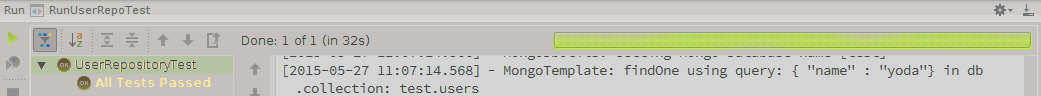
\includegraphics[width=1\textwidth]{tests.png}}
	\caption{A successful unit test in \textit{IntelliJ IDEA}.}
	\label{fig:tests}
\end{figure}

Of course, one could extend those tests to ensure reliable operations of the server on a production machine. To go even further, a continuous integration software could be used to test the proper functioning of the system deployed. Tools like \textit{TeamCity} or \textit{Jenkins} could be appropriate. But the goal of the approach here was to prove that unit tests are easy to implement regarding the design of the server, which is the case.

\subsection{Integration tests}
The purpose of these tests is to verify the correct inter-operation of multiple subsystems. It includes different levels, from testing integration between two classes, to testing integration with the production environment. When it fails, it tells you that the pieces of the application are not working together as expected. Such tests are addressed in the next chapter of this document, where we describe the deployment of the system.

\subsection{Functional tests}
Functional tests involve testing the system as a black box. It checks a particular feature for correctness by comparing the results for a given input against the specification. We  have not made such tests in an automated fashion (even if some debug logs provide information about the output of some methods). Nevertheless, while debugging, functions and methods have been tested by checking the value they returned. 

\subsection{Acceptance tests}
Acceptance tests ensure that the functionality meets their requirements. They were done along the way during the meetings with Antoine and Vincent to check if a feature or a use case was correctly implemented. It is similar to an integration test, but with a focus on the use case rather than on the components involved. When such a test fails, it means that the application is not doing what the customer expects it to do.  

\subsection{Regression tests}
After integrating a new feature (or maybe fixing one), the programmer should run the unit tests again. This \emph{regression testing} process ensures that further changes have not broken any units that were already tested. When these tests fail, it means that the application no longer behaves the way it used to.

\chapter{Deployment}
As an integral part of the tests, the deployment of the system was a good opportunity to see if it really works in a realistic practical environment. It involves:
\begin{itemize}
	\item Two \textit{Flukso} smart meters: one in the office of the company and another at home\footnote{Since the energy consumption of the company “Manex” is greater than my home's one, the data of sensor “Ans” are not easy to see...};
	\item A virtual machine to deploy the server accessible with a public IP;
	\item Several \textit{Android} devices running the API 16 and 21 of the OS.
\end{itemize}		

The smart meters are easy to set up. Once connected to one’s internet connection and to the electrical meter, they send their data to the \textit{Flukso} server. Then, we can associate them to the mobile application so that our back end will fetch and process the data (see Figure \ref{fig:chart}). As far as the server deployment is concerned, the process is quite straightforward. It is fully detailed in the Appendix of this document. 

\begin{figure}[htbp]
	\centerline{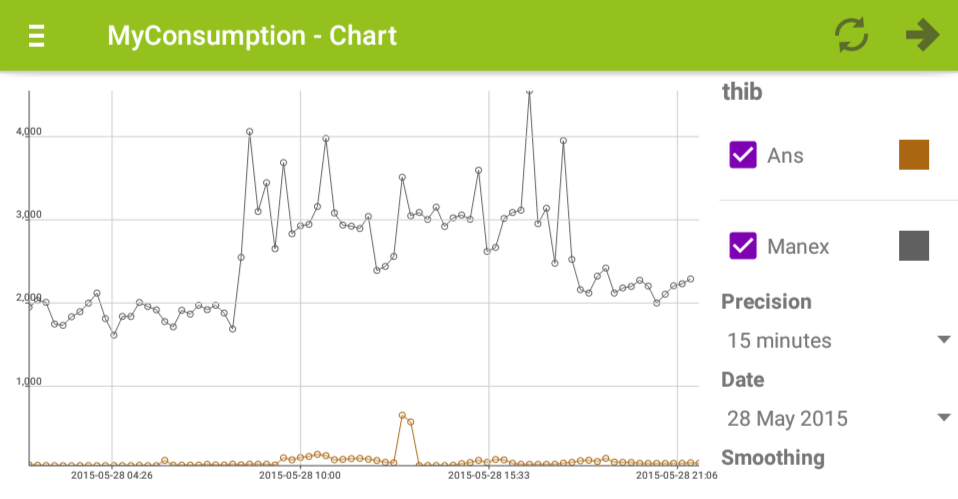
\includegraphics[width=0.7\textwidth]{chart.png}}
	\caption{The two smart meters in the mobile application.}
	\label{fig:chart}
\end{figure}


The result gives us an operating server accessible anywhere. This configuration suits individuals who can easily use the system just by installing the app and a smart meter at home. For companies, the simple deployment of the server in a practical environment allows them to easily use this project. Several devices were used to test the app this real world environment. In the end, the results are conclusive.



\part{Conclusion and future work}
\renewcommand\partcontent{CONCLUSIONS: }

\chapter{Conclusion}
In the introduction, we expressed the hope that the work in this master’s thesis could simplify and highlight the key steps of an energy monitoring system's implementation by providing a good working example. In this final part, we will conclude by describing the progress made towards this goal regarding our design implementation. We will also suggest some future directions that could provide the next steps in the development of this system. \\

The objective of this master’s thesis was to provide a mobile application for real-time energy consumption monitoring. This aim was motivated by the increase in energy efficiency measures where intelligent monitoring is an essential asset. Such an application could benefit both companies and individuals, as measuring energy consumption is the first step toward finding ways to decrease it.\\

The first part of the project was dedicated to the design of the system. From the data fetched by an existing retriever, we were able to provide relevant information displayed in an effective and user-friendly way. The system was naturally separated into two parts: a back end, a server built upon \textit{Spring Boot}, and a front end, a mobile \textit{Android} application. Use cases, user interfaces and different features were investigated.\\

The system’s implementation was the core of the work. Particular attention was given  to the issues involved in the synchronization, distribution and backup of energy consumption data. As a result of the design guidelines drafted in the first chapters, the users of \textit{MyConsumption} can now check their power consumption in many different ways, including a line chart of their consumption, a set of statistics about their past day, week, month and year’s consumption or even a comparison with an average customer profile. Moreover, responses to abnormal cases have been implemented. The communication between the application and the server was the crux of the matter, and special care to secure the exchanges was taken.\\

During the last part of the project, we focused on testing and validating the system for every feature and use cases investigated. Different types of tests have been made at different levels. As far as the back end is concerned, specific unit tests are implemented as a proof of concept of their technical feasibility.\\

On the other hand, the last phase of the project also revealed some limitations and drawbacks to the system. The consumption profiles given in the comparison feature are not as accurate as expected. We were faced with a lack of comparable information needed to achieve more precise standard profiles. On the server side, our initial idea to retrieve prices and electricity information could not be implemented given the resources found, and consequently a workaround had to be considered. Lastly, the security layer added to the system is a good first step, but it should be developed further. \\

Finally, by covering a wide range of features, this work has opened the door to other perspectives on future development. Many ideas, such as porting the application to another platform, adding intelligence to the system, and controlling electrical appliances are given in the next section to possibly complete the present working monitoring system.\\

At the close of the project, my personal opinion is that this work gives a good and extensible energy monitoring system in view of the time allocated to design and set it up. It was a rich and interesting experience; I have learned and discovered many tools and frameworks in a short period of time. In terms of challenges, it was not easy to continue the work of another student. However, the help of the company team guided me through this process. Finally, the opportunity to have a professional working experience in the area of mobile development has been particularly valuable. I was positively surprised by the pleasant working atmosphere as well as the continued interest the company showed in my work.\\

In conclusion, even if this system still has some unavoidable drawbacks, they do not affect its functionality in any way; the development meets the requirements as defined in the project description and within the scope of this thesis.

\chapter{Suggestions for future work}
While drafting this document, many ideas and suggestions for future prospects came to our minds. This final section of the report starts by explaining what could be done if the development process was continued. We then recall features that could not be implemented, but which were drafted during the early meetings. Finally, other ideas and features of larger scope are suggested.

\section{Improvements to the current system}

\subsection{Logs}
The log system used for both server and client has been well implemented. As far as the back end is concerned, the library \texttt{slf4j} is used in many parts of the code. In the front end, a wrapper around the \textit{Android} log system is used to integrate the application. Those two systems are sound and complete. Nevertheless, some pieces of code that come from the previous version of the system do not use this log system. For overall consistency, it would be ideal to update them.

\subsection{Event bus}
At the end of the work, a good workaround to easily support internal communication in the mobile application was found. The Event Bus provides a better approach and facilitates the communication between every part of the application. As for the log system, it is not implemented in some old pieces of the code (a few \texttt{Async tasks}) that still use the old scheme with \textit{Android} callbacks. This is not a drawback since it works properly, but for consistency they could also be updated.

\subsection{Security}
Security was discussed during the work. The basic authentication mechanism over SSL provide a good layer of security. Nevertheless, some weaknesses of this approach have been discussed. The password is stored without salt, HTTPS is not in place because of the missing certificate and some design choices may not be the best. 

\section{Features not implemented}
Having sketched the features of the mobile application during the first meetings, we then prioritized them. Sadly, two features that were discussed to be implemented at first sight did not get the chance to be developed to completion. 

\subsection{Evolution of consumption}
Based on the idea that a user’s consumption could be impacted by a change in habit or behavior, we wanted the user to understand how their consumption evolves. The graph available on the main screen of the application already gives him/her a good idea of this. To take the analysis a few steps further, two things were suggested regarding the evolution of consumption: 
\begin{itemize}
	\item Let the user the option to enter a comment on the graph at a given time;
	\item Estimate the energy consumption and cost at the end of a period (e.g. a month) by extrapolation.
\end{itemize}
The first feature could be implemented by tweaking the chart library while the second could be achieved with forecasts of data based on a polynomial extrapolation, or using a moving average.

\subsection{Manual consumption reading}
Some people have a look at their electricity meter more than once a year. By allowing the user to enter their consumption manually, one could target those who do not have a smart meter. As it is not very likely that someone would use the mobile application this way, this feature was not made a priority and was left for a possible future work.

\section{Features of larger scope }

\subsection{Add intelligence to the system}
For now, \textit{MyConsumption} is only a monitoring system. As pointed out in the introduction, many existing systems are integrated into larger environments. The tool developed in this work could be extended to be more specific. Below are some ideas.

\subsubsection{Control electrical appliances}
Most of the systems described in the introduction control a domestic heating system. Similarly, \textit{MyConsumption} could be extended to interact with an existing thermostat. Other electrical appliances, such as a dishwasher, could also be added into the mix thanks to existing remote controlled sockets.

\subsubsection{External data}
Along the same line of thinking, \textit{MyConsumption} could base its predictions on external data in order to be more relevant. For example, one could extend the analysis we already provide with the localization of the user. Moreover, the evolution of the consumption could take into account weather forecasts to estimate the energy consumption in the near future. Finally, some existing systems try to learn from the habits of the user. This could also be applied to \textit{MyConsumption} (see the \textit{Nest} thermostat by Google, for example). 

\subsection{Server database running on clusters}
\textit{MongoDb}, the database used in this work, is specifically designed to run well on clusters. With many clients, this possibility might be envisaged to balance the traffic loads. Patrick Herbeuval (who worked on this project last year) already gave this some thought, but this could be further developed.

\subsection{Automated invoices}
By assuming a system with many clients, a power supplier could provide an automated invoice processing software. This could replace the current archaic system where we have to note manually our annual consumption on a sheet of paper and hang it in a window of our house.

\subsection{Smarter smart grid}
Power suppliers use smart grids to optimize the efficiency of the production and distribution of electricity.  With a monitoring system and access to the exact consumption data of every single customer, the smart grid could be more accurate, leading to large-scale savings. This idea could be expanded as well.

\subsection{Target other platforms}
\textit{MyConsumption} is only available on the \textit{Android} platform. One could see the value in porting the software to another platform (such as iOS for Apple mobile devices), and/or to a web interface for online reading purposes.
 



\part{Appendices}
\renewcommand\partcontent{APPENDICES: }

\chapter{Mobile application's UI}

\begin{figure}[htbp]
	\centerline{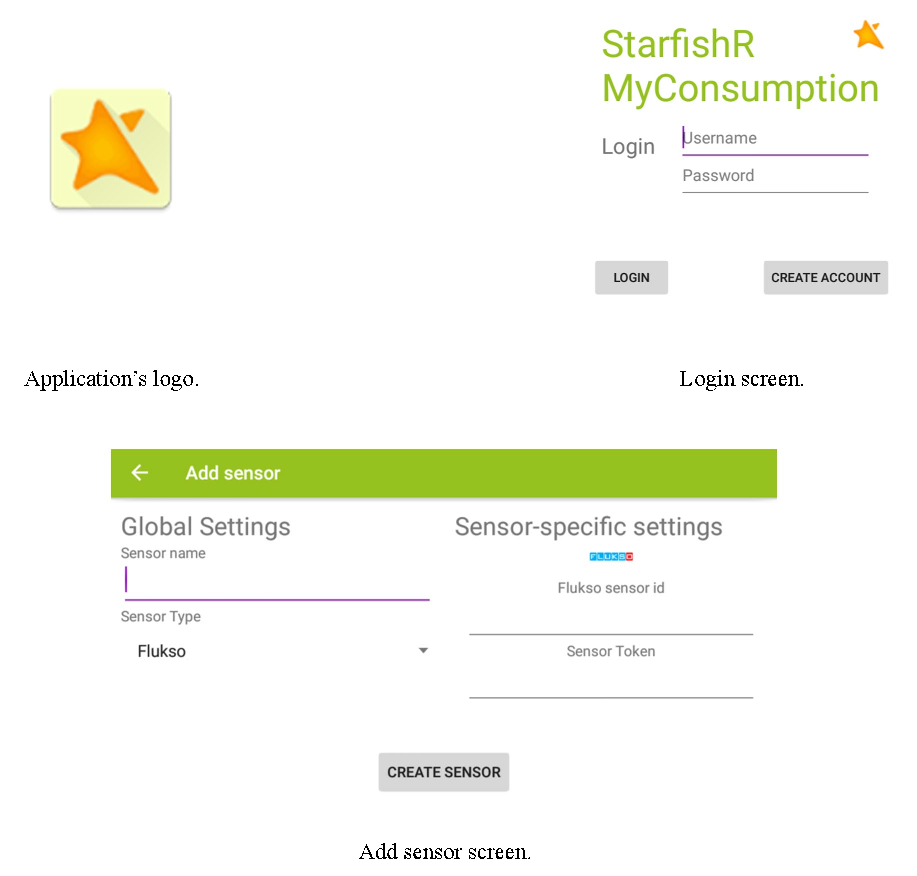
\includegraphics[width=1\textwidth]{screenshot1.pdf}}
	\caption{Logo, login and add sensor.}
	\label{fig:screenshot1}
\end{figure}

\begin{figure}[htbp]
	\centerline{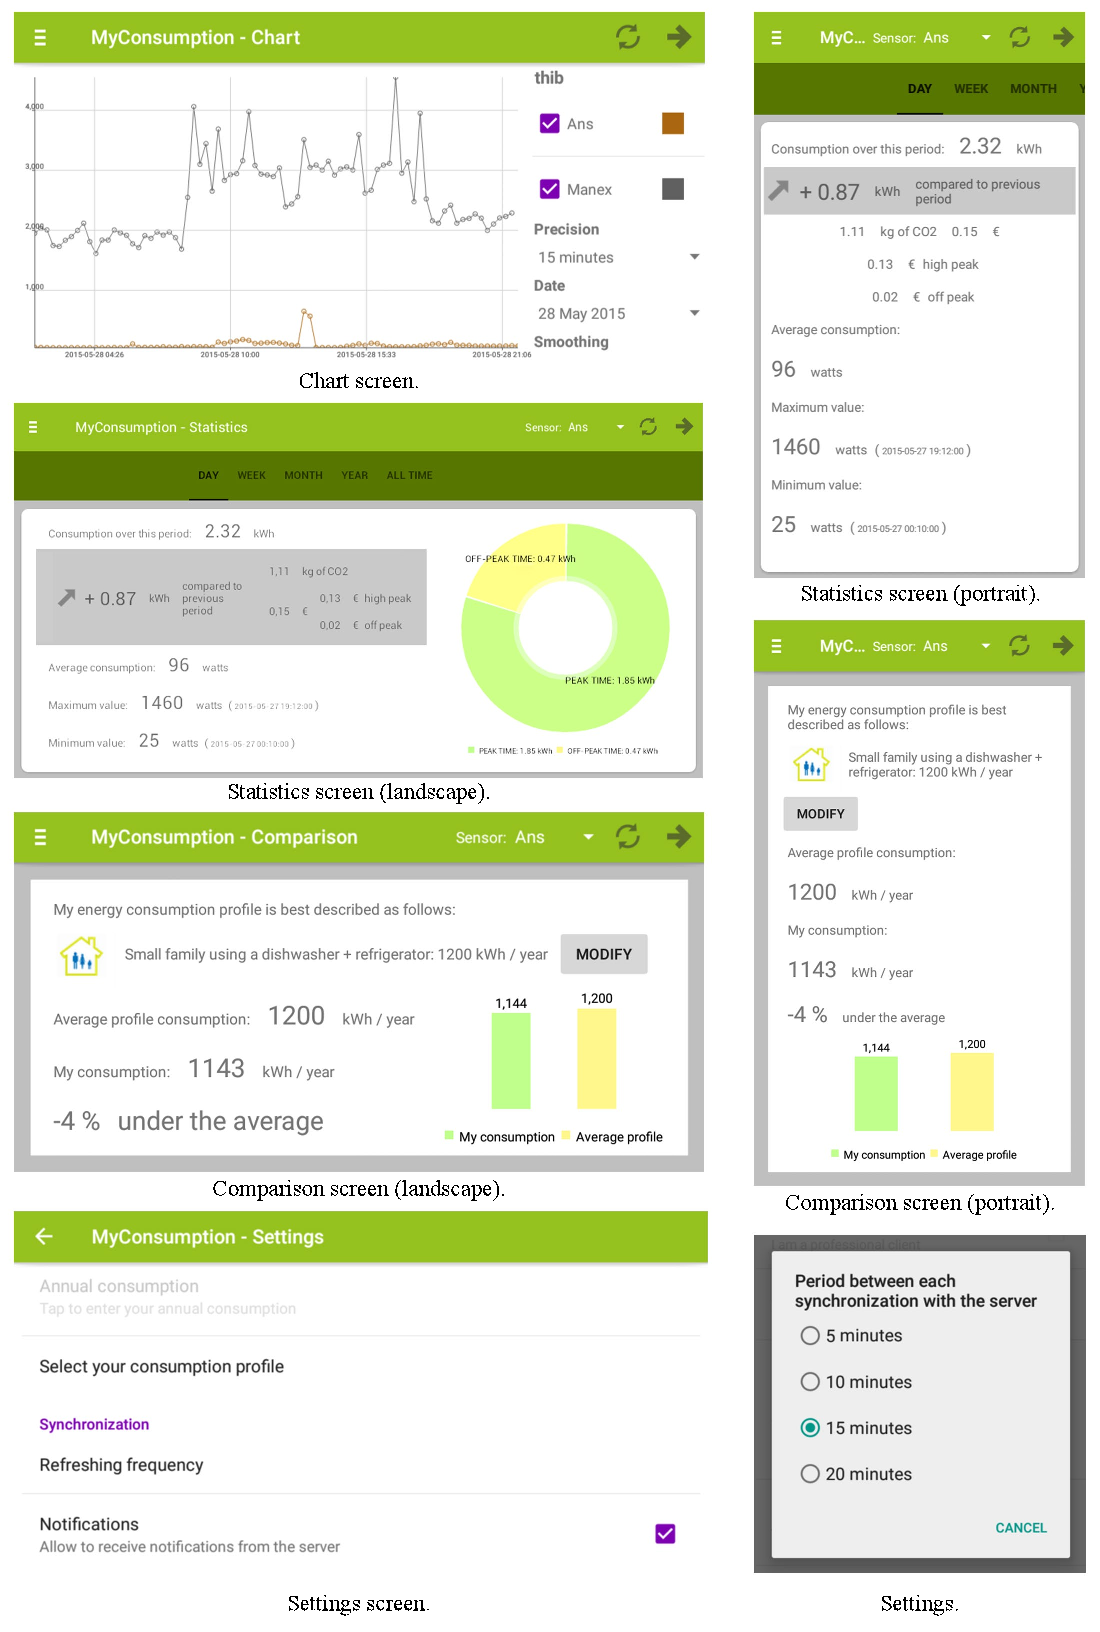
\includegraphics[width=1\textwidth]{screenshot2.pdf}}
	\caption{Chart, statistics, comparison and settings.}
	\label{fig:screenshot2}
\end{figure}

\chapter{Deployment of the system}

\section*{Setup}
A specific virtual machine (running Debian 7.8 \textit{Wheezy}) is dedicated to host our server. An SSH tunneling and specific ports forwarding were configured so that programmers and clients can access the machine from anywhere. Finally, \textit{Tomcat 8} and \textit{MongoDb 3} were installed on the machine.\\

As far as the configuration of the server is concerned, we had to add the following dependency to inform \textit{Spring Boot} that \textit{Tomcat} is running on the virtual machine:
\begin{lstlisting}[breaklines]
	<dependency>
	    <groupId>org.springframework.boot</groupId>
	    <artifactId>spring-boot-starter-tomcat</artifactId>
	   <scope>provided</scope>
	</dependency>
\end{lstlisting}

\section*{Deployment}
The process to deploy the server is quite straightforward. First, we run the \textit{Maven} command: \texttt{mvn package} which builds a self-contained \texttt{WAR} file.\\

Next, we can clean the virtual machine (if an older version of the back end was already deployed). The following commands are used:
\begin{itemize}
	\item \texttt{ssh thibaud.ledent@212.166.22.110}
	\item \texttt{rm /home/thibaud.ledent/my-consumption-business-1.0.0-} \\ \verb!SNAPSHOT.war!
	\item \texttt{rm /var/lib/tomcat8/webapps/ROOT.war}
	\item \texttt{rm -r /var/lib/tomcat8/webapps/ROOT}
	\item \texttt{rm /var/log/tomcat8/*}
\end{itemize}
After that, we need to transfer the \texttt{WAR} from the programmer’s machine to the virtual one: 
\begin{itemize}
	\item \texttt{/path/to/WAR/my-consumption-business-1.0.0-SNAPSHOT.war} \\ \verb!thibaud.ledent@212.166.22.110:/home/thibaud.ledent!
\end{itemize}
Finally, we can move the \texttt{WAR} to the dedicated folder of \textit{Tomcat} and restart it:
\begin{itemize}
	\item \texttt{ssh thibaud.ledent@212.166.22.110}
	\item \texttt{sudo su}
	\item \texttt{mv /home/thibaud.ledent/my-consumption-business-1.0.0-} \\
	\verb!SNAPSHOT.war /var/lib/tomcat8/webapps/ROOT.war!
	\item \texttt{/etc/init.d/tomcat8 restart}
\end{itemize}
Two other commands may be useful to display the logs:
\begin{itemize}
	\item \texttt{cat /var/log/tomcat8/catalina.out}
	\item \texttt{tail -f /var/log/tomcat8/catalina.201*-**-**.log}
\end{itemize}

\chapter{REST API Documentation}
The documentation below explains how to access our RESTful API to create, read, update and delete consumption data stored on the server. This API is available at \url{http://myconsumption.s23y.com}.

\section*{Configurations}
\subsection*{Ecological footprint}
\textbf{Path} /configs/co2 \\
\texttt{GET} request that returns the number of kg of \(CO_2\) corresponding to one kWh.

\subsection*{Peak price}
\textbf{Path} /configs/day \\
\texttt{GET} request that returns the price (in \euro ) of one kWh during the day.

\subsection*{Off-peak price}
\textbf{Path} /configs/night \\
\texttt{GET} request that returns the price (in \euro ) of one kWh during the night.

\section*{Notifications}
\textbf{Path} /notifs/\{\textit{name}\}/id/\{\textit{registerId}\} \\
\texttt{POST} request to set the register id of a user. \\
Path arguments:
\begin{itemize}
    \item \texttt{name}: String
    \item \texttt{registerId}: String
\end{itemize}

\section*{Sensors}
\subsection*{Get all sensors}
\textbf{Path} /sensors \\
\texttt{GET} request that returns an array of JSON objects each one representing a \texttt{Sensor-} \verb!DTO!.

\subsection*{Get a sensor}
\textbf{Path} /sensors/\{\textit{sensorId}\} \\
\texttt{GET} request that returns a JSON object representing a \texttt{SensorDTO}. \\
Path arguments:
\begin{itemize}
    \item \texttt{sensorId}: String
\end{itemize}

\subsection*{Get the values of a given sensor}
\textbf{Path} /sensors/\{\textit{sensorId}\}/data \\
\texttt{GET} request that returns a list of pairs values. \\
Path arguments:
\begin{itemize}
    \item \texttt{sensorId}: String
\end{itemize}
Request arguments:
\begin{itemize}
	\item \texttt{start}: int (optional, default value = 0)
	\item \texttt{end}: int (optional, default value = 0)
\end{itemize}

\subsection*{Create a new sensor}
\textbf{Path} /sensors/ \\
\texttt{POST} request to create a new sensor. \\
Path arguments:
\begin{itemize}
	\item \texttt{type}: String (default value = "")
	\item \texttt{settings}: String (default value = "")
	\item \texttt{name}: String (default value = "")
	\item \texttt{user}: String (default value = "")
\end{itemize}
\textit{Example:}
\begin{lstlisting}[breaklines]
{
	"type": "flukso",
	"settings": "{"token":"1d9bcb0d712c3c3266369dd6afdec14f", "fluksoId":"9337af875dba89f84a362d44070a2ecf"}",
	"name": "S23Y",
	"user": "thib"
}
\end{lstlisting}

\subsection*{Edit a sensor}
\textbf{Path} /sensors/{sensorId} \\
\texttt{POST} request to edit a sensor. \\
Path arguments:
\begin{itemize}
    \item \texttt{sensorId}: String
\end{itemize}
Request arguments:
\begin{itemize}
	\item \texttt{name}: String
	\item \texttt{settings}: String (default value = "")
\end{itemize}

\subsection*{Delete a sensor}
\textbf{Path} /sensors/\{\textit{sensorId}\} \\
\texttt{DELETE} request to delete a sensor. \\
Path arguments:
\begin{itemize}
    \item \texttt{sensorId}: String
\end{itemize}

\section*{Statistics}
\subsection*{Get all statistics}
\textbf{Path} /stats/sensor/\{\textit{sensorId}\} \\
\texttt{GET} request that returns an array of JSON objects each one representing a \texttt{StatDTO}.\\
Path arguments:
\begin{itemize}
    \item \texttt{sensorId}: String
\end{itemize}

\section*{Users} 
\subsection*{Get a user}
\textbf{Path} /users/\{\textit{name}\} \\
\texttt{GET} request that returns a JSON object representing a \texttt{UserDTO}.\\
Path arguments:
\begin{itemize}
	\item \texttt{name}: String
\end{itemize}

\subsection*{Create a user}
\textbf{Path} /users/\{\textit{name}\} \\
\texttt{POST} request  to create a new user.\\
Path arguments:
\begin{itemize}
	\item \texttt{name}: String
	\item \texttt{password}: String (default value = "")
\end{itemize}

\subsection*{Associate a sensor to a user}
\textbf{Path} /users/\{\textit{name}\}/sensor/\{\textit{sensorId}\} \\
\texttt{POST} request to associate a sensor to a user.\\
Path arguments:
\begin{itemize}
	\item \texttt{name}: String
	\item \texttt{sensorId}: String
\end{itemize}

\subsection*{Delete a user}
\textbf{Path} /users/\{\textit{name}\} \\
\texttt{DELETE} request to delete a user.\\
Path arguments:
\begin{itemize}
	\item \texttt{name}: String
\end{itemize}

\subsection*{Dissociate a sensor from a user}
\textbf{Path} /users/\{\textit{name}\}/sensor/\{\textit{sensorId}\} \\
\texttt{DELETE} request to dissociate a sensor from a user.\\
Path arguments:
\begin{itemize}
	\item \texttt{name}: String
	\item \texttt{sensorId}: String
\end{itemize}

\chapter{Meeting reports}
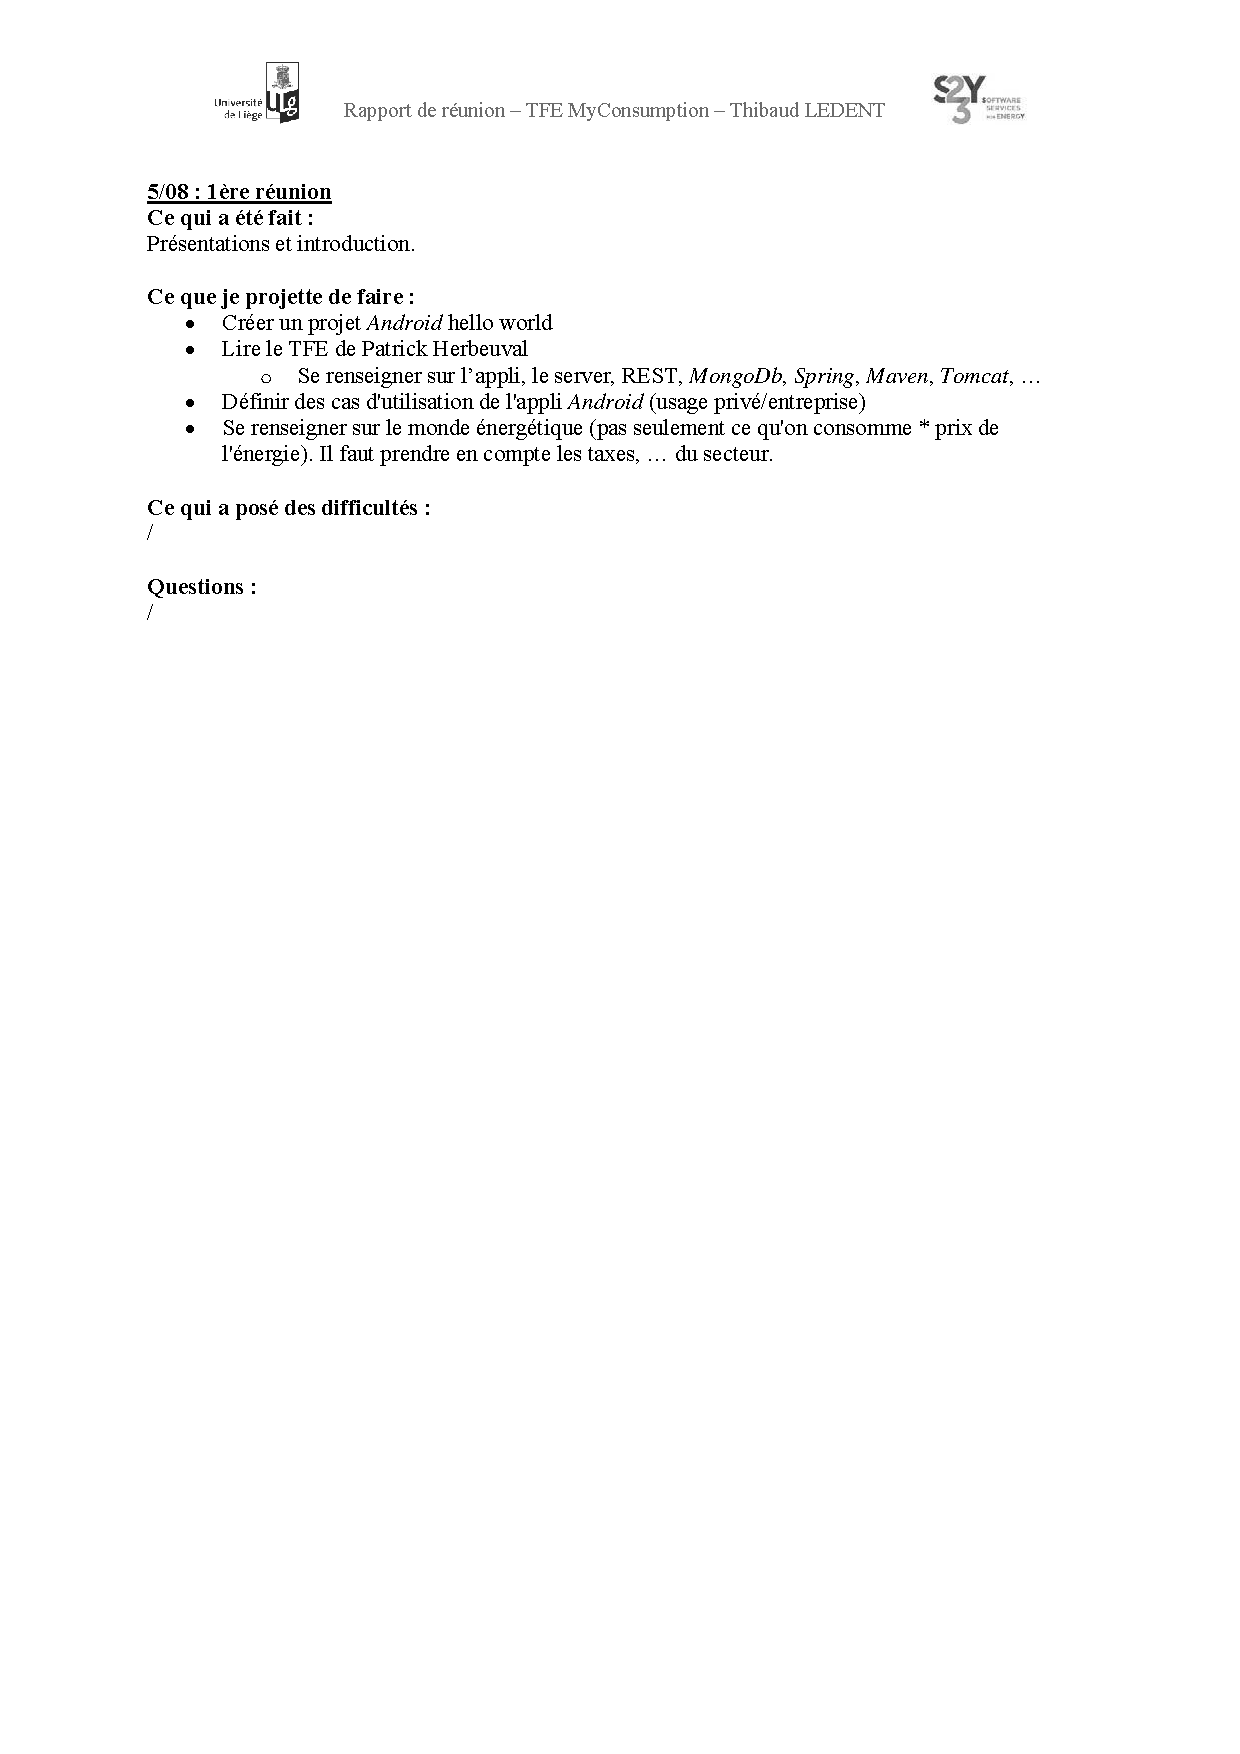
\includegraphics[width=1\textwidth]{reports_NB_Part1.pdf}
\newpage
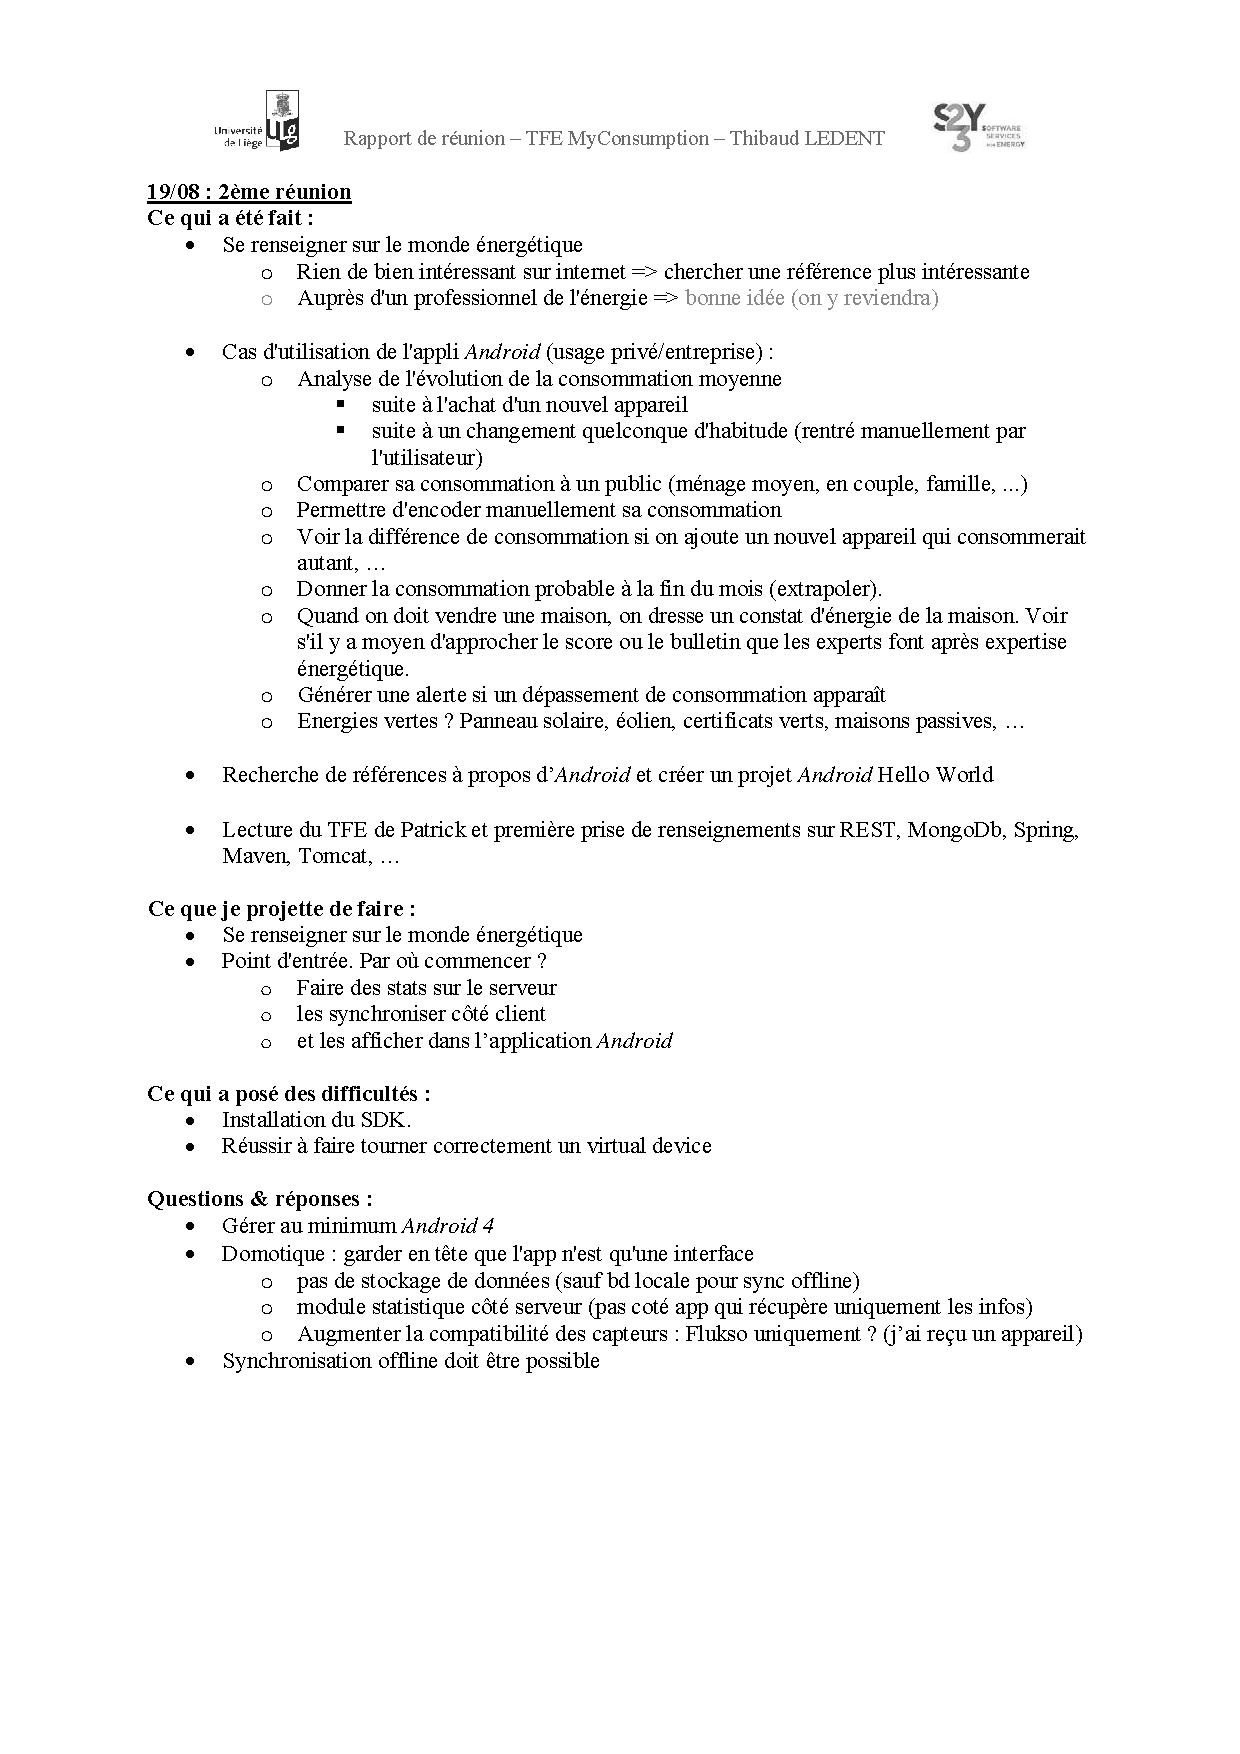
\includegraphics[width=1\textwidth]{reports_NB_Part2.pdf}
\newpage
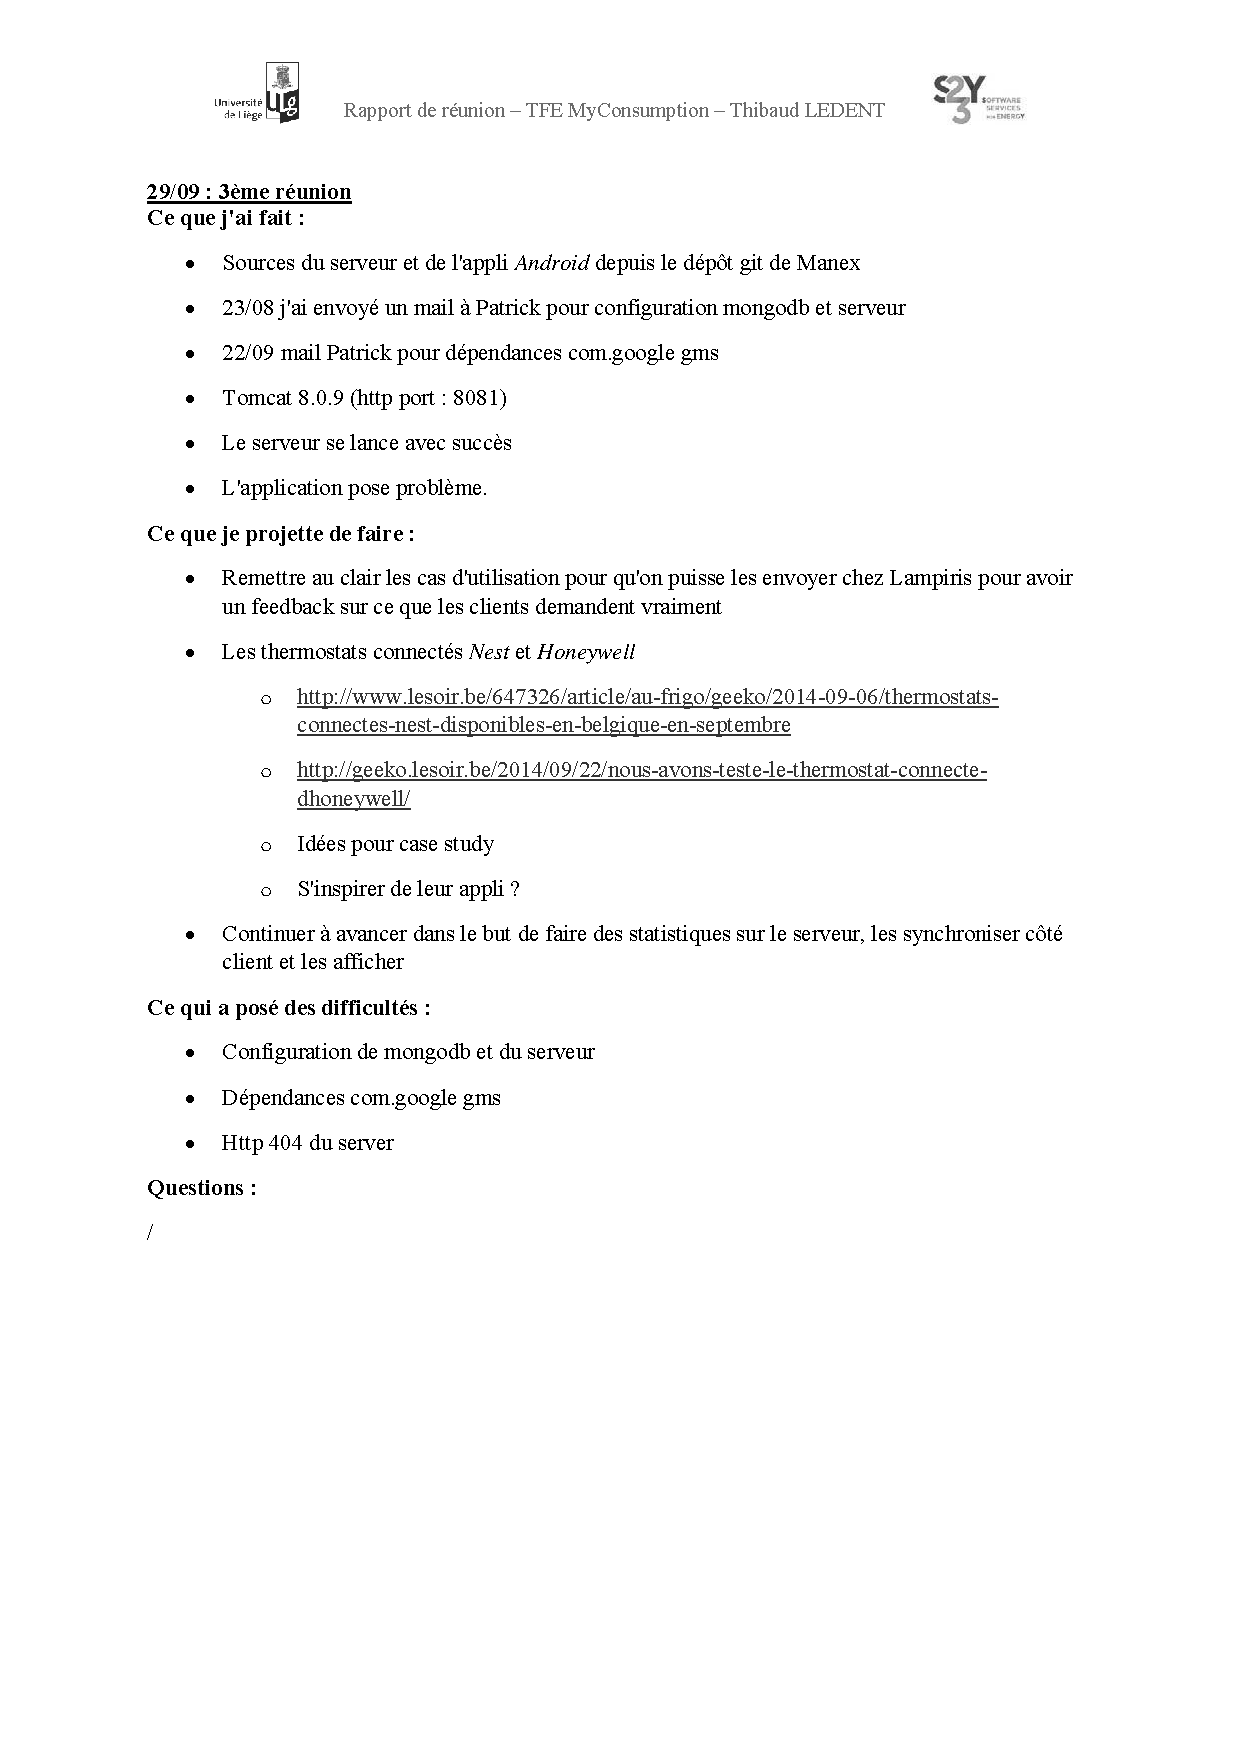
\includegraphics[width=1\textwidth]{reports_NB_Part3.pdf}
\newpage
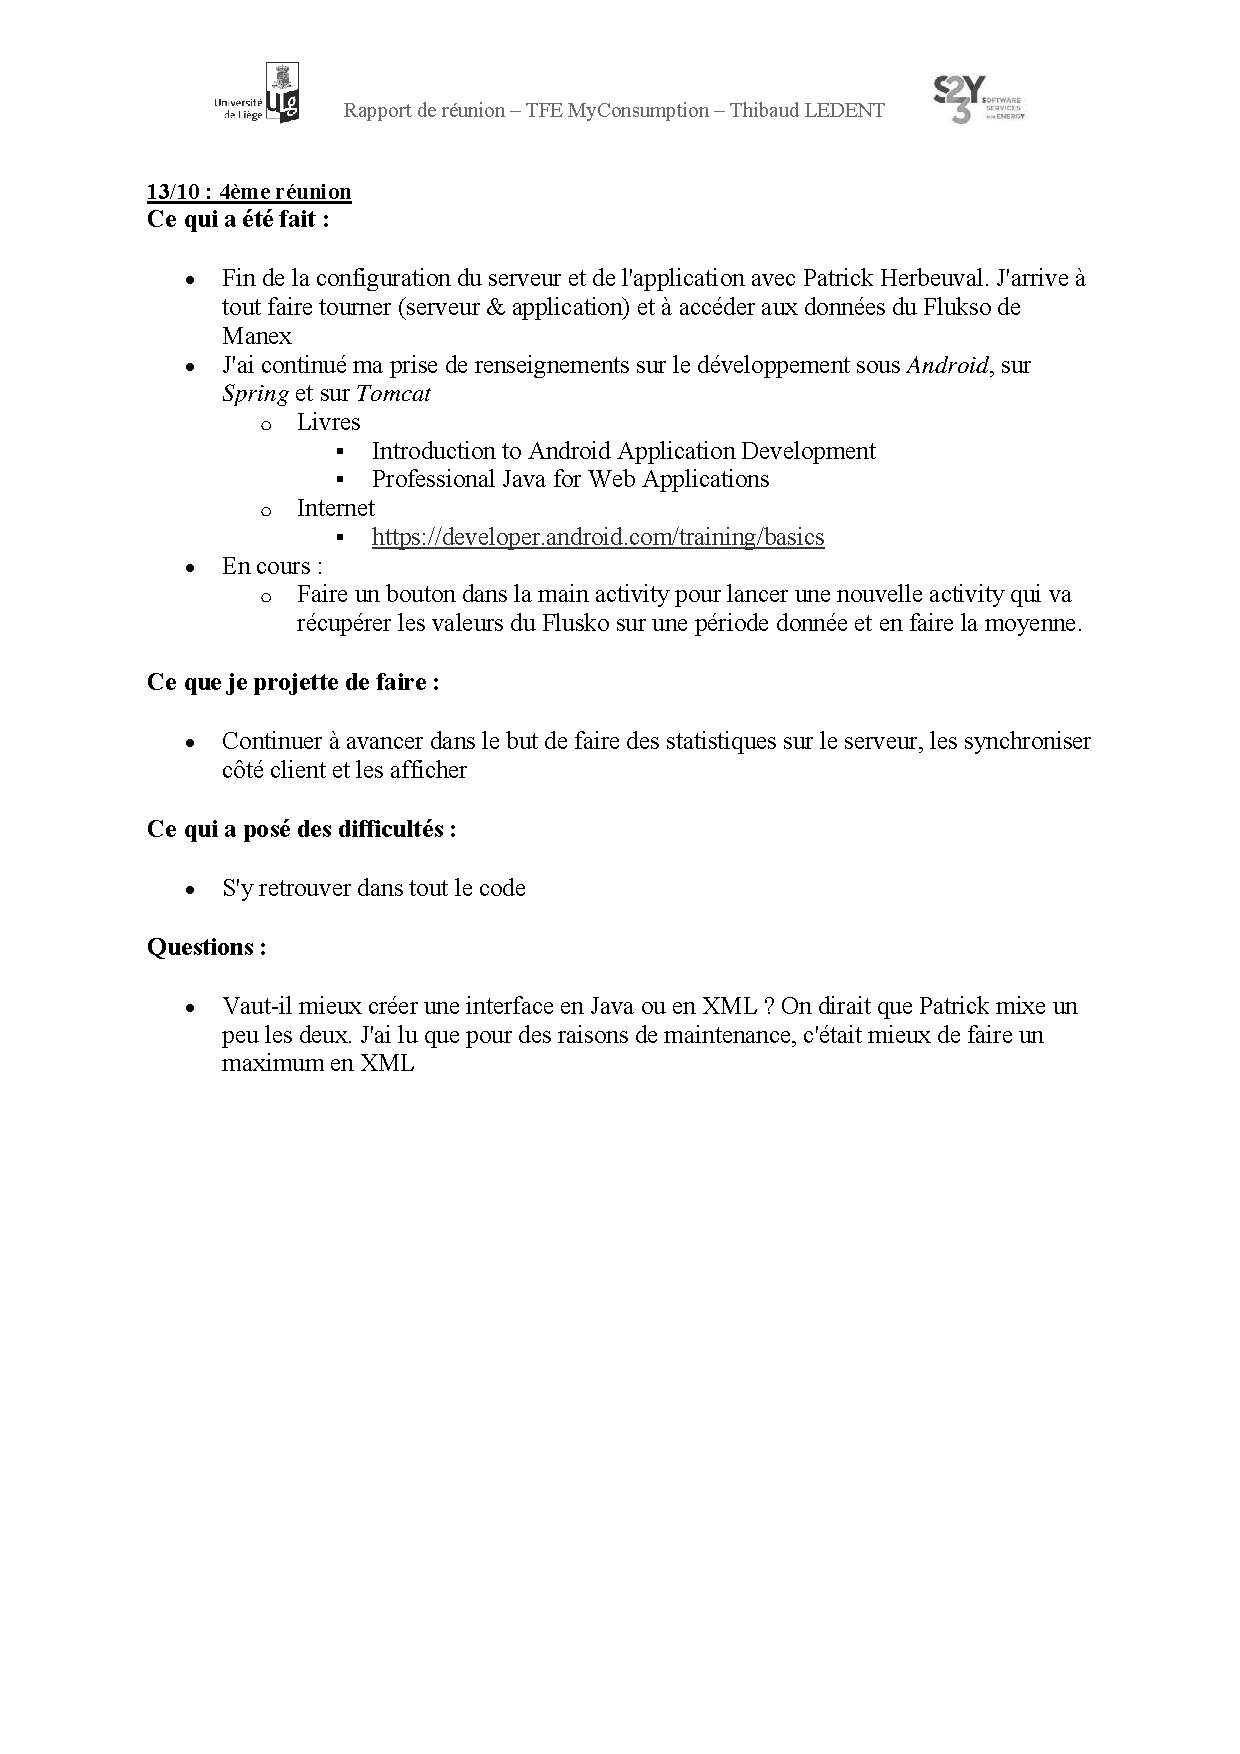
\includegraphics[width=1\textwidth]{reports_NB_Part4.pdf}
\newpage
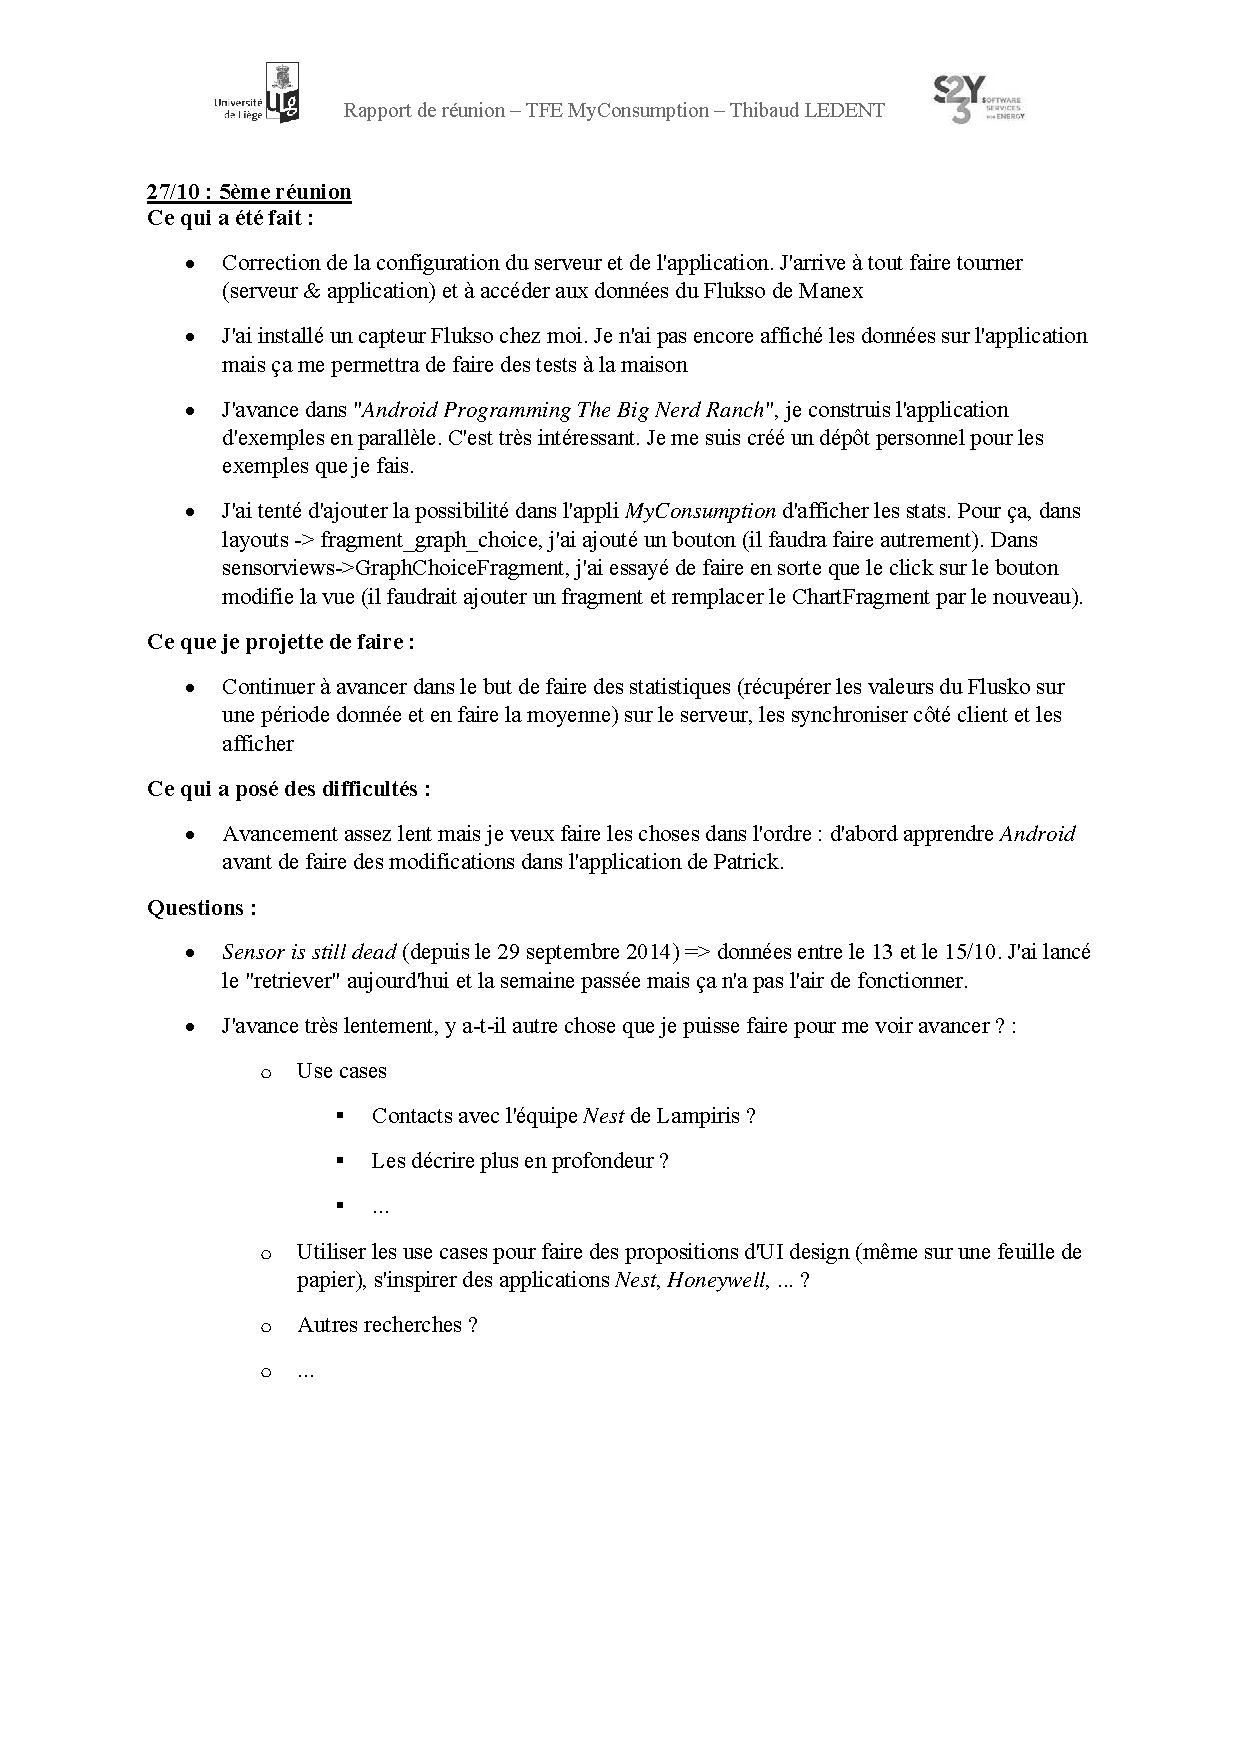
\includegraphics[width=1\textwidth]{reports_NB_Part5.pdf}
\newpage
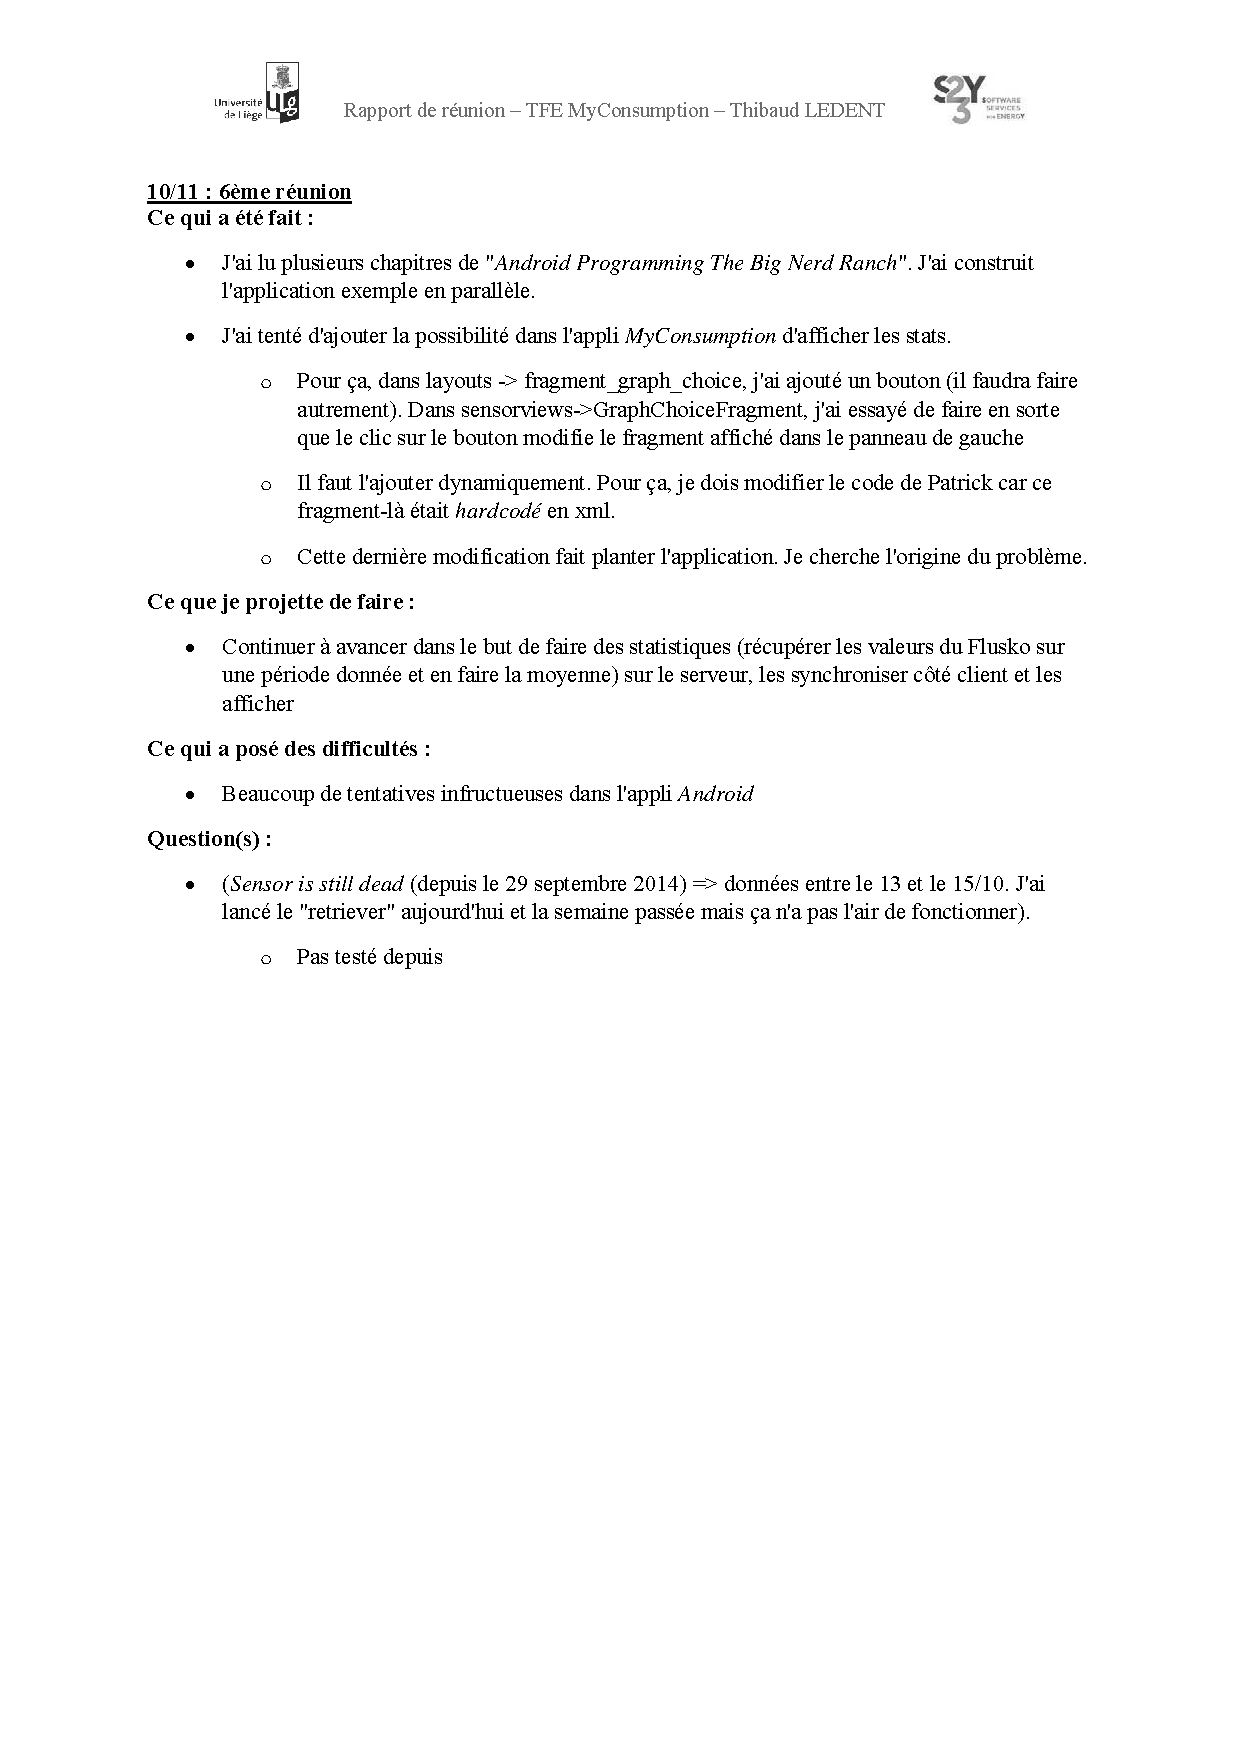
\includegraphics[width=1\textwidth]{reports_NB_Part6.pdf}
\newpage
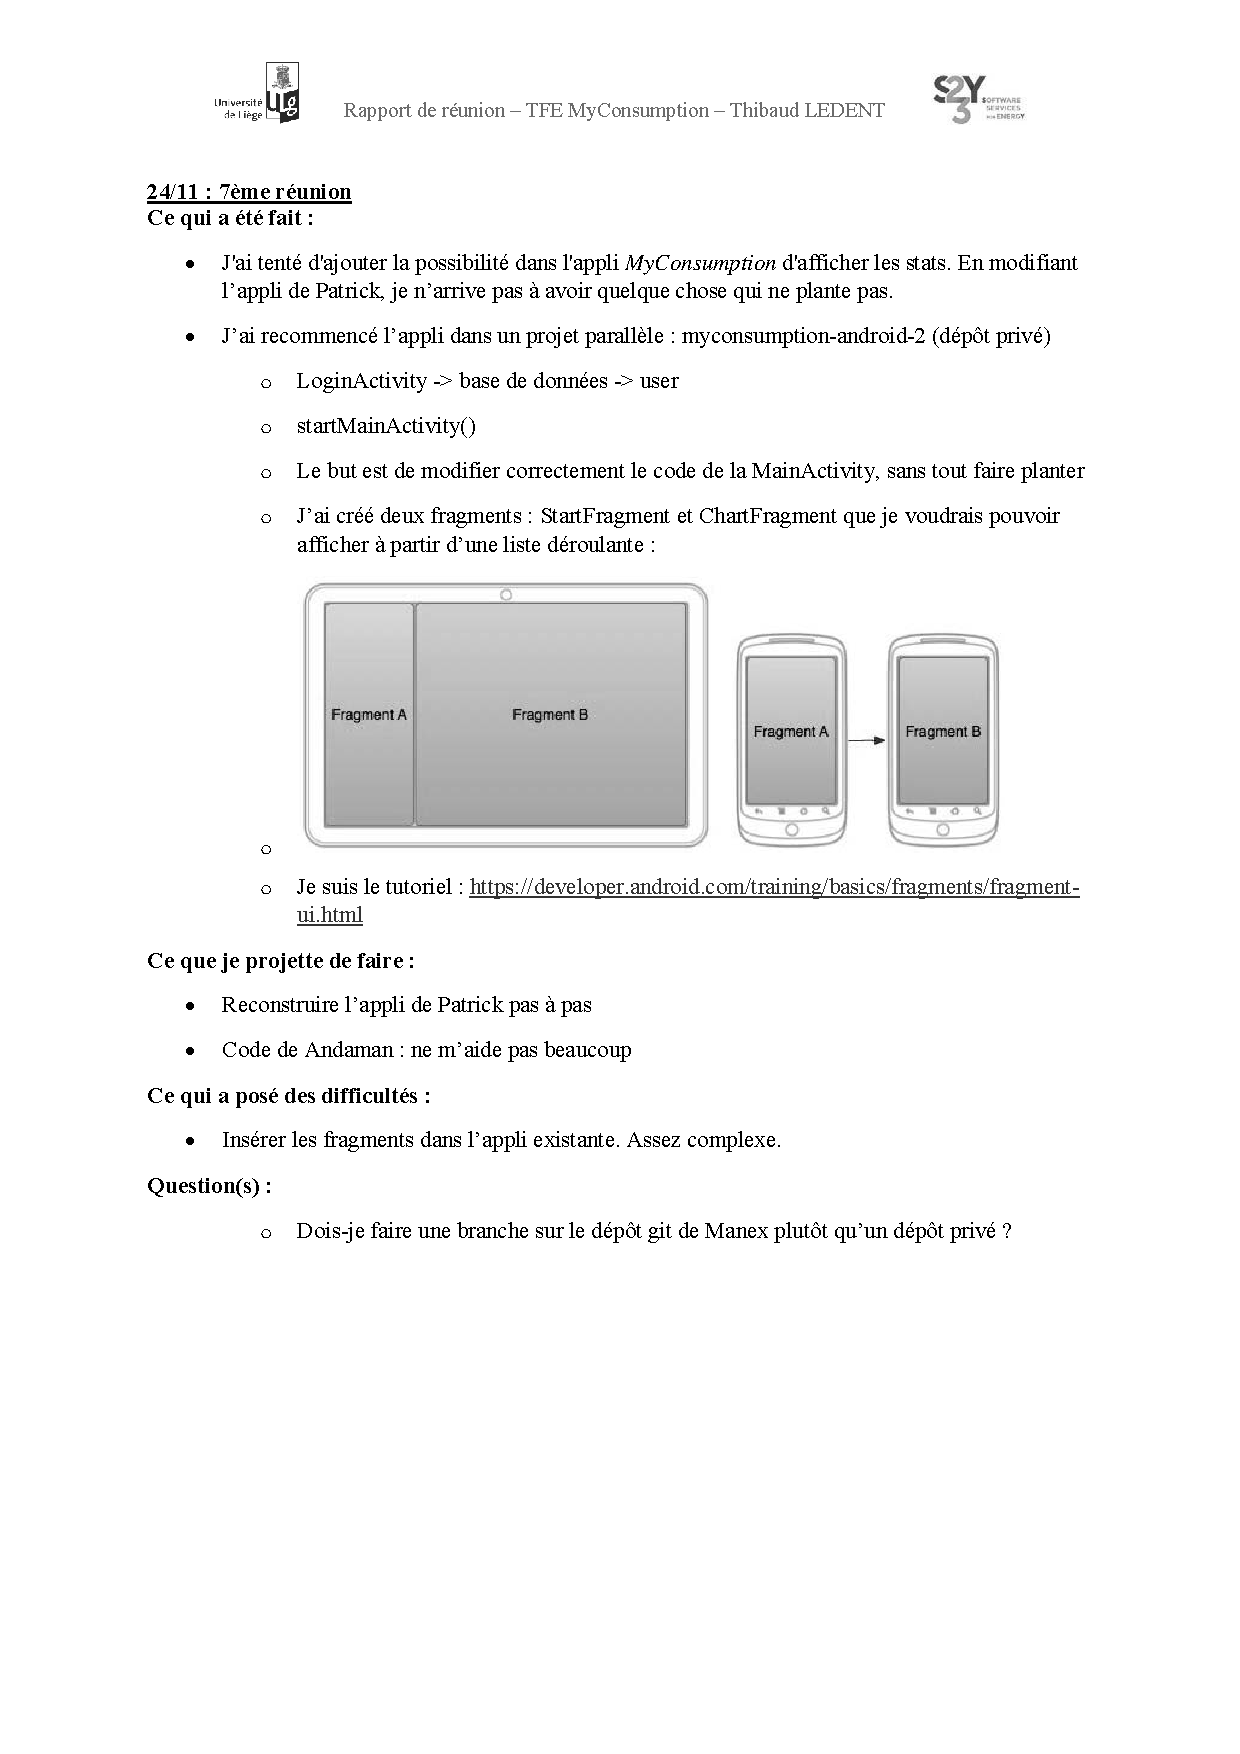
\includegraphics[width=1\textwidth]{reports_NB_Part7.pdf}
\newpage
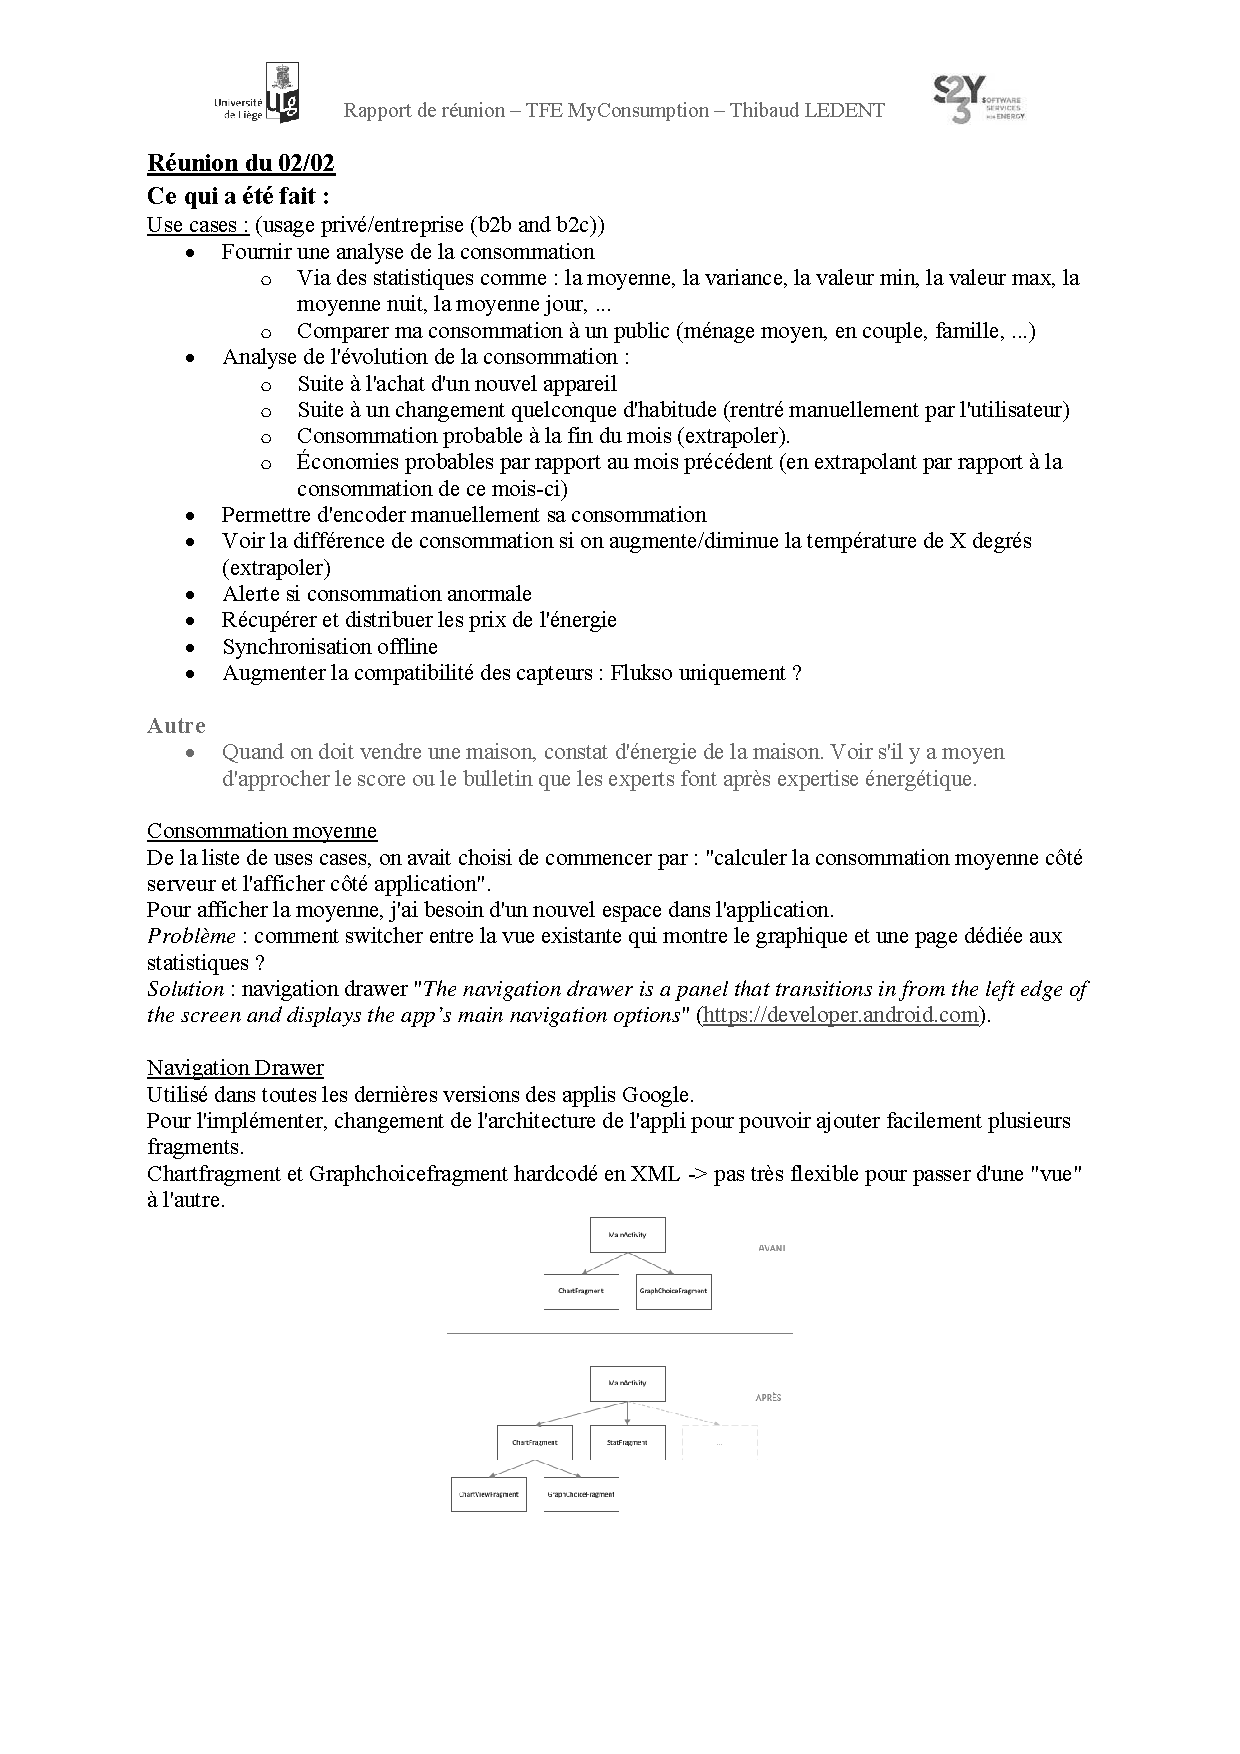
\includegraphics[width=1\textwidth]{reports_NB_Part8.pdf}
\newpage
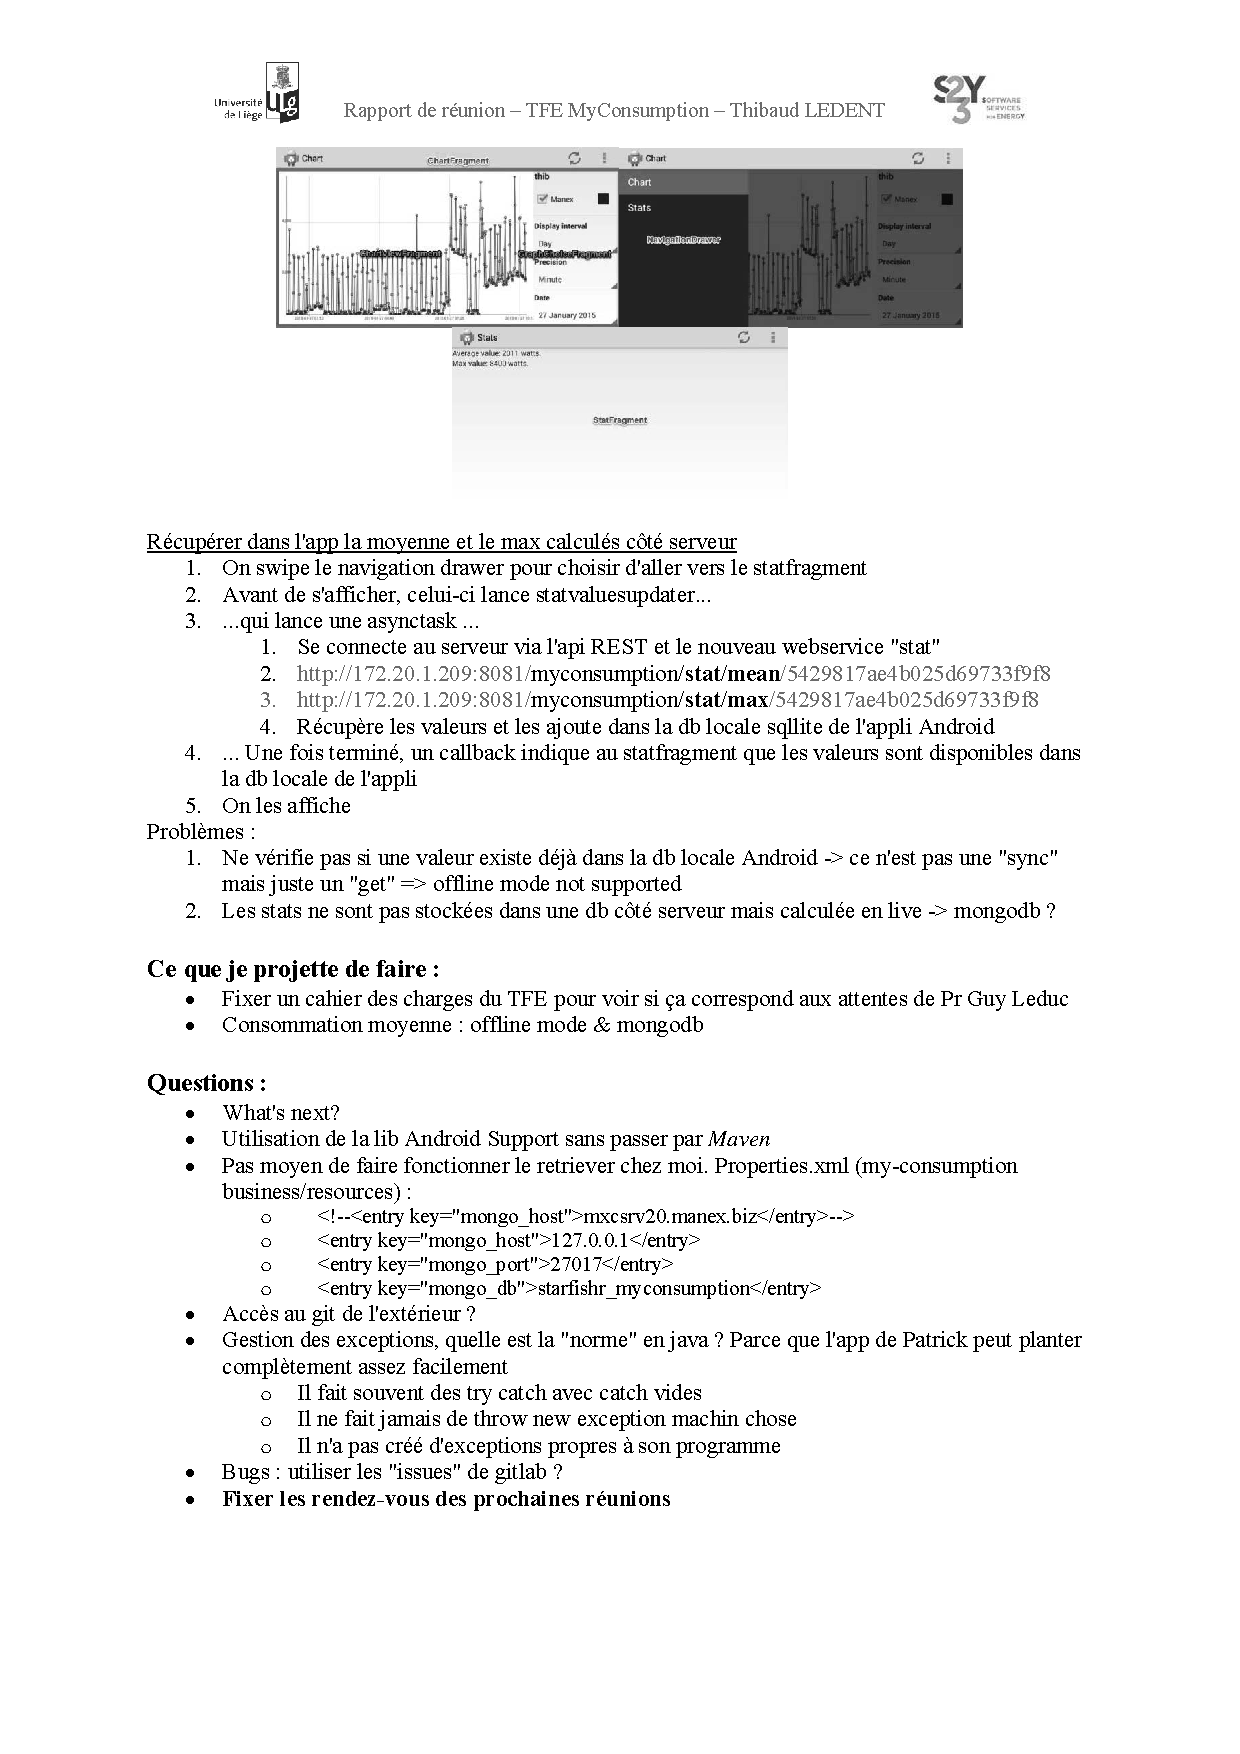
\includegraphics[width=1\textwidth]{reports_NB_Part9.pdf}
\newpage
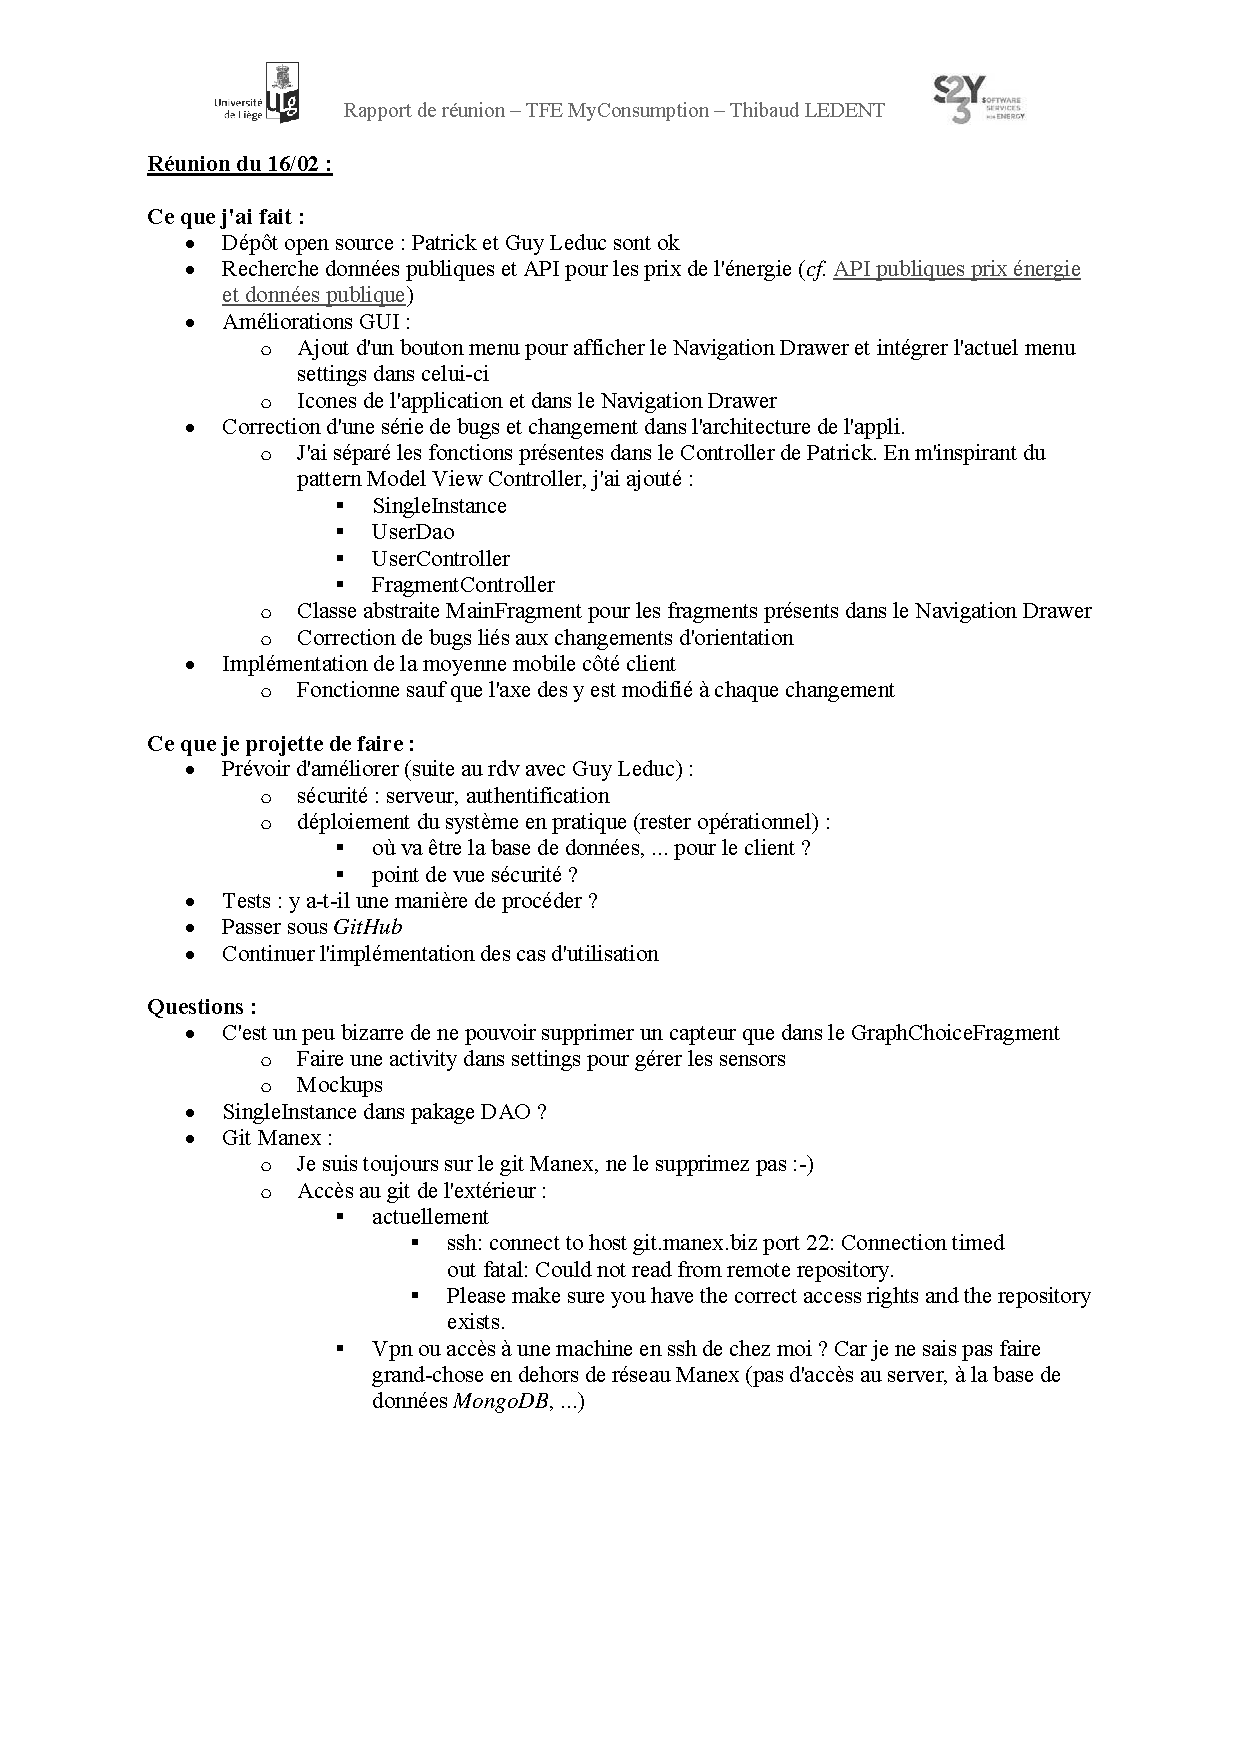
\includegraphics[width=1\textwidth]{reports_NB_Part10.pdf}
\newpage
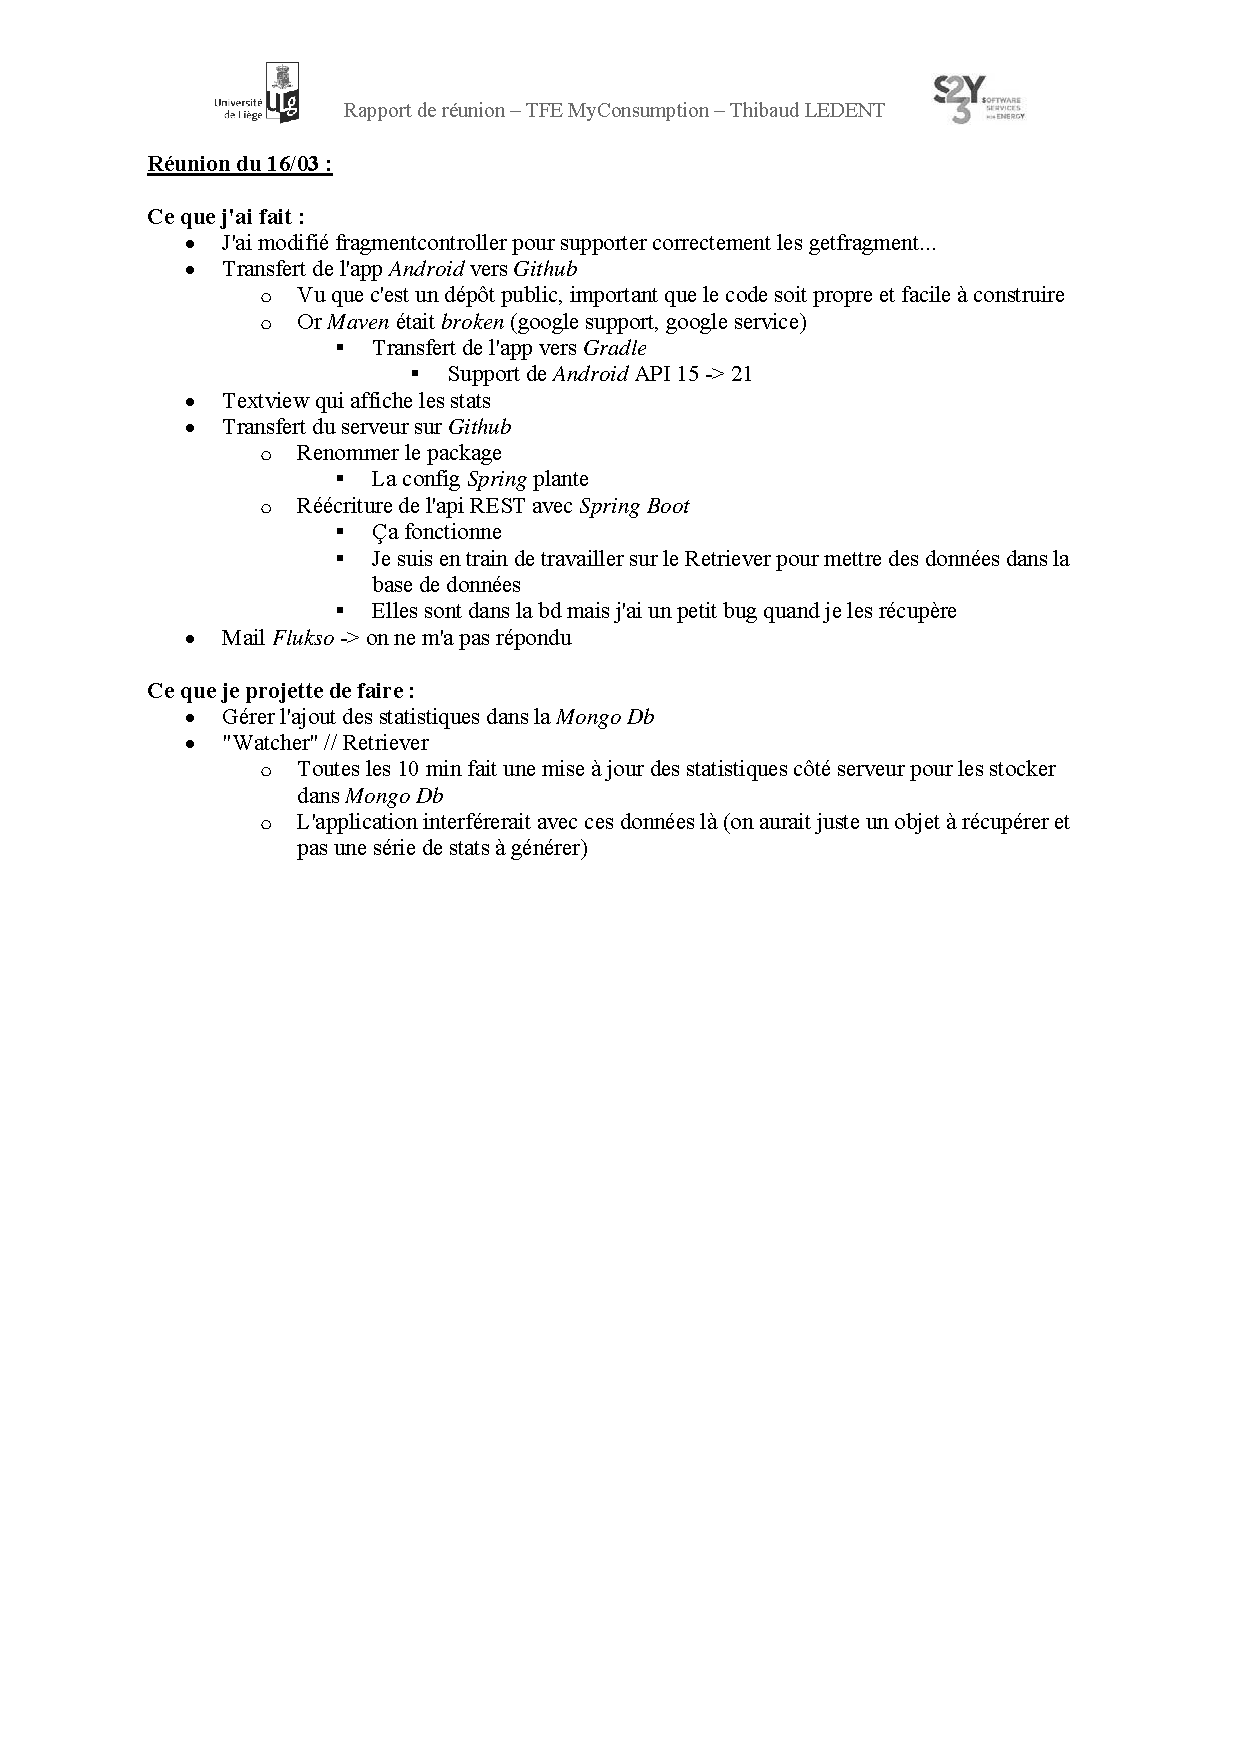
\includegraphics[width=1\textwidth]{reports_NB_Part11.pdf}
\newpage
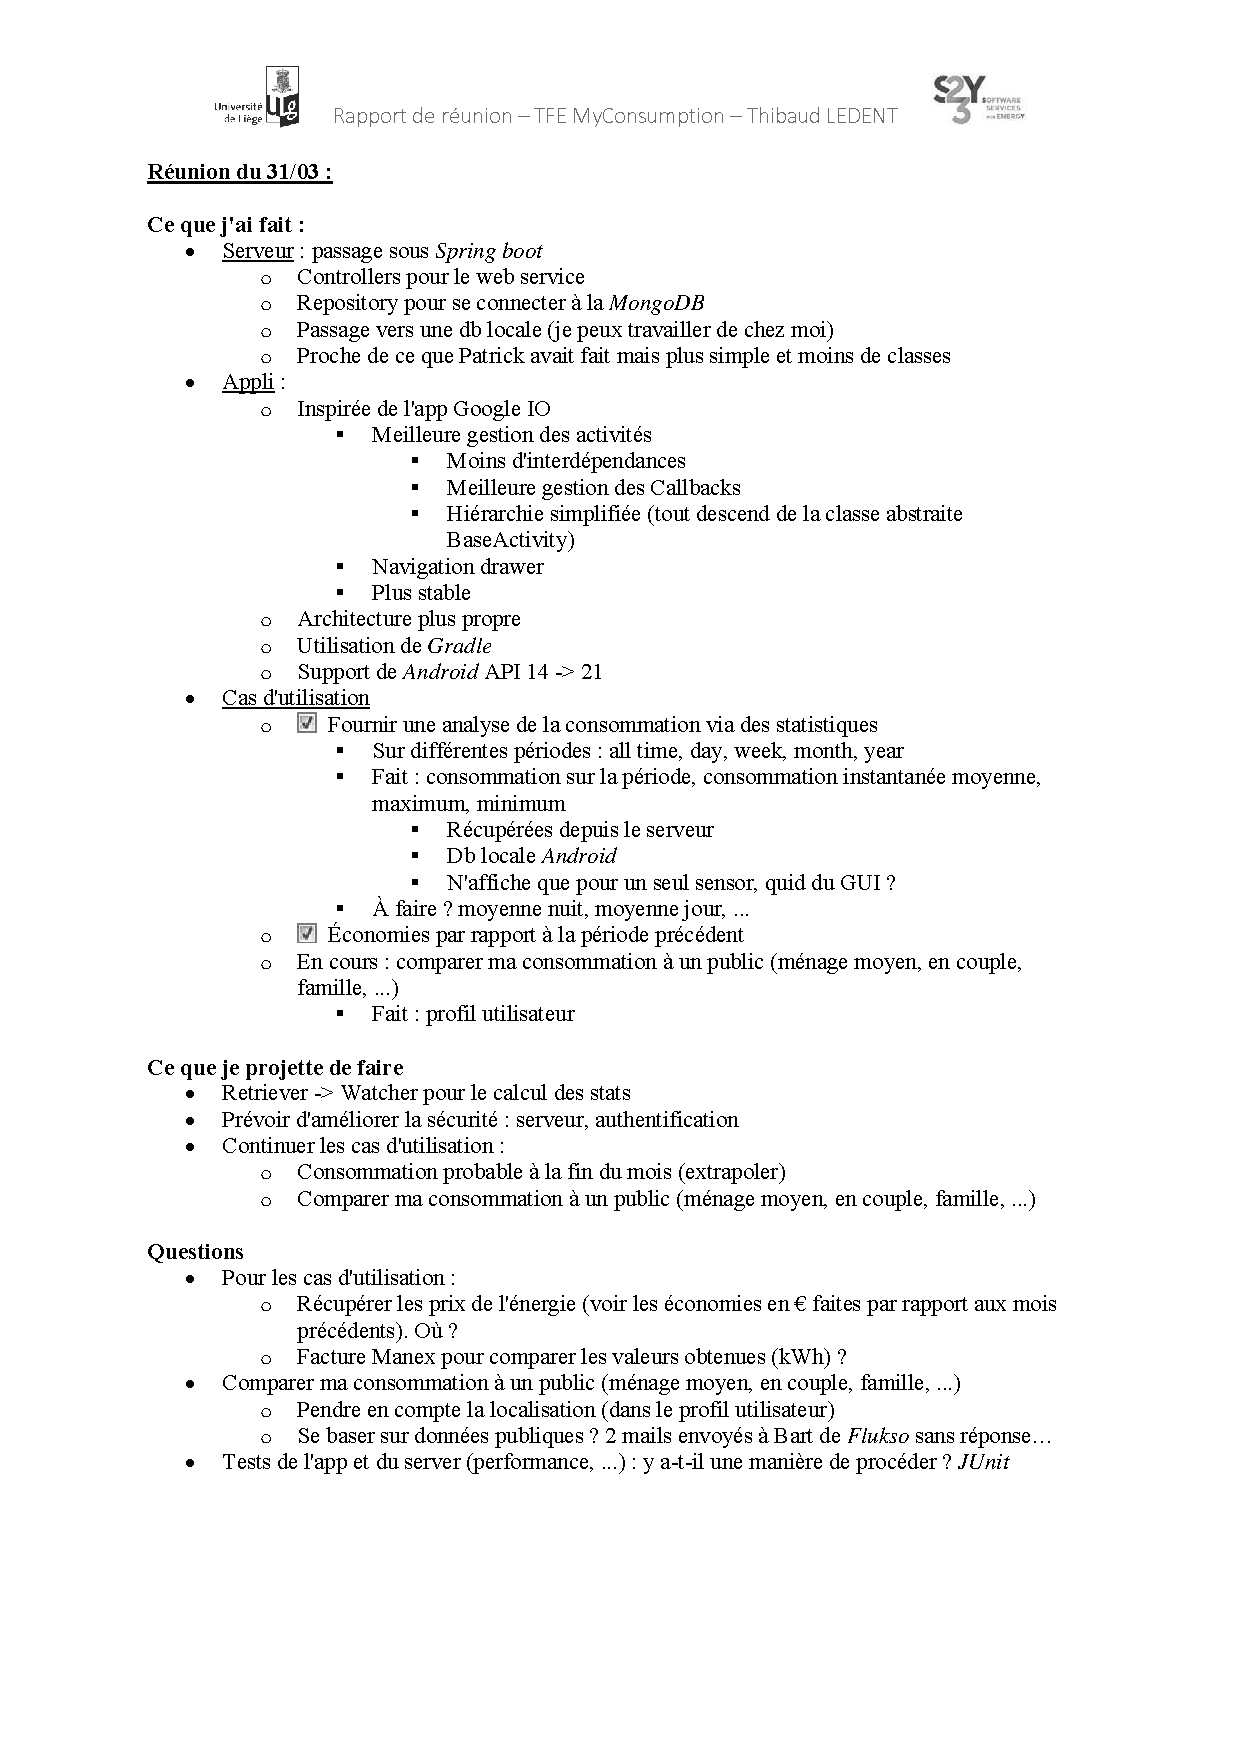
\includegraphics[width=1\textwidth]{reports_NB_Part12.pdf}
\newpage
\includegraphics[width=1\textwidth]{reports_NB_Part13.pdf}
\newpage
\includegraphics[width=1\textwidth]{reports_NB_Part14.pdf}
\newpage
\includegraphics[width=1\textwidth]{reports_NB_Part15.pdf}
\newpage
\includegraphics[width=1\textwidth]{reports_NB_Part16.pdf}
\newpage
\includegraphics[width=1\textwidth]{reports_NB_Part17.pdf}
\newpage
\includegraphics[width=1\textwidth]{reports_NB_Part18.pdf}

\backmatter

\part{Bibliography}
\renewcommand\partcontent{}


\bibliographystyle{myplain}
\bibliography{ref}


\end{document}